% Note that some parts of this document is generated from Javadoc comments using a special
% doclet called XMLConfigDoclet, which is included in the source code
% of ContactCenters.
% This doclet extends Texlet, which is used to produce LaTeX code from
% Java files containing LaTeX Javadoc comments.
% The build.xml file in the main directory of ContactCenters contains
% a mskdoc target which allows to compile this document automatically.

\documentclass[twoside, 12pt]{article}
\usepackage{tcode}
\usepackage{contactcenters}
\usepackage{xmlconfig}
\usepackage{ifpdf}
\usepackage[dvipsnames]{xcolor}
%\usepackage{crayola}
\usepackage[procnames]{listings}

\ifpdf
  \hypersetup{
     pdftitle={Generic Simulator for Blend and Multi-skill Call Centers},
     pdfauthor={Eric Buist},
     pdfsubject={User's Guide for ContactCenters Simulation Library},
     pdfkeywords={Contact centers, Simulation, SSJ, Java},
     pdfview=FitH,
     pdfstartview=FitH,
     pdfborder={0 0 0}
  }
\fi

\lstloadlanguages{Java,XML}
\lstset{language=Java,
floatplacement=htbp,
captionpos=t,
frame=trbl,
abovecaptionskip=1.5em,
belowskip=2em,
basicstyle=\small\ttfamily,
stringstyle=\color{OliveGreen},
commentstyle=\color{red},
identifierstyle=\color{Bittersweet},
basewidth={0.5em},
showstringspaces=false,
framerule=0.8pt,
procnamestyle=\bfseries\color{blue},
emphstyle=\bfseries\color{Cerulean},
procnamekeys={class,extends,interface,implements}
}

\usepackage{tikz}
\usetikzlibrary{arrows,shapes}

\setcounter{secnumdepth}{3}
\newcommand{\javadoc}[1]{}
\newcommand{\xmldoc}[1]{#1}
\newcommand{\javaxmldoc}[2]{#2}
\htmlexcludecomment{javadocenv}
\htmlincludecomment{xmldocenv}

%%%%%%%%%%%%%%%%%%%%%%%%%%%%%%%%%%%%%%%%%%%%%%%%%%%%%%%
\begin{document}
\begin{titlepage}
\null\vfill
\begin{center}
  {\Large\bf User's Guide for ContactCenters Simulation Library }\\[20pt]
  {\Large Generic Simulator for Blend and Multi-skill Call Centers} \\[20pt]
 Version: \today \\
\vfill
 {\sc Eric Buist}
\vfill
\end{center}

\vfill
This document introduces a generic
simulator for
blend and multi-skill
call centers.  The simulator is written
using Java, SSJ, and the ContactCenters library.
It is configured using
XML files and supports call centers with
inbound and outbound calls of multiple types,
multiple groups of agents, and complex routing policies.
This document presents the model implemented by the
simulator,
the format of the configuration files with some examples,
and instructions to
run the simulator from the command-line and to extend it internally in
Java code.
We also provide a reference guide documenting every supported
parameter and performance measure.
In this document, any reference to a contact corresponds to a call,
since the simulator only considers calls as type of contacts.
\end{titlepage}
\pagenumbering{roman}
\tableofcontents
\clearpage\listoftables
\clearpage\listoffigures
\clearpage\lstlistoflistings
\pagenumbering{arabic}

\part{Tutorial}
\section{Overview}

A \emph{contact center} is a set of resources (communication
equipment, employees, computers, etc.) providing an interface between
customers and a business \cite{ccMEH03a,ccGAN02a,ccAVR05b,ccAKS07a}.
Each \emph{contact} represents a customer reaching the contact center
to obtain some form of service.  The service is made by employees in
the contact centers called \emph{agents}.  Each agent is a member of
an \emph{agent group} which determines its characteristics
(skills, speed of service, etc.).
When a contact cannot be served immediately, it is put in a
\emph{waiting queue} to be served later.  The contact center
components are linked together by a \emph{router} which decides on how
to assign calls to agents.  A \emph{call center} is a
special form of contact center where each contact corresponds to a
telephone call.

The ContactCenters library is built using the Java
programming language \cite{iGOS00a}
and the Stochastic Simulation in Java (SSJ) library \cite{iLEC04j},
and permits one to implement
simulators for
contact centers.  The library provides building blocks such
as classes representing the contacts in the center, the agent groups,
the waiting queues, and the router.  The programmer combines these
blocks to make a simulator.
However, creating a simulator
directly using
this library involves Java programming.

This document presents a
ready-to-use generic simulator for the particular case of a blend and
multi-skill call center with multiple call types, agent groups and
simulation periods.  It can simulate \emph{inbound} calls arriving in
the system following a stochastic arrival process as well
as \emph{outbound} calls made by predictive dialers.  Service and
patience times are also random, and come from
any
probability distribution supported by SSJ, and parameters can change
from time periods to periods.

This simulator is configured
through XML files. Compilation of Java
code is not required, except if the simulator has to be extended,
or used internally by another program.
%  A XML file represents an hierarchical document composed of
%a root element which can have attributes as well as nested text and
%children elements.  Such a file can be
%created and modified with any text editor, but specialized editors
%dedicated to XML, e.g., XML Spy, are also available.
%  While XML specifies how to
%format elements and attributes in such a file,
%schemas indicate
%which structures are allowed for describing a specific concept.
Any XML document intended to be processed by a program conforms to a
schema.
The simulator uses one such schema for the
parameters of the simulated model, and a
second schema for the parameters of the experiment method.

% However, this simulator prevents the user from accessing all the
% possibilities of ContactCenters. If custom arrival processes, routing
% or dialing policies are needed, creating a full Java program using
% ContactCenters may be easier than trying to adapt the complex generic
% simulator.

The rest of this document is organized as follows.
In the next section, we present the call center model
implemented by the generic simulator.  We define the structure of
possible call centers as well as the supported types
of experiments.
Section~\ref{sec:mskconfig} introduces the format of the configuration
files for the simulator by some commented examples.  This is
a good way to learn how to make configuration files, not a
reference documentation.
Section~\ref{sec:mskuse} demonstrates how to run the
simulator from the command-line while section~\ref{sec:mskusejava}
shows how to interact with the simulator from a Java program.
Section~\ref{sec:msktrouble} discusses most common problems encountered
when using the simulator.
The last sections contain a reference manual
providing detailed documentation for each supported performance measure,
routing policies, dialing policies, arrival processes, the
supported types of experiments, and the format of generated reports.

Section~\ref{sec:mskxml}
gives a primer on XML, and the data types used in the
parameter files.
It also gives some examples on how parameter-specific documentation,
which is available in HTML only, can be retrieved.
The documentation for
each parameter was generated from the annotations in the
corresponding XML schemas, and can be located
in the \path{doc/schemas} subdirectory of ContactCenters.

\section{Simulation model}
\label{sec:mskmodel}

This section gives a description of the model implemented by the
simulator, without references to specific parameter names in the XML
configuration file.
See the next section for example configuration files,
section~\ref{sec:mskxml}
for a primer on XML and the data types used in parameter files,
and
the HTML documentation of the XML Schemas of ContactCenters for more
information on parameter names.

Figure~\ref{fig:ccmodel} gives an overview of the model implemented by
the simulator.  It shows that
calls are partitioned into $K$ \emph{call types} and
are sent to
agents partitioned into $I$ \emph{agent groups}.
Inbound calls arrive in the center from external sources while
outbound calls are produced by predictive dialers which are part of
the call center.
Calls that cannot be served immediately are queued, and abandon
if they cannot get service after a certain patience time.
However, the model is more complex than the figure shows:
the queueing discipline is not always first-in first-out,
routing can consider agents with multiple skills, and
parameters can change during the day.
The next sections will examine these aspects in more details.
%It can simulate multiple periods with different parameters in each
%one.  Inbound and outbound calls are supported as well as skill-based
%routing.

\begin{figure}
\centering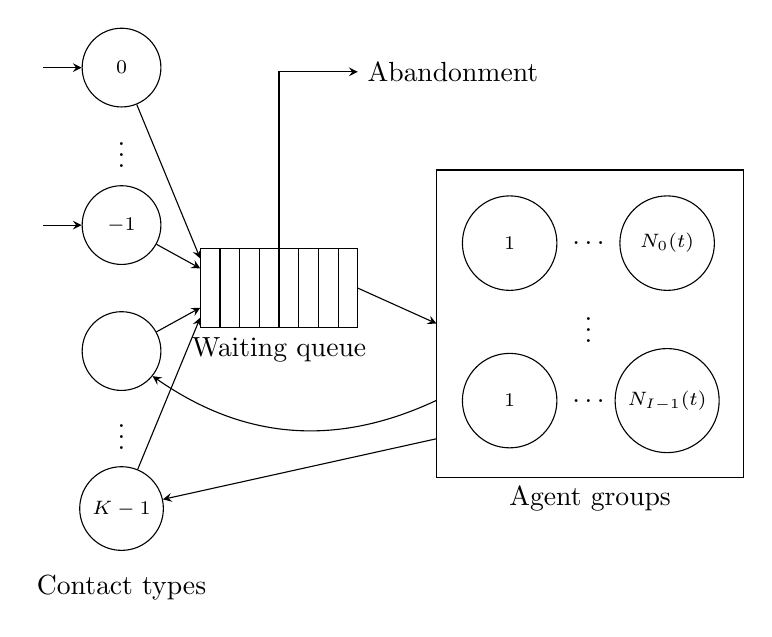
\begin{tikzpicture}[>=stealth]

\node (a1) [shape=circle,draw,minimum size=1.2cm] {{\scriptsize 1}};
\node (ai) [right of=a1] {$\ldots$};
\node (an) [right of=ai,circle,draw,minimum size=1.2cm] {{\scriptsize $N_0(t)$}};
\node (mid1) [below of=a1,shape=coordinate] {};
\node (mid) [below of=ai] {$\vdots$};
\node (midn) [below of=an,shape=coordinate] {};
\node (a21) [shape=circle,draw,below of=mid1,minimum size=1.2cm] {{\scriptsize 1}};
\node (a2i) [below of=mid] {$\ldots$};
\node (a2n) [below of=midn,circle,draw,minimum size=1.2cm] {{\scriptsize $N_{I-1}(t)$}};

\draw (a1.north west) +(-5mm,5mm) coordinate(topleftcorner)
(a2n.south east) +(5mm,-5mm) coordinate(bottomrightcorner);
\draw (topleftcorner) rectangle (bottomrightcorner);
\draw (topleftcorner |- bottomrightcorner) coordinate(bottomleftcorner);
\draw (topleftcorner -| bottomrightcorner) coordinate(toprightcorner);

\draw (topleftcorner) ++(-3,-2) coordinate(qbottomleftcorner)
rectangle ++(2,1) coordinate(qtoprightcorner);
\foreach \x in {0,0.25,...,2}
   \draw (qbottomleftcorner) ++(\x,0)
-- +(0,1);

\draw (qtoprightcorner |- qbottomleftcorner)
coordinate(qbottomrightcorner);
\draw (qtoprightcorner -| qbottomleftcorner)
coordinate(qtopleftcorner);

\path (bottomleftcorner)
 -- node [below] {Agent groups} (bottomrightcorner);
\path (qbottomleftcorner)
-- node [below] {Waiting queue} (qbottomrightcorner);

\draw (qtopleftcorner) ++(-1,2.3) node (k0) [shape=circle,draw,minimum size=1cm] {{\scriptsize $0$}};
%\node (kk) [below of=k0] {$\vdots$};
\draw (qtopleftcorner) ++(-1,0.3)
node (kK) [shape=circle,draw,minimum size=1cm]
{{\scriptsize $\Ki-1$}};
\path (k0) to
node (kk) {$\vdots$}
(kK);
\node (k0l) [left of=k0,shape=coordinate] {};
\draw[->] (k0l) -- (k0);
\node (kKl) [left of=kK,shape=coordinate] {};
\draw[->] (kKl) -- (kK);
\draw (qbottomleftcorner) ++(-1,-0.3)
node (ko0) [shape=circle,draw,minimum size=1cm] {{\scriptsize $\Ki$}};
\draw (qbottomleftcorner) ++(-1,-2.3)
node (koK) [shape=circle,draw,minimum size=1cm] {{\scriptsize $K - 1$}};
\path (ko0) to
node (kok) {$\vdots$}
(koK);
\node [below of=koK] {Contact types};

\path (qtopleftcorner) -- 
coordinate [very near start] (qcenterleft1)
coordinate [near start] (qcenterleft2)
coordinate [near end] (qcenterleft3)
coordinate [very near end] (qcenterleft4) (qbottomleftcorner);
\draw[->] (k0) -- (qcenterleft1);
\draw[->] (kK) -- (qcenterleft2);
\draw[->] (ko0) -- (qcenterleft3);
\draw[->] (koK) -- (qcenterleft4);
\path (topleftcorner) --
coordinate [near end] (centerleft1)
coordinate [very near end] (centerleft2)
(bottomleftcorner);
\draw[->] (centerleft1) to [bend left] (ko0);
\draw[->] (centerleft2) -- (koK);

\path (qtoprightcorner) -- 
coordinate (qcenterright)
(qbottomrightcorner);
\path (topleftcorner) --
coordinate (centerleft)
(bottomleftcorner);
\draw [->] (qcenterright) -- (centerleft);

\draw (topleftcorner) ++(-1,1) node (ab) [above right] {Abandonment};
\path (qtopleftcorner)
--
coordinate(qtopcenter)
(qtoprightcorner);
\draw[->] (qtopcenter) |- (ab);
\end{tikzpicture}


\caption{The Implemented Model of Call Center}
\label{fig:ccmodel}
\end{figure}

\subsection{The simulation horizon divided into periods}
\label{sec:periods}

The simulation horizon can correspond to a day, a week, a month, etc.
As shown on figure~\ref{fig:periods},
it is divided into $P+2$ time
intervals called \emph{periods}.
The call center's opening hours are divided into $P$ \emph{main periods}
with fixed duration $d$.
For example, these periods may correspond to
half hours or hours in
the simulated horizon.
Main period~$p=1,\ldots,P$ corresponds to the
time interval $[t_{p-1}, t_p)$, where $0 \le t_0 < \cdots < t_P$.
During the \emph{preliminary period} $[0, t_0)$, no agent is available
to serve calls but arrivals can start a few minutes before $t_0$ for a
queue to build up.
During the \emph{wrap-up period} $[t_P, T]$, where $T$ is the time at
which the simulation ends and the center is completely empty, no
arrival occurs, but in-progress services are terminated.

\begin{figure}
\centering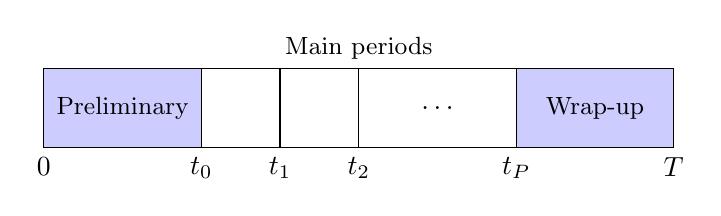
\begin{tikzpicture}[>=stealth]
\draw [fill=blue!20] (0,0) rectangle (2,1);
\draw [fill=blue!20] (6,0) rectangle (8,1);
\draw (0,0) rectangle (8,1);
\foreach \x/\xtext in {0, 2/$t_0$, 3/$t_1$, 4/$t_2$, 6/$t_P$, 8/$T$}
    \draw (\x,1) -- ++(0,-1) node [below] {\xtext};
\node at (1,0.5) {{\small Preliminary}};
\node at (5,0.5) {$\ldots$};
\node at (7,0.5) {{\small Wrap-up}};
\node at (4, 1) [above] {{\small Main periods}};
\end{tikzpicture}


\caption{The simulated horizon}
\label{fig:periods}
\end{figure}

Parameters are usually specified for the main periods only.  During
the preliminary
period, there are no agents to serve calls and if other parameters are
needed, the simulator takes them from the first main
period.  During the wrap-up period, the parameters from the last main
period are used.
The preliminary and wrap-up periods can have a length of 0
in several models.  They are useful to simulate one day starting where
$t_0>0$.  Since the preliminary and wrap-up periods are secondary,
main periods are often denoted as
the periods in the rest of this document.

\subsection{The processing of a call}

The set of $K$ call types is divided into two subsets:
$\Ki\le K$ inbound call types with indices $0, \ldots, \Ki - 1$,
and $\Ko$ outbound call types with indices $\Ki, \ldots, K - 1$.
Each call type can have its own \emph{call source} which produces
only calls of this type, and can be
shut up and down at any time during the simulation.
In addition, call sources producing calls of multiple, randomly-chosen
types, can be defined.
In the latter case, if a call is generated during main period~$p$,
its type is $k$ with a fixed probability
$p_{k,p}$,
independently of other calls.
The way calls are produced depends on whether they are inbound or
outbound, and will be covered in the next subsections.
% The \emph{service time}, i.e., the time spent by a call with an agent,
% can depend on the period~$p$ of arrival,
% the call type~$k$ as
% well as the agent group~$i$ assigned by the router.
% Let $1/\mu_{k, p}$ be the call type-dependent mean service time and
% $1/\mu_{k,
%   i, p}$ be the mean service time depending on call type and agent group.

% A call of type~$k$ entering the system during period~$p$ that cannot
% be served
% immediately balks, i.e., abandons
% without being served or waiting in queue, with probability $\pi_{k,
%   p}$.  If it does not balk,
% before abandoning or being served, it waits for a maximal
% \emph{patience time} with mean $1/\nu_{k,p}$, which can have any
% period-specific probability distribution.

Figure~\ref{fig:callpath} shows the path of a call into
the call center.
On this figure, rectangles represent processing steps for
the call while diamonds represent conditional branching.
The rectangle with thick lines represents the starting point of the
calls in the system.
An ellipse denotes an outcome for a call (blocking, service,
or abandonment).
When a call arrives, a free agent is selected among the $I$ agent groups.
The router (see section~\ref{sec:routergeninfo}) uses
the type of the call to determine
which agents are allowed to serve the call,
and how agents are chosen if several agents are free.
If a free agent is found, the call is sent to that agent, and
the agent is allocated for a certain \emph{service time}.
Conditionally on the call type, agent group and period of arrival of
the call, service times are i.i.d.\ and follow any parametric
probability distribution supported by SSJ.
If no agent is available for a new call, the call is sent to a waiting
queue if that does not exceed the total queue capacity.
With some probability depending on the call type
and the arrival period, independently of other events, the caller
entering queue
\emph{balks}, i.e., it abandons
immediately.  Other calls
having to wait go into a queue where they remain
until agents are free to serve them.
A queued caller can also become impatient, and abandon without
service.
Patience times are i.i.d.\ conditional to call type, and arrival period.
If the queue is full at the time of a call's arrival,
the call is \emph{blocked} instead of entering the queue, i.e., the
caller
receives a busy signal.

\begin{figure}
\centering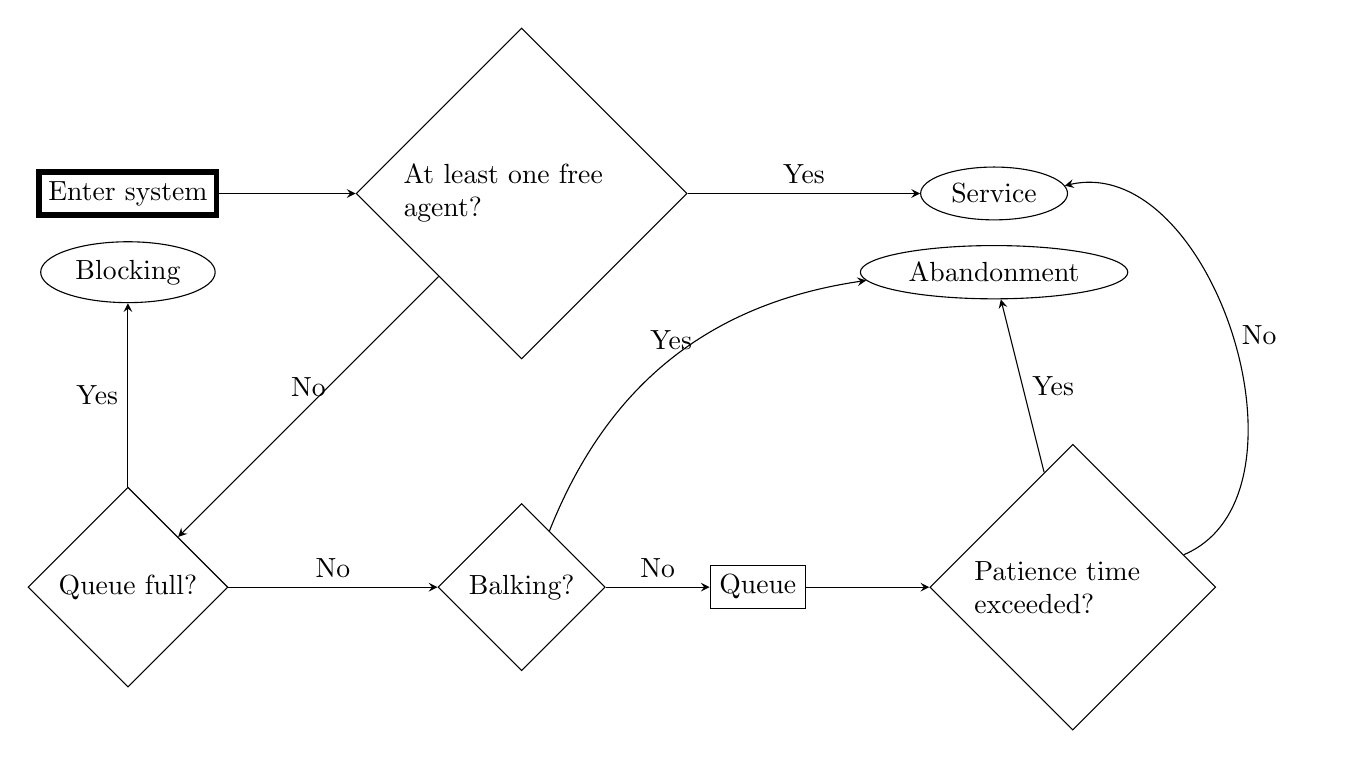
\begin{tikzpicture}[shape=rectangle,>=stealth]
\node (ap) [draw,line width=2pt] {Enter system};
\node (ifq) [draw,shape=diamond, node distance=5cm, below of=ap] {Queue full?};
\node (ifa) [draw,shape=diamond, node distance=5cm, right of=ap, text width=3cm] {At
  least one free agent?};
\node (balk) [draw,shape=diamond, node distance=5cm, right of=ifq]
{Balking?};
\node (q) [draw, right of=balk, node distance=3cm] {Queue};
\node (ifp) [draw,shape=diamond, node distance=4cm, right of=q, text width=2.5cm]
{Patience time exceeded?};

\node (bl) [draw, shape=ellipse, below of=ap] {Blocking};
\node (sr) [draw, right of=ifa, node distance=6cm, shape=ellipse] {Service};
\node (ab) [draw, below of=sr, shape=ellipse] {Abandonment};

\draw[->] (ap) -- (ifa);
\draw[->] (ifq) edge 
node [left] {Yes}
(bl)
edge 
node [above] {No}
(balk);
\draw[->] (ifa) edge
node [above] {Yes}
(sr)
edge
node [above] {No}
(ifq);
\draw[->] (balk)
edge [bend left]
node [above] {Yes}
(ab)
edge
node [above] {No}
(q);
\draw[->] (q) -- (ifp);
\draw[->,bend angle=85] (ifp)
edge
node [right] {Yes}
(ab)
edge [bend right]
node [right] {No}
(sr);
\end{tikzpicture}


\caption{The path of a call in the call center}
\label{fig:callpath}
\end{figure}

An agent finishing a service can disconnect for a random duration
before it takes new calls.
The probability and duration
of disconnecting may depend on the agent group, and
the time period.
By default, the probability is 0, so no disconnecting occurs.

\subsubsection{Inbound calls}

\emph{Inbound calls} are produced using
some \emph{arrival processes}.  Such a process generates
random inter-arrival times following some possibly
non-stationary distributions, and generates a single call upon each
arrival.  The most common distribution for inter-arrival times is
exponential, which results in a Poisson arrival process.
The simulator supports some variants of the Poisson process with
time-varying or stochastic arrival rates.
See
section~\ref{javadoc:umontreal.iro.lecuyer.contactcenters.app.ArrivalProcessType}
for more details.

\subsubsection{Outbound calls}

\emph{Outbound calls} are produced
using a predictive \emph{dialer}
which makes outbound calls when
certain conditions apply.  There can be one dialer for each outbound call
type as well as dialers producing outbound calls of multiple,
randomly-chosen, types.

When a dialer is started, it tries to perform outbound calls
each time an agent capable of serving calls produced by the
dialer becomes free.
Each time the dialer is triggered, it decides on how many calls to
try, and processes each of these calls independently,
as shown on
figure~\ref{fig:outbound}.
First, dialing succeeds with a reaching
probability depending on the call type and period.
A delay depending on the success of the call, the call type, and the
period of dialing then occurs.
The dialing delay can be used to model the party's phone ringing while
a failed call may represent a busy signal, answering machine, etc.
Successful calls are processed in a similar
way as inbound calls while failed calls simply leave the system after
they are counted.
During the processing of a successful call, the period of arrival
corresponds to the period during which the dialer decided to make a
call, not the period during which the call entered the call center.

The only difference when processing inbound calls and successful
outbound calls is
the service time which includes a \emph{preview time} that
can be used to model the work made by the agent to determine
if the right party is reached.
The same way as service times,
preview times are i.i.d.\ but can depend on the call type, agent
group,
and period of arrival.
After this preview time,
with some probability depending on the call type and period of
arrival, the call is a right party connect, and enters regular service.
The preview and regular service times are generated
independently, and summed up in the case of right party connects. In other words,
the time the agent spends with an outbound
call is the sum of the preview and service times.
On the other hand,
if the call is a wrong party connect, it is counted separately and
excluded from reports concerning served calls.
The service of a wrong party connect only consists of a preview time.

No further special processing is applied to outbound calls
in this model.  However, some parameters can
be adapted to outbound calls.
For example, a called customer often balks (or
abandons very quickly) if no agent is available to serve him.
In fact, any outbound call that needs to wait is called a
\emph{mismatch}, and
is avoided in most call centers.
Consequently, the average patience time of any outbound call should be
small.

\begin{figure}
\centering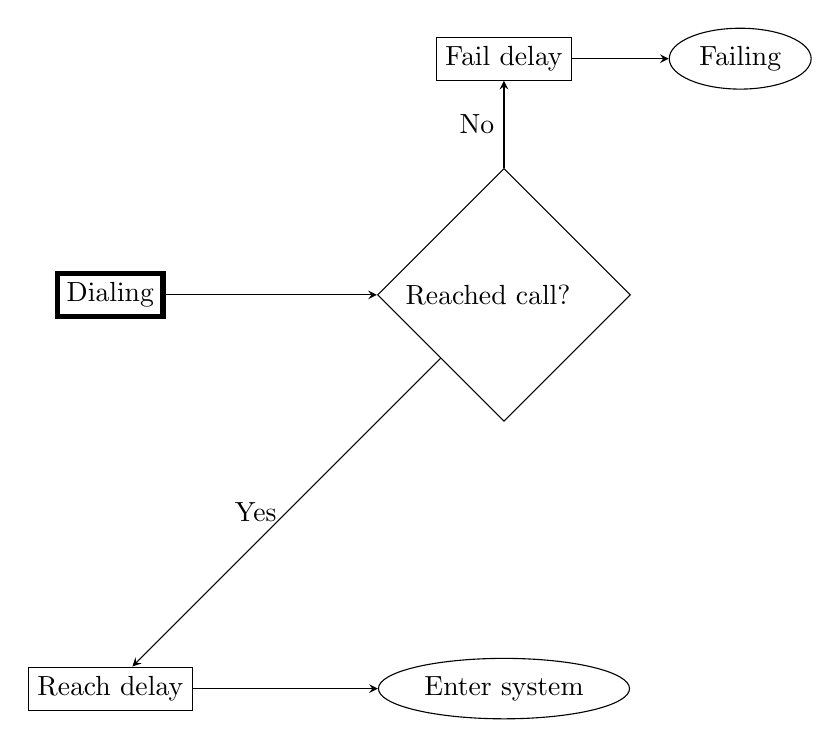
\begin{tikzpicture}[shape=rectangle,>=stealth]
\node (dialing) [draw, line width=2pt] {Dialing};
\node (rpc) [draw, shape=diamond, node distance=5cm, right of=dialing,
text width=2.5cm]
{Reached call?};
\node (failtime) [draw, node distance=3cm, above of=rpc]
{Fail delay};
\node (fail) [draw, shape=ellipse, right of=failtime, node distance=3cm]
{Failing};
\node (reachtime) [draw, node distance=5cm, below of=dialing]
{Reach delay};
\node (ib) [draw, shape=ellipse, node distance=5cm, right
of=reachtime]
{Enter system};


\draw[->] (dialing) -- (rpc);
\draw[->] (rpc)
edge
node [left] {Yes}
(reachtime)
edge
node [left] {No}
(failtime);
\draw[->] (failtime) -- (fail);
\draw[->] (reachtime) -- (ib);
\end{tikzpicture}


\caption{The path of an outbound call in the call center}
\label{fig:outbound}
\end{figure}

The dialer uses a \emph{dialer's policy} to determine how many calls
to dial each time it is triggered.
%For this, the policy often uses the number of agents in a \emph{test
%  set} of groups that contains all agent groups in the call center.
%The set of agent groups from which the dialer gets the number of free
%agents capable of serving the dialed calls is named the \emph{target
%  set}, and the target set for dialer~$k$ is composed of all agents
%capable of serving calls of any type produced by that dialer.
Let $\Ntf(t)$ be the total number of free agents, or
equivalently the number of free agents in the \emph{test set}, at simulation
time~$t$.  Also let
$\Ndf[k](t)$ be the total number of free agents capable of serving
some calls produced by dialer~$k$, or equivalently the number of free agents in the
\emph{target set} for dialer~$k$, at simulation time~$t$.

A common dialing condition checks that $\Ntf(t)\ge s_{\mathrm{t}, k}(t)$,
and $\Ndf[k](t)\ge s_{\mathrm{d}, k}(t)$, where
$s_{\mathrm{t}, k}(t)$ and
$s_{\mathrm{d}, k}(t)$ are user-defined thresholds. Their values are
constant during periods but can change from periods to periods.
The number of calls to dial at a time is computed from $\Ndf[k](t)$ in
a way depending on the selected \emph{dialing policy}.
See
section~\ref{javadoc:umontreal.iro.lecuyer.contactcenters.app.DialerPolicyType}
for more information.

% When an outbound call of type~$k$ is made during period~$p$,
% a \emph{right party connect} occurs with
% probability
% $\rho_{k, p}$.  When a right party connect occurs, the resulting successful call
% reaches the router for further processing.
% Otherwise, the call is
% a failed call which is counted for statistical collecting only before it
% disappears.  Some period-specific
% random delay, which is set to~0 by default,
% is needed for the dialer to determine if a call
% succeeds or fails.

\begin{comment}
\subsection{The attributes of a call}
\label{sec:callattr}

At the time of its creation, a call gets some attributes: a type index
$k$, a
patience time, and $I$ service times.
All these attributes are random variates generated at the time the
call arrives.
The call type determines the distribution of these
random variables as well as a period-specific probability of balking,
When balking occurs, the patience time is 0 independently of the
specified distribution.
The patience time is used for abandonment while the
service time $i$ is used if the call is served by an agent in group~$i$.
The $I$ service times are equal if service times do not depend on the
selected agent.

Acceptable waiting times $s_{k, \pawt}$, $\sK{k}$,
$\sP{\pawt}$, and $s$ are thresholds
used for estimating quantities such as the service level
in the case of inbound calls.
These thresholds, which are often equal, depend only on the call type,
and the AWT period $\pawt$ of the call, the latter period
index depending on how the simulation is performed.
For a simulation on a finite horizon  (see section~\ref{sec:simoutput}),
$\pawt$ corresponds to the statistical period $\pstat$ of the call,
which usually corresponds to its period of arrival.
For a steady-state simulation,
$\pawt$ corresponds to the period simulated at steady state.
%The threshold used depends on the call type and
%time interval for which the
%performance measure is estimated.
For example, the number of calls of type~$k$ during the whole horizon
served before the threshold is determined using $\sK{k}$ while the
number of calls of type~$k$ and statistical period $\pstat$
is determined using $s_{k, \pawt}$.

Outbound calls have additional attributes: the
result of a test determining if it succeeds (i.e., right party
connect) or fails, and
the random delays between the time the dialing and
the success or failure of the call.
The outbound call type determines the probability of right party
connect for each main period as well as the distribution for reach and
fail times.

After it exits the system, a call gets some additional attributes: a
waiting time (which can be 0 if the call was served immediately), and
a statistical period $\pstat$.  This second period index
also depends on how the simulation is performed, but it usually
also corresponds to the period of arrival of the call.
Table~\ref{tab:callperiods} gives the default value of the AWT and
statistical periods for both supported experiment types.

\begin{table}
\caption{The periods of a call}
\label{tab:callperiods}

\centering
\begin{tabular}{|l|l|l|} \hline
Horizon & $\pawt$ & $\pstat$ \\ \hline
Finite (see section~\ref{sec:expfinite}) & $\pstat$
& Period of arrival \\
Infinite (see section~\ref{sec:expsteadystate}) & $p$ & 0 \\
\hline
\end{tabular}
\end{table}
\end{comment}

\subsection{The agent groups}

Each agent group~$i$ has a fixed number $N_i(t)$  of agents
at any time during the simulated horizon.
%This number can
%change from periods to periods, but is often constant inside
%a period.
In this model, the function $N_i(t)$ is piecewise-constant.
If $N_i(t)$ increases at a given time $t$, the additional
agents are notified to the router which assigns them queued calls, if
possible.
The type of the queued call assigned to a new agent in group~$i$
depends on the routing policy being used.

Often, agents are added in several groups at a given time $t$,
corresponding, e.g., to the beginning of a main period.
In such a case, the router notifies all new agents in group~0 to the
router before notifying agents in groups~1, 2, etc.
The order in which the agents are notified to the router may have a
small impact on which queued calls are assigned to which agent groups,
but this only affects a few calls.

If $N_i(t)$ decreases at a given time $t$, no particular event
happens, except if $N_i(t)$ becomes smaller than
$\Nb[i](t)$.
The behavior of the system when that occurs
depends on how the agent group is modeled, but an agent
always terminates its on-going service before it can leave.

Only a fraction of the available agents is allowed to
serve calls.  If there is no busy agent, the total number of
agents free to serve calls is given by $\epsilon_i N_i(t)$ rounded to
the nearest integer, where $\epsilon_i\in[0, 1]$ is the
\emph{efficiency} of the agent group.  If $\epsilon_i=1$, all agents
are allowed to serve calls.

Agent groups can be modeled two ways by the simulator: with counters
representing the number of agents in each state, or with entities
representing each individual agent.
With the first model, the agent group only retains the number of
agents which are busy, free, and idle but unavailable to serve calls.
When $N_i(t)<\Nb[i](t)$, on-going services
are finished, and the group does not accept any call until
$\Nb[i](t) < N_i(t)$.
However, in the second model, the so-called \emph{detailed} group is
composed of
separate agents with their own states.
In that case, when $N_i(t)<\Nb[i](t)$,
some agents are marked to leave the system, but other busy agents
might finish their services before these marked agents leave.
As a
result, a detailed group can accept new calls even when
$\Nb[i](t)>N_i(t)$.
Which agents are marked is not relevant, because all busy agents are
identical in the model.
Detailed agent groups are more realistic, and allow for computing the
longest idle time of agents, which is needed by some routing
policies. However, using counter-based agent groups can increase
performance compared to detailed groups.

The $N_i(t)$ functions can be specified three ways: with a staffing
vector, with a schedule, or with individual agents.
In the first setting, $N_i(t)$ remains constant during individual
periods.
When specifying a schedule, one gives a set of shifts with arbitrary
starting and ending times, and assigns some agents to each shift.
With the third mode, one assigns each individual agent
any user-defined properties in addition to a shift.

\subsection{The router}
\label{sec:routergeninfo}

A \emph{router} assigns agents to inbound calls and successful
outbound calls (\emph{agent selection} or
\emph{push routing}), and
queued calls to free agents (\emph{call selection} or
\emph{pull routing}), using
a \emph{routing policy} to take its decisions.
The model supports a set of predefined routing policies (see
section~\ref{javadoc:umontreal.iro.lecuyer.contactcenters.app.RouterPolicyType})
that can be parametrized by the user.

The waiting queue
represented on figure~\ref{fig:ccmodel}
is partitioned into several
elementary waiting queues implemented as lists.
The number of waiting queues,
and the way they are used
depends on the routing policy.  Most routing policies assign a
waiting queue to each contact type, and all policies supported by the
simulator use a First In First Out (FIFO) discipline in individual
queues.

Parameters for the routing policy are encoded in one of the three main data
structures: a set of ordered lists,
incidence matrices, or matrices of ranks.  When the first
structure is used, the
\emph{type-to-group map} defines an ordered list of agent groups
$i_{k, 0}, i_{k, 1}, \ldots$ for each call type~$k$.  These lists give the order
in which agent groups are tested during agent selection.
The \emph{group-to-type map} defines an ordered list
of call types $k_{i, 0}, k_{i, 1}, \ldots$ for each agent group~$i$.  These lists
are used during call selection to determine the order in which
call types are tested.
These routing tables are represented by non-rectangular 2D arrays of integers.
In the type-to-group map, there is one row for each call type whereas
in the group-to-type map, there is one row per agent group.
Any negative integer
in these 2D arrays being ignored, they can be used for padding.
For an example of a routing policy using this structure, see
\texttt{QUEUEPRIORITY} in
section~\ref{javadoc:umontreal.iro.lecuyer.contactcenters.app.RouterPolicyType}.

The second possible structure is a pair of incidence matrices.
The \emph{type-to-group incidence matrix}
defines a
boolean function $\iTG(k, i)$ which determines if
calls of type~$k$ can be routed to agents in group~$i$.
The \emph{group-to-type incidence matrix}
defines a similar function
$\iGT(i, k)$ that determines if a call of type~$k$ can be selected
by a free agent in group~$i$.
Often, $\iTG(k, i)=\iGT(i, k)$, i.e., a call of type~$k$ can be sent
to an agent in group~$i$ if and only if a free agent in group~$i$
can select a call of type~$k$.
These matrices are encoded into 2D arrays of booleans.
This structure is not used by any router at this moment.

When the third structure is used,
the \emph{matrices of ranks}, which can also be named the priority matrices,
define functions
$\rTG(k, i)$ and
$\rGT(i, k)$ giving the rank, i.e., priority,
of agents in group~$i$ for calls of type~$k$.  The lower the rank, the
higher is the preference of the call type~$k$ for the agents in
group~$i$.  When a rank is
$\infty$, calls of type~$k$ cannot be served
by agents in group~$i$.
The matrix defining the
type-to-group ranks
$\rTG(k, i)$,
specifies how
contacts prefer agents, and is used for agent selection.
On the other hand,
the second matrix
defining the group-to-type ranks
$\rGT(i, k)$ specifies how agents prefer
contacts, and is used for contact selection.
In many cases, it is possible to have $\rGT(i, k)=\rTG(k, i)$ and
specify a single matrix of ranks.
These functions are encoded into rectangular 2D arrays of integers
containing, in the case of agent selection,
one row for  each contact type and one
column for each agent group.  For contact selection matrices of ranks,
the roles of rows and columns are inverted.
Although this structure is more flexible than ordered lists, it is
often less intuitive
to figure out the implied routing.
For an example of a routing policy using this structure, see
\texttt{AGENTSPREF} in
section~\ref{javadoc:umontreal.iro.lecuyer.contactcenters.app.RouterPolicyType}.

% A third structure, \emph{incidence matrices}, is available but
% currently unused by routing policies. The type-to-group incidence
% matrix is similar to the type-to-group matrix of ranks, except that
% $\rTG(k, i)$ is a boolean indicating if the router allows calls of
% type~$k$ to be served by agents in group~$i$.
% A similar group-to-type incidence matrix can also be defined.

\begin{comment}
By default, no automatic conversion is performed between any of these
structures.
If information is missing for constructing the router, the simulator
reports an error.
However, one can explicitly specifies some transformations, e.g.,
to generate the type-to-group matrix of ranks by transposing the
group-to-type matrix of ranks.
See the type \texttt{Router\-Params} in namespace
\path{http://www.iro.umontreal.ca/lecuyer/contactcenters/msk},
from the HTML documentation in \path{doc/schemas} for
more information about this.
\end{comment}

Routers using matrices of ranks often use complementary matrices
of weights
as well.  These are similar to matrices of ranks, except they define
$\wTG(k, i)$ and $\wGT(i, k)$ functions which are weights that can
also be considered as penalties.
These matrices default to matrices of 1's if they are not specified.

A last $I\times K$ matrix of delays can also be used to specify
timers, i.e., $d(i, k)$ gives the minimal time a call of type~$k$ must
wait before it can be served by an agent in group~$i$.

\subsection{Call transfers}

The model also supports transfers of calls from agents to agents, i.e.,
a \emph{primary agent} serving a call can transfer the call to
a \emph{secondary agent}.
The agent transferring the call can either hang up immediately after
the transfer is initiated, or wait for the transfer to succeed or fail.
A transfer succeeds when a secondary agent can be assigned to the
call, and fails if the call abandons before getting a secondary agent.
The transfer process is summarized on figure~\ref{fig:calltransfer}.

\begin{figure}
\centering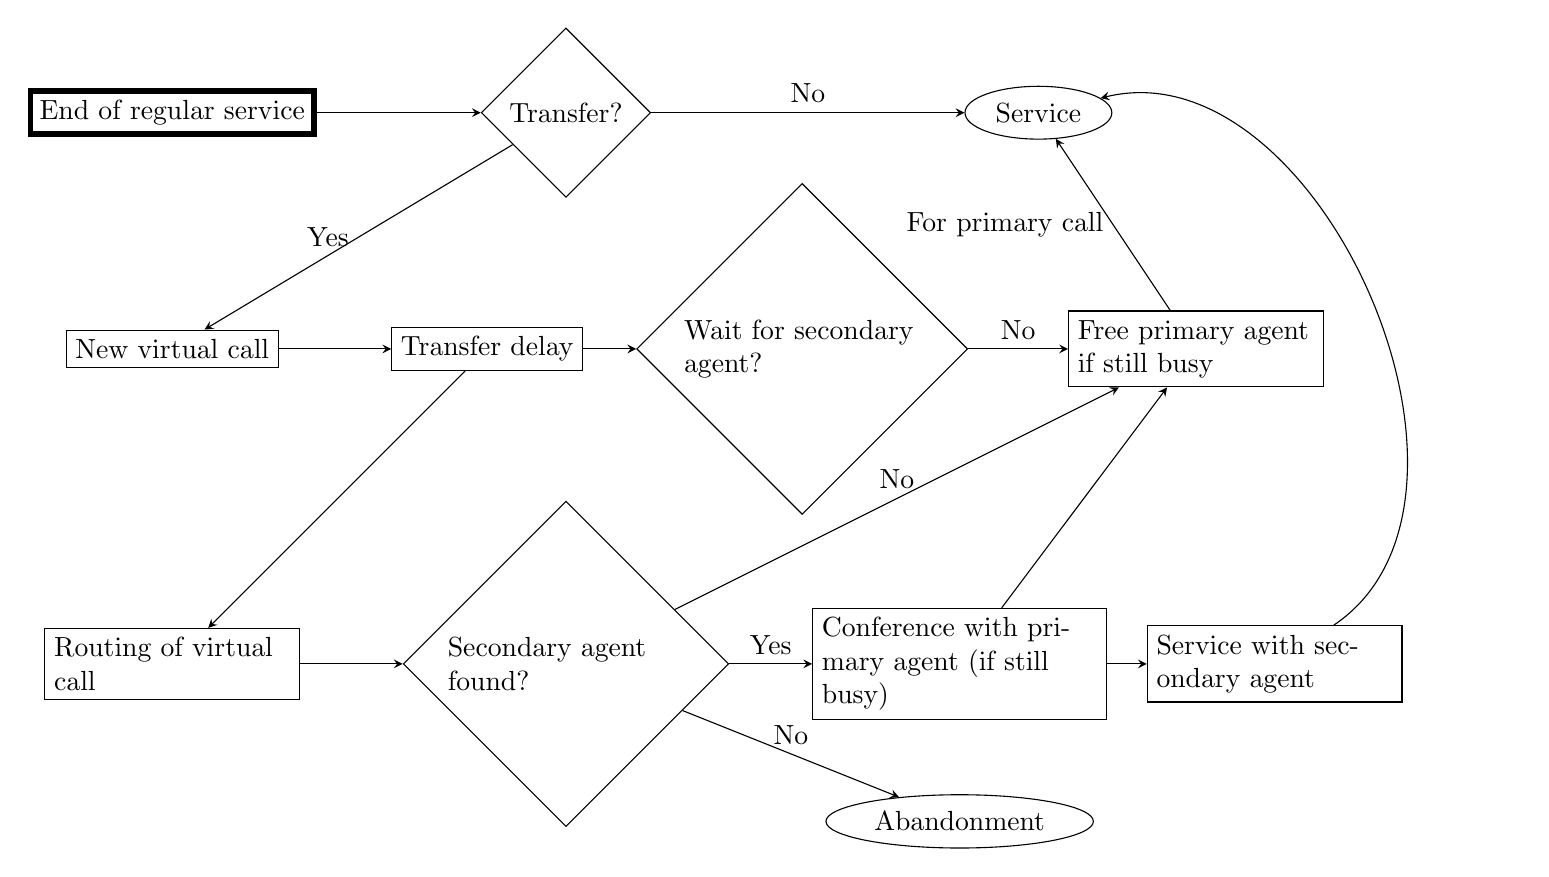
\begin{tikzpicture}[shape=rectangle,>=stealth]
\node (endService) [draw, line width=2pt] {End of regular service};
\node (transfer) [draw, shape=diamond, node distance=5cm, right of=endService]
{Transfer?};
\node (service) [draw, shape=ellipse, node distance=6cm, right of=transfer] {Service};
\node (virtualCall) [draw, node distance=3cm, below of=endService]
{New virtual call};
\node (transferDelay) [draw, node distance=4cm, right of=virtualCall]
{Transfer delay};
\node (transferWait) [draw, node distance=4cm, shape=diamond, right
of=transferDelay, text width=3cm]
{Wait for secondary agent?};
\node (freePrimary) [draw, node distance=5cm, right of=transferWait,
text width=3cm]
{Free primary agent if still busy};
\node (routing) [draw, node distance=4cm, below of=virtualCall, text width=3cm]
{Routing of virtual call};
\node (secondaryAgent) [draw, shape=diamond, node distance=5cm, right
of=routing, text width=3cm]
{Secondary agent found?};
\node (conference) [draw, node distance=5cm, right of=secondaryAgent,
text width=3.5cm]
{Conference with primary agent (if still busy)};
\node (service2) [draw, node distance=4cm, right of=conference, text width=3cm]
{Service with secondary agent};
\node (abandonment) [draw,shape=ellipse, below of=conference, node
distance=2cm]
{Abandonment};

\draw[->] (endService) -- (transfer);
\draw[->] (transfer)
edge
node [left] {Yes}
(virtualCall)
edge
node [above] {No}
(service);
\draw[->] (virtualCall) -- (transferDelay);
\draw[->] (transferDelay) -- (transferWait);
\draw[->] (transferWait)
--
node [above] {No}
(freePrimary);
\draw[->] (freePrimary) -- 
node [left] {For primary call}
(service);
\draw[->] (transferDelay) -- (routing);
\draw[->] (routing) -- (secondaryAgent);
\draw[->] (secondaryAgent)
edge
node [above] {Yes}
(conference)
edge
node [above] {No}
(freePrimary)
edge
node [above] {No}
(abandonment);
\draw[->] (conference) -- (freePrimary);
\draw[->] (conference) -- (service2);
\draw[->, bend angle=80] (service2) edge [bend right] (service);
\end{tikzpicture}


\caption{The transfer of a call to a secondary agent}
\label{fig:calltransfer}
\end{figure}

More specifically, transfer works as follows.
Let $C$ be a call of type~$k$ arrived during period~$p$,
and served by an agent $A$ in
group~$i$.
With probability $r_{k,i, p}$, the call is transferred to another
agent after service.
In that case, we suppose that the transfer decision
is taken before beginning of service, and
multiply the service time of the call to be transferred by $m_{k,i,p}$,
a constant depending on the call type, group of the serving agent, and
main period of arrival of the call.
Let $k'$ be the target random call type associated with call~$C$ for
the transfer.
This new type index is generated randomly from a discrete
distribution giving
call type $k'$ a probability $w_{k,p',k'}$ depending on $k$ and $p'$.

A new call of type $k'$ is  created, and
receives completely new attributes such as patience, and
service times.
This new call $C'$ is a virtual call corresponding to $C$.

A random delay depending on $k$, $i$, and
$p$ then occurs.  This delay, which is 0 by default, represents the time
spent by the agent $A$ to initiate the transfer, e.g., dialing a phone
number.
After the delay,
the new call $C'$ is sent to the router the same way as an ordinary call.
The router's policy can thus apply specific rules for
type~$k'$, which can differ from call type~$k$.

Then, with probability $1-q_{k, i, p}$, the agent $A$ is freed
although the transfer of the call is not finished; this
is sometimes called a \emph{cold transfer}.
On the other hand,
with probability $q_{k, i, p}$, agent~$A$ waits for call $C'$ to reach
a free secondary agent $B$, or abandons;
this is often denoted a \emph{warm transfer}.
In case of abandonment, calls $C$ and $C'$ end, and agent $A$ is
freed.
Note that call $C$ is counted as a served call, even though $C'$
abandons.

If service of call $C'$ begins, and agent $A$ is still waiting, a
random conference time depending on
type $k'$, period of transfer $p'$, and secondary agent group $i'$ is
generated.
If this conference time is greater than 0, it adds up to the regular
service time of call $C'$ (i.e., service time is increased), and agent
$A$ waits for the conference time.
Note that the conference time is part of the service time both for
call $C$, and call $C'$.

If service of call $C'$ begins, but agent $A$ is not waiting,
another random pre-service time occurs before the regular service
time.
This time can be used to model, e.g., a customer identification
process.

\subsection{Virtual queueing or call backs}

Some call centers make predictions of the waiting time of new
customers, and offer them the possibility to be called back at a later
time if the predicted waiting time is too long.
We also say that customers to be called back join a \emph{virtual
  queue} since the system must keep a record of such customers in
order to perform the callbacks.
Virtual queueing is modeled as shown on figure~\ref{fig:vqueue} in
the simulator.

\begin{figure}
\centering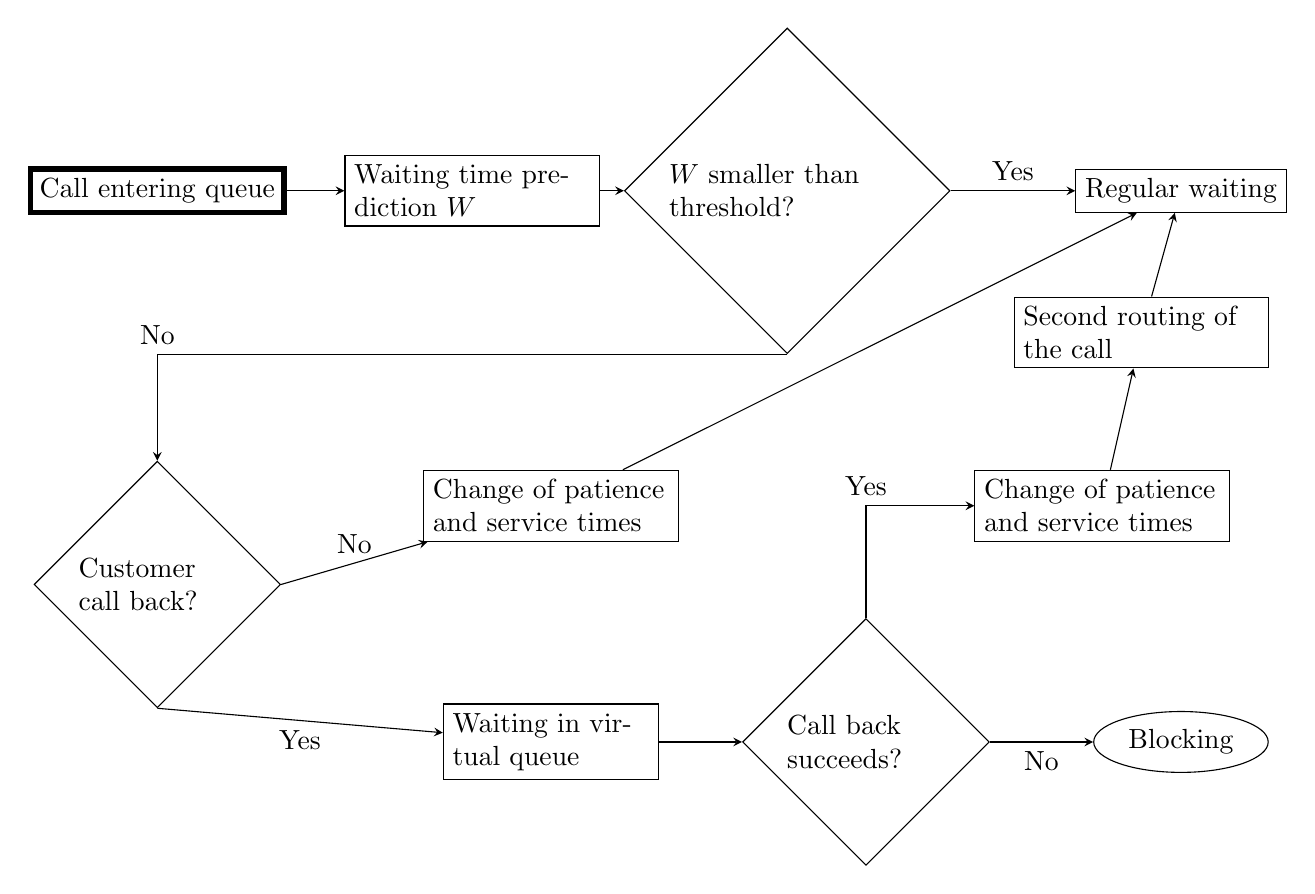
\begin{tikzpicture}[shape=rectangle,>=stealth]
\node (enterQueue) [draw, line width=2pt] {Call entering queue};
\node (wtPred) [draw, node distance=4cm, right of=enterQueue, text
width=3cm] {Waiting
  time prediction $W$};
\node (thresh) [draw, shape=diamond, node distance=4cm, right
of=wtPred, text width=3cm]
{$W$ smaller than threshold?};
\node (regWait) [draw, node distance=5cm, right of=thresh]
{Regular waiting};
\node (vqopt) [draw, shape=diamond, node distance=5cm, below
of=enterQueue, text width=2cm]
{Customer call back?};
\node (multnovq) [draw, node distance=5cm, right of=vqopt, text
width=3cm, yshift=1cm]
{Change of patience and service times};
\node (waitvq) [draw, node distance=3cm, below of=multnovq, text
width=2.5cm]
{Waiting in virtual queue};
\node (callback) [draw, shape=diamond, node distance=4cm,
right of=waitvq, text width=2cm] {Call back succeeds?};
\node (blocked) [draw, shape=ellipse, node distance=4cm,
right of=callback] {Blocking};
\node (multcallback) [draw, node distance=3cm, above of=blocked, text
width=3cm, xshift=-1cm] {Change of patience and service times};
\node (routing) [draw, node distance=2.2cm, above of=multcallback,
text width=3cm, xshift=0.5cm]
{Second routing of the call};

\draw[->] (enterQueue) -- (wtPred);
\draw[->] (wtPred) -- (thresh);
\draw[->] (thresh)
--
node [above] {Yes}
(regWait);
\draw[->] (thresh.south) -| node [above] {No} (vqopt.north);
\draw[->] (vqopt.east) -- node [above] {No} (multnovq);
\draw[->] (multnovq) -- (regWait);
\draw[->] (vqopt.south) -- node [below] {Yes} (waitvq);
\draw[->] (waitvq) -- (callback);
\draw[->] (callback.east) -- node [below] {No} (blocked);
\draw[->] (callback.north) |- node [above] {Yes} (multcallback);
\draw[->] (multcallback) -- (routing);
\draw[->] (routing) -- (regWait);
\end{tikzpicture}


\caption{Virtual queueing of a call}
\label{fig:vqueue}
\end{figure}

More specifically,
virtual queueing is allowed for a given call type $k$ by setting a
target type index $k'$ as well as a threshold
for the expected waiting time.
The index $k'$ is used to separate calls waiting in
regular queue from calls sent to a virtual queue
while the threshold is used to test if the predicted queueing delay is
sufficiently long for virtual queueing to be worthwhile.
When a call whose type allows virtual queueing arrives, an estimate of
its expected waiting time is obtained, using the last observed waiting
time before a service as a default heuristic.
If this prediction $W$ is smaller than a user-defined threshold
$W_{k,p}$, where $p$ is the index of the main period of the call's
arrival, the call is processed normally.

Otherwise, with probability $p_{k, p}$, the call exits the regular
queue,
and is sent to the virtual queue. This models the fact that the center
announces the predicted waiting time to the caller, and the
caller chooses to hang up and be called back at a later time.
The customer stays in the virtual queue for a fixed time given
by $Wm_{k, p}$, where $m_{k, p}$ is a user-defined multiplier
defaulting to 1.
With probability $1-p_{k, p}$, the customer refuses to be called back,
and waits in the normal queue.
However, the patience and service times of such a customer is
multiplied by
user-defined factors $f_{k, p}$ and $g_{k,i,p}$, respectively,
which default to 1.
For example,
a patience time multiplier greater than 1 can be used to model the
fact that customers knowing
their expected waiting time could be more patient than
customers ignoring that information.

Before a call enters the virtual queue,
its type identifier
switches from $k$ to $k'$.
When the customer leaves the virtual queue, call back occurs:
with probability $c_{k, p}$, call back succeeds and the call is sent
back to the router to get a free agent, or to be queued again,
hopefully for a smaller time than if the customer had waited on the
phone.  Of course,
the parameters of the routing policy can be different for call types
$k$ and $k'$. For example, calls of type $k'$ often have priority over
calls of type $k$.
With probability $1-c_{k, p}$, call back fails and the call returning
from the virtual queue is lost; it is counted as a blocked call in
statistical reports.

Note that any random variable associated with the call having switched
type for virtual queueing is not generated a second time, from the
distribution
corresponding to type $k'$; the original values for call type $k$ are
kept.
However, the patience and service times of calls returning from
virtual queue are
multiplied by factors $h_{k, p}$, and $i_{k, i, p}$, respectively.
This can be used, e.g., to model
the fact that called back customers are not ready to wait as long as
regular customers.

\subsection{Simulation experiments}
\label{sec:mskexpintro}

Once the model parameters are set up,
the simulator can perform experiments whose aim is to estimate
\emph{performance
measures} corresponding
to expectations
or functions of expectations. Estimation is made
using averages, or functions of averages, respectively.

Usually, one simulates the complete horizon of the model,
and collects the resulting estimates.
The experiment is repeated several times with different random numbers
in order to i.i.d.\ observations for computing
averages, functions of averages,
confidence intervals, etc., for estimated performance measures.
Without multiple replications, the estimators would be too noisy to be
useful.

Alternatively, one can concentrate on a single period of the
horizon, and simulate it as if its duration was infinite in the model.
The parameters of the model are then fixed for the whole
simulation, and the system is
simulated for a certain time, usually larger than the duration of the
considered period.
The simulator uses batch means
\cite{sLAW00a,iBUI05b} to
compute confidence intervals on performance measures.
See section~\ref{sec:mskexp} for more details about these two types of
experiments.

\subsection{Simulation output}
\label{sec:mskoutputintro}

After any experiment, the simulator generates a report containing
general information as well as statistics for estimated
performance measures.
More specifically,
the simulator computes many (random) quantities
on (constant) time intervals $[t_1, t_2]$ such as
the
number of calls processed by the router (arrived calls), the number of
served and
blocked calls, calls which have abandoned, etc.
It also evaluates the integrals of
the number of busy and working agents over the interval $[t_1, t_2]$,
for each agent group.
The time interval can be the whole simulation, a single period, etc.,
and statistics may be computed for several different intervals.

By default, a call arriving during period $p$ is counted in statistics
related to period~$p$, even if it exits the system during period~$p+1$.
However,
using the \texttt{per\-Period\-Collecting\-Mode} attribute in
experiment parameters, one can make the simulator count the calls in
the period they leave the system.

Statistics are collected for main periods only.
As a consequence,
if the statistical period of a call is the preliminary or wrap-up
period, the call is not counted.
Without this restriction, the time interval of a statistic on the
whole horizon would be random, and could change from replications to
replications.

Usually, a call is counted once.
If a call switches from type $k$ to $k'$ due to virtual queueing, it
is counted as a type-$k'$ call when call back fails, or at abandonment
or end-service time.
However, when a call is transferred to another agent, the call served
with the primary agent is counted separately from the virtual call
produced by the transfer.

A performance measure on a time interval $[t_1, t_2]$
can concern a segment of call types~$k$, a segment
of agent groups~$i$, or a pair $(k, i)$.
Here, a segment is simply a set regrouping call types or agent groups.
Let $K'$ be the number of
segments of call types.
For more information about segments,
see
sections~\ref{javadoc:umontreal.iro.lecuyer.contactcenters.app.PerformanceMeasureType}
to~\ref{javadoc:umontreal.iro.lecuyer.contactcenters.app.ColumnType}.

\begin{comment}
Segments $k=0,\ldots,K-1$ are elementary, i.e., they
contains a single call type~$k$.
If $K>1$, segment $K'-1$ regroups all the $K$ call types.
The remaining $K'-K-1$ segments are user-defined and
therefore optional.
Usually, call types in a
user-defined segment share common properties, i.e., they
can originate from the same region,
corresponding callers can speak the same
language, etc.
If $K\le 1$, we have $K'=K$, and at most one elementary segment
exists;
no user-defined segments are allowed.

In a similar way, let $\Ki'$ be the number of
segments of inbound call types, $\Ko'$ the number of
segments of outbound call
types, and $I'$ the number of
segments of agent groups.

Also let $P'$ be the number of segments of time periods.
User-defined groups of periods can be used, e.g., to represent the
morning, a day in an horizon spanning a week, etc.
\end{comment}

% The same way as for call types and agent groups, users can define
% segments regrouping periods, so let $P'$ be the total number of main
% periods plus the number of segments regrouping main periods.
% A segment of periods might represent the morning, the afternoon, or an
% entire day for a time horizon spanning multiple days.

Random variables concerning a fixed time interval
can be regrouped into a
random vector $\boldX(t_1, t_2)\in\RR^d$.
The expectation $\E[\boldX(t_1, t_2)]$ is a vector of $d$ possible performance measures
which can be estimated by a vector of averages
$\bar\boldX_n(t_1, t_2)$.

Other performance measures can be defined using
functions $g:\RR^d\to\RR$, and correspond to functions of expectations
$g(\E[\boldX(t_1, t_2)])$ estimated using
functions of averages
$g(\bar\boldX_n(t_1, t_2))$.
For example, by dividing the average sum of waiting times
by the average number of arrivals, we obtain the
long term average waiting time over all calls
which estimates the long term expected waiting time.
Dividing the average number of busy agents by the average number of
agents gives the long term agents' occupancy ratio.

% Counts can be divided by the length of this
% interval to get normalized values also called rates.
% All these outputs estimate possible performance measures.

Another important performance measure is the service level
defined as follows.
Let $\Sg[k,p](s_{k,p})$ be the number of contacts served
after a waiting time less than or equal to $s_{k,p}$,
in inbound type segment~$k$, and
counted in period segment~$p$. Let
$S_{k,p}$ be the total number of served contacts
in inbound type segment~$k$
counted in period segment~$p$.
The constant $s_{k,p}$ is the \emph{acceptable waiting time}, and can
depend on $k=0,\ldots,\Ki'-1$ and $p=0,\ldots,P'-1$.
Also let $\Lg[k,p](s_{k,p})$ be
the number of contacts
in inbound type segment~$k$, counted in period segment~$p$, and
having abandoned after a waiting time smaller than
or equal to the acceptable waiting time, and $A_{k,p}$ be the
total number of arrivals, for inbound type segment $k$, and period
segment~$p$.
The \emph{service level} for inbound type segment~$k$,
and period segment~ $p$ is defined as
\[g_{1,k,p}(s_{k,p})=\frac{\E[\Sg[k,p](s_{k,p})]}{\E[A_{k,p} - \Lg[k,p](s_{k,p})]}.\]
Other definitions are possible for the service level, e.g.
\[g_{2,k,p}(s_{k,p})=\frac{\E[\Sg[k,p](s_{k,p}) + \Lg[k,p](s_{k,p})]}{\E[A_{k,p}]}.\]

% The acceptable waiting time
% depends on the inbound call type, and the time interval of the
% performance measure.
% If the time interval of a performance measure corresponds to
% main period~$p$,
% the threshold is $s_{k, p}$
% if the performance measure
% concerns call type~$k$, or $\sP{p}$ if it concerns all call types.
% For a measure concerning all periods, the thresholds
% are $\sK{k}$ for call type~$k$, or $s$ for all call types.

To make reporting easier,
related  performance
measures are regrouped into
matrices whose rows represent segments of
contact types or agent groups, and whose
columns usually represent time intervals.  In some situations, there is a
single period, which results in single-column matrices.
For example, the expected number of served calls of each
type, and for each period, estimated by averages, is such a group of
performance measures.
%The integral of the queue size for each waiting queue,
%is computed during simulation for estimating
%time-average queue sizes, another group of performance measures.

Many other performance measures can be estimated by the simulator.
See
section~\ref{javadoc:umontreal.iro.lecuyer.contactcenters.app.PerformanceMeasureType}
for a complete list of supported performance measures.
See also section~\ref{sec:mskoutput} for more information about how
confidence intervals are computed, and the contents and possible
formats of statistical reports.

\begin{comment}
\subsubsection{Choosing the time interval of an event}

When time intervals
correspond to the periods of the horizon, events concerning a call are
counted in
the statistical period associated with that call.
This usually corresponds to the period of arrival.
On the other hand, when the intervals correspond to batches (see
section~\ref{sec:expsteadystate}) in the context
of a simulation on an infinite horizon, all events concerning a call are
counted in the batch the call leaves the system.

% To estimate the \emph{service level}, i.e., the proportion of calls
% served before a maximal waiting time, each inbound call type has an
% associated
% \emph{acceptable waiting time} $\sK{k}$.
% The model uses a global
% acceptable waiting time $s$ to estimate the overall service
% level.  $\sP{p}$ is defined as the acceptable waiting time for all call
% types and period~$p$ whereas $s_{k, p}$ is defined to be the
% acceptable waiting time for call type~$k$ and period~$p$.  For each
% obtained service level, thresholds $\lK{k}$, $l$, $\lP{p}$, $l_{k, p}$
% are defined to be used by
% optimizers to establish constraints over the service level.
\end{comment}

\subsection{The simplified CTMC model}

Simulation-based optimization requires many replications to evaluate
the performance of a call center for different configurations, e.g.,
with different staffing vectors.
With the generic multi-skill and blend simulator using the model
described here, this is often too CPU intensive.
The commonly used approximation formulas to work around this problem
oversimplify reality.
An alternative simulator using a simplified continuous-time Markov chain
(CTMC) model is thus
provided.
This simulator generates transitions using the embedded discrete-time
Markov chain (DTMC), and computes expectations conditional to the
sequence of visited states.

The CTMC model used by this simulator is similar to the model
described in this section, with the following simplifications.
First, arrivals always follow the Poisson process, patience and times are
exponential, there is no outbound call, no virtual queueing, no call
transfer, and agents cannot disconnect after service termination.
Moreover, the queue capacity is always finite.

The following routing policy is used to select an agent for a new call.
Each call type~$k$ has a list
$I_{k, 0}, I_{k, 1}, \ldots$, where $I_{k,j}$ is a set of
agent groups, for $j=0,\ldots$.
When a call of type~$k$ arrives,
if at least one free agent is available in one of the groups in $I_{k,0}$,
the call is sent to a free agent in the group of $I_{k,0}$ containing the
greatest number of free agents.
If several groups $i\in I_{k,0}$ contain the same maximal number of free
agents, the group with the maximal number of free agents, and
the smallest index $i$ is taken.
On the other hand, if no group in $I_{k,0}$ contains free agents, the
sets $I_{k,1}$, $i_{k,2}$, etc.\ are tested in a way
similar to $I_{k,0}$, in the order given by the list,  to
choose the first set with an agent group containing at least one free agent.
The sets $I_{k,j}$ are constructed from the matrix of ranks given by
the user. In particular,
the set $I_{k,0}$ is constructed by taking each agent group $i$ with the
minimal rank $\rTG(k,i)$.
The set $I_{k,1}$ is created by taking groups $i$ with second smallest
rank $\rTG(k,i)$.

For the selection of call at the end of service, each agent group has
a list
$K_{i,0}, K_{i,1}, \ldots$ of sets of call types.
First, if one waiting queue in $K_{i,0}$ contains at least one call,
the service starts
for the call having spent the greatest number of DTMC transitions in
queue, among calls in queues of $K_{i,0}$.
If more than one call spent the greatest number of transitions in queue,
the call with the greatest number of transitions in queue and
the smallest index $k$ is taken.
On the other hand, if no queue in $K_{i,0}$ contains calls,
the sets $K_{i,1}$, $K_{i,2}$, etc.\ are checked in a way
similar to $K_{i,0}$, in the order given by the list, to find the
first set with a queued call.
In a way similar to $I_{k,j}$, the sets $K_{i,j}$ are constructed by
using the values $\rGT(i,k)$ taken from the matrix of ranks given by
the user.

\section{Examples of data files}
\label{sec:mskconfig}

The configuration of the simulator is specified by at least two XML files.
A XML \cite{iYER04a} file contains a hierarchical structure of elements with
possible attributes and nested contents.
% The XML format only defines the syntax of the document, i.e., how
% contents must be formatted, while the author
% is free to use its own set of allowed elements, attributes, and nested
% contents.
% However, for XML files to be useful by programs, the author must
% conform to a
% determined \emph{schema} corresponding to a set of rules
% specifying acceptable contents.  The generic simulator we
% describe here
% uses such a schema for the definition of the parameters of call
% centers, and
% a second schema for experiment parameters.
% These schemas are described using a language called XML Schema
% \cite{iSPE00a}, and can be used to validate the contents of documents.
An overview of XML and data structures supported by the simulator
is provided in Section~\ref{sec:xmloverview}.

The first file specifies the parameters for the call center
itself.  These parameters are usually determined by a manager based on a
real system.  The second file specifies parameters for the simulation
experiment, such
as the simulation length, the required target relative error, etc. These
parameters are determined by the simulation expert at the time
experiments are performed.
Two formats are available for encoding parameters describing
experiments: a first one for the batch means
method and a second one for simulation using independent
replications.

In this section, we present examples of parameter files for
different models of call centers.  We start with a single queue, and
extend it by adding a new call type, a new agent group, etc.
% The two following examples are
% single-period call centers intended to be simulated with batch means.
% The third example is a non-stationary multi-skill model with inbound
% types only.
The last examples are blend call centers
with one inbound call type and one outbound call type.  The last
example is a blend and multi-skill call center demonstrating most of
the possibilities of the simulator.

\subsection{Single queue}
\label{sec:singlequeue}

This example models
a call center with a single call type, a single agent group, but
multiple time periods.
Each day, the center operates for $P$ hours.
The parameters can change during the day, but
they are constant within each hour.

Calls arrive following a Poisson process with piecewise-constant
arrival rate $\lambda_p$ during period~$p$, where
$\lambda_p$ is
constant.
Calls that cannot be served immediately are put in a FIFO queue,
and abandon
if they wait more than their patience time.  The i.i.d.\ patience
times are generated as follows: with probability $\rho$, the patience
time is 0, i.e., the caller abandons if he cannot be served
immediately.  With probability $1-\rho$, the patience time is
exponential with mean $1/\nu$.  Service times are i.i.d.\ exponential random
variables with mean $1/\mu$.

During main period~$p$, $N_p$ agents are available to serve calls.
If, at the end of period~$p$, the number of busy agents is
larger than $N_{p+1}$, ongoing calls are completed, but new
calls are not accepted until the number of busy agents is smaller than
$N_{p+1}$.  During the preliminary period, there is no agent whereas
for the wrap-up period, $N_{P+1}=N_P$.
Listing~\ref{par:singleQueue} presents the XML file for this example.

\lstinputlisting[caption={\texttt{singleQueue.xml}: Example of
 parameter file for a call center with a single queue}, language=XML%
,label=par:singleQueue]{singleQueue.xml}

The XML file presented here is composed of elements and attributes
describing the hierarchical data.
In a XML document, \emph{elements} are used to represent complex
data.  Each element has a tag name, e.g., \texttt{serviceTime},
opening and closing markers (e.g.,
\lstinline[language=XML]{<serviceTime>},
and \lstinline[language=XML]{</serviceTime>}),
a set of attributes, and nested contents.
An \emph{attribute} is a key-value pair representing simple data
associated to an element
while \emph{nested contents} can be simple text or children elements.
Each document has a single \emph{root element} which can have
an arbitrary number of attributes and children.
See Section~\ref{sec:mskxml} for more information.
The elements of any XML document can be represented as a tree
such as the one displayed on figure~\ref{fig:singleQueue}.
The figure shows that \texttt{MSKCCParams} is the root of the tree,
and has one child for the inbound call type, one child for the agent
group, etc.
We now describe the XML file in more details.

\begin{figure}
\centering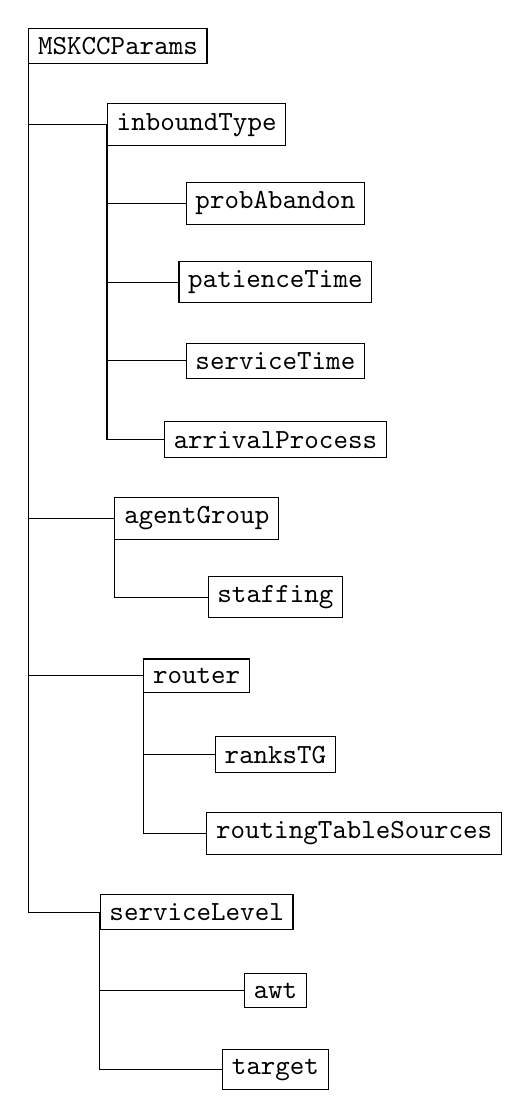
\begin{tikzpicture}[shape=rectangle,anchor=west]
\node (MSKCCParams) [draw] {\texttt{MSKCCParams}};
\node (inboundType) [draw, below of=MSKCCParams, xshift=1cm]
{\texttt{inboundType}};
\node (probAbandon) [draw, below of=inboundType, xshift=1cm]
{\texttt{probAbandon}};
\node (patienceTime) [draw, below of=probAbandon]
{\texttt{patienceTime}};
\node (serviceTime) [draw, below of=patienceTime]
{\texttt{serviceTime}};
\node (arrivalProcess) [draw, below of=serviceTime]
{\texttt{arrivalProcess}};
\node (agentGroup) [draw, below of=arrivalProcess, xshift=-1cm]
{\texttt{agentGroup}};
\node (staffing) [draw, below of=agentGroup, xshift=1cm]
{\texttt{staffing}};
\node (router) [draw, below of=staffing, xshift=-1cm]
{\texttt{router}};
\node (ranksTG) [draw, below of=router, xshift=1cm]
{\texttt{ranksTG}};
\node (routingTableSources) [draw, below of=ranksTG, xshift=1cm]
{\texttt{routingTableSources}};
\node (serviceLevel) [draw, below of=routingTableSources, xshift=-2cm]
{\texttt{serviceLevel}};
\node (awt) [draw, below of=serviceLevel, xshift=1cm]
{\texttt{awt}};
\node (target) [draw, below of=awt]
{\texttt{target}};

\draw (MSKCCParams.west) |- (inboundType)
(MSKCCParams.west) |- (agentGroup)
(MSKCCParams.west) |- (router)
(MSKCCParams.west) |- (serviceLevel);
\draw (inboundType.west) |- (probAbandon)
(inboundType.west) |- (patienceTime)
(inboundType.west) |- (serviceTime)
(inboundType.west) |- (arrivalProcess);
\draw (agentGroup.west) |- (staffing);
\draw (router.west) |- (ranksTG)
(router.west) |- (routingTableSources);
\draw (serviceLevel.west) |- (awt)
(serviceLevel.west) |- (target);
\end{tikzpicture}


\caption{The hierarchical structure of example in Listing~\ref{par:singleQueue}}
\label{fig:singleQueue}
\end{figure}

For call center parameters,
the name of the root element must be
\texttt{MSKCCParams}
%(see
%section~\ref{javadoc:umontreal.iro.lecuyer.contactcenters.msk.CallCenterParams})
with a namespace URI set to
\path{http://www.iro.umontreal.ca/lecuyer/contactcenters/msk}.
The \texttt{xmlns:ccmsk} attribute of this root element is used to
bind this URI to the shorter prefix \texttt{ccmsk} in the parameter
file.

The root element
is allowed to have some attributes such as
\texttt{period\-Duration} (main period duration
$d$),
%see p.~\pageref{javadoc:umontreal.iro.lecuyer.contactcenters.msk.CallCenterParams:getPeriodDuration()})
%and \texttt{queue\-Capacity} (maximal number of calls in queue) %, see
%p.~\pageref{javadoc:umontreal.iro.lecuyer.contactcenters.msk.CallCenterParams:getQueueCapacity()}),
\texttt{defaultUnit} (default time unit), etc.,
as well as children elements.
The attributes of an element are given after the name of the element,
and before the \texttt{>} marker.
Nested contents of the root element
is located between the
\lstinline[language=XML]!<ccmsk:MSKCCParams>!
and \lstinline[language=XML]!</ccmsk:MSKCCParams>! markers.

In this model, 13 periods of one hour are set up by setting
\texttt{num\-Periods} to 13 and \texttt{period\-Duration} to
\texttt{PT1H}.
The notation for time durations, which seems confusing at first
sight, is imposed by the XML Schema Specification (see
Section~\ref{sec:simpledatatypes}, and \cite[part 2, section
3.2.6]{iSPE00a}).
%The period
%duration must be set although it
%is unused for a stationary simulation, and conforms to the
%\texttt{duration} type defined by XML Schema .

The attribute
\texttt{default\-Unit},
%(see~p.~\pageref{javadoc:umontreal.iro.lecuyer.contactcenters.msk.CallCenterParams:getDefaultUnit()}),
set to \texttt{SECOND} in this example, sets the implicit unit
for time
durations.
This is the time unit used during simulation as well as the unit of
any time-related output, e.g., waiting time.

Nested elements are used to describe more complex information such
as call types, agent groups, the router, and the parameters
for estimating the service level.
The order of these elements must not be changed for the parameter file
to remain valid.
It is also important to keep the hierarchy of the document, e.g.,
the \texttt{router} element should not be moved inside an
\texttt{inbound\-Type} element.

We now describe the contents of the \texttt{inbound\-Type} element,
which represents the call type in this example, in more details.
First, the \texttt{name} attribute is used to bind a name to the
inbound call type.  A name can also be associated with an agent group.

The \texttt{prob\-Abandon} element is used to set the
probability of balking, for each main period.
This element accepts an array of values on the $[0,1]$ interval.
If the array contains a single value such as in this example, the
value is automatically reused for all
periods.  Therefore, the user does not need to repeat $0.1$ 13 times
to have $\rho=0.1$ for all periods in this example.

The way patience and service times are specified differ from the way
the period duration is given, because these aspects of the model
require probability
distributions, not only mean time durations.
The distribution for patience time is given using the
\texttt{patience\-Time} element
% (see
%p.~\pageref{javadoc:umontreal.iro.lecuyer.contactcenters.msk.CallTypeParams:getPatienceTime()})
whose type corresponds to a probability distribution.
% (see
%section~\ref{sec:probdist}).
  Such an element
accepts a
\texttt{distribution\-Class} attribute giving the SSJ class of the
probability distribution while the \texttt{default\-Gen} child element
sets the distribution parameters.
The latter element accepts an array giving
the arguments passed to the constructor of the chosen
distribution class.
The role of these arguments depends on the chosen distribution class,
and do not always correspond to means and variances.

Table~\ref{tab:maindist} gives the parameters for the
most commonly used distributions.
The first column gives the name of the class, i.e., the value of the
\texttt{distribution\-Class} attribute, corresponding to the
distribution.
The other columns give the density of the distribution, its
mean, its variance, and
the
order of parameters required for the
distribution.
See the package \path{umontreal.iro.lecuyer.probdist}
in the
user's manual of SSJ \cite{iLEC04j} for additional distributions.

\begin{table}
\caption{Parameters for the most commonly used probability distributions}
\label{tab:maindist}

\begin{center}
\begin{tabular}{|l|l|l|l|l|}\hline
\texttt{distributionClass} & Density $f(x)$ & Mean & Variance & Parameters \\ \hline
\texttt{ExponentialDist} & $\lambda e^{-\lambda x}$ for $x\ge
0$& $1/\lambda$ & $1/\lambda^2$ &
$\lambda>0$ \\
\texttt{ExponentialDistFromMean} & $e^{-x/\mu}/\mu$ for $x\ge
0$& $\mu$ & $\mu^2$ &
$\mu>0$ \\
\texttt{GammaDist} & $\lambda^{\alpha} x^{\alpha -
  1}\frac{e^{-\lambda x}}{\Gamma(\alpha)},$
for $x>0$ & $\alpha/\lambda$ & $\alpha/\lambda^2$ &
$\alpha>0$, $\lambda>0$ \\
\texttt{GammaDistFromMoments} &
 & $m$ & $v$ &
$m>0$, $v>0$ \\
\texttt{NormalDist} &
$\frac{\exp(-(x-\mu)^2/(2\sigma^2))}
         {\sqrt{2\pi}\sigma}$ &
$\mu$ & $\sigma^2$ &
$\mu$, $\sigma>0$ \\
\texttt{LognormalDist} &
  $\frac{\exp(-(\ln (x) - \mu)^2/(2\sigma^2))}{\sqrt{2\pi}\sigma x}$,
      &$e^{\mu+\sigma^2/2}$ & $e^{2\mu + \sigma^2}(e^{\sigma^2} - 1)$
& $\mu$, $\sigma>0$\\
&for   $x>0$
& && \\
\texttt{LognormalDistFromMoments}
& & $m$ & $v$ & $m>0$, $v>0$ \\
\hline
\end{tabular}
\end{center}

Here,
$    \Gamma (\alpha) = \int_0^\infty x^{\alpha-1} e^{-x} dx$.
In particular, $\Gamma(n) = (n-1)!$ when $n$ is a positive integer.

The gamma and lognormal distributions with moments have the same
density as the ordinary gamma and lognormal distributions, but a mean
and a variance are entered rather than shape and scale parameters.
\end{table}

According to Table~\ref{tab:maindist} or
the SSJ
documentation from \cite{iLEC04j}, the exponential
distribution is represented by the
\texttt{Exponential\-Dist\-From\-Mean} class,
and
has a scale parameter $\mu$ representing the mean
which needs to be
specified as an argument for calling the constructor.
%Since the \texttt{probdist} package was
%imported at the beginning of the XML file,
%the fully qualified class names of distributions do not need to be
%specified in \texttt{distribution\-Class} attributes.
Here,
$\mu=1000$.
The \texttt{unit} attribute of \texttt{patience\-Time} specifies that
the generated patience times must be considered in seconds, so
the mean patience time is 1000s for this example.
The \texttt{service\-Time} element % (see p.~\pageref{javadoc:umontreal.iro.lecuyer.contactcenters.msk.CallTypeParams:getServiceTime()})
has the same structure as
\texttt{patience\-Time}, but it gives the service time distribution for
calls, served by any agent.

The \texttt{arrival\-Process} element % (see Section~\ref{javadoc:umontreal.iro.lecuyer.contactcenters.msk.ArrivalProcessParams})
specifies the arrival process to
be used for this inbound call type, along with its parameters.
The \texttt{type} attribute is used to indicate the type of
arrival process, which can be any string specified in
Section~\ref{javadoc:umontreal.iro.lecuyer.contactcenters.app.ArrivalProcessType}.
The \texttt{arrivals} vector element gives the parameters for the
arrival process, in this case the Poisson arrival rate.
By default,
this arrival rate corresponds to the expected number of calls during a
simulation time unit, i.e., one second in our setting.
By setting the \texttt{normalize} attribute to \texttt{true}, we
instruct the simulator to interpret the arrival rates as relative to
one period.  Consequently, the given arrival rates set the expected
number of arrivals during each hour for this example.

The
\texttt{agent\-Group} element % (see Section~\ref{javadoc:umontreal.iro.lecuyer.contactcenters.msk.AgentGroupParams})
describes the agent group in the call
center.
The \texttt{staffing} child element is used to associate a staffing
with the agent group.
It contains an array giving the number of agents during each main
period of the day.
Alternatively, the array can contain a single element; the staffing
will then be fixed for the whole day.

Then, the \texttt{agent\-Group} element is used to describe the agent
group of the example.
We give a name to the agent group using the \texttt{name} attribute
and configure its staffing using the \texttt{staffing} element.
This gives a number of agents for each main period of the model.

The \texttt{router} element is then used to describe how routing is
done in the model.
Here, we have a very basic routing sending any incoming call to a free agent.
For this, the \texttt{router\-Policy} attribute is used to configure the
router's policy. Here, we use the \texttt{AGENTSPREF} policy which is
very general.
But we could use other more efficient policies for this example.
Section~\ref{javadoc:umontreal.iro.lecuyer.contactcenters.app.RouterPolicyType}
describes in details the
available router's policies.

The selected router's policy minimally requires a
$K\times I$ matrix associating a
priority to each (call type, agent group) pair during agent selection,
and
a second $I\times K$
matrix setting the priorities similarly during call
selection.
The first matrix is set using \texttt{ranksTG} (ranks for
type-to-group assignments)
while the second matrix is given using \texttt{ranksGT}
(ranks for group-to-type assignments).
A matrix can be represented by a sequence of arrays in the parameter
file, each array being represented by a \texttt{row} child element.
Here, we use the $1\times 1$ identity matrix for both parameters.
The second matrix can be given explicitly using the
\texttt{ranksGT}.
However, instead of transposing the contents of
\texttt{ranksTG} manually to obtain
\texttt{ranksGT} when $\rTG(k,i)=\rGT(i,k)$ for
all $k$ and $i$, we can instruct
the router to generate \texttt{ranksGT} by
transposing \texttt{ranksTG},
by using the \texttt{routing\-Table\-Sources} element.
This will become useful when we increase the number of call types and
agent groups.

The \texttt{service\-Level} element
%(see Section~\ref{javadoc:umontreal.iro.lecuyer.contactcenters.app.ServiceLevelParams})
gives thresholds for the service level using
two $\Ki'\times P'$
matrices: one for the acceptable waiting times, and a second one for the service
level targets.  Often, $\Ki'=\Ki+1$ if $\Ki>1$, and $\Ki$ otherwise,
and $P'$ is defined similarly using $P$.
Several \texttt{service\-Level} elements, with different
\texttt{awt} and \texttt{target} matrices, can
be specified to set the values for different contact types and
periods.
The targets are not considered during
simulation, but they can be used by
optimization programs.

However, these matrices are sometimes sparse, i.e., the user only
specifies some values.  Consequently, if a matrix of thresholds (or targets)
contains a single element, its single value is used for all call
types and periods.  If it contains a single row or column, the row or
column is duplicated as required.

Here, we set the acceptable waiting time to 20s, and the service level
target to 80\%.
We need $1\times 1$ matrix containing \texttt{PT20S}, and
\texttt{0.8}, respectively.
We also specify a second threshold of 30s with target 80\% by using a
second \texttt{service\-Level} element.

After the model parameters are configured, simulation parameters are
needed in order to perform experiments.
The simplest method of experiment consists of simulating a fixed
number of independent replications.  This can be described by a file
similar to
Listing~\ref{par:repSimParams}.

\lstinputlisting[caption={\texttt{repSimParams.xml}: Example of a
  parameter file for an
  experiment using independent replications}, language=XML%
,label=par:repSimParams]{repSimParams.xml}

The root element for the parameter file is \texttt{rep\-Sim\-Params} %(see
%Section~\ref{javadoc:umontreal.iro.lecuyer.contactcenters.app.RepSimParams}).
with namespace URI
\path{http://www.iro.umontreal.ca/lecuyer/contactcenters/app},
which differs from the namespace URI of \texttt{MSKCCParams}.
The number of performed runs is
fixed to 300 by the \texttt{min\-Replications}
attribute.

The \texttt{report} element % (see
%Section~\ref{javadoc:umontreal.iro.lecuyer.contactcenters.app.ReportParams})
contains the parameters of the statistical report produced by the
simulator.
In particular, the \texttt{confidence\-Level}
attribute sets the confidence
level of intervals to 95\%.
These confidence intervals are computed using the normal
assumption (see Section~\ref{sec:mskoutput}
for more details).
The report is printed when the simulator is invoked from the
command-line or when the \texttt{format\-Statistics} method is called
from a Java program.
This includes the confidence level of the printed intervals as well as
the statistics to include in the report.
Here, no information is provided about printed statistics so
the report includes information about all supported performance
measures.

\subsection{Variants of the single-queue model}

\subsubsection{Disabling abandonment}

In some situations, it can be necessary to disable abandonment, e.g.,
if no information about patience is available, or if simulation needs to
be compared with approximation formulas.
Doing this increases the workload of the simulated agents, because customers
abandoning must now all be served.
This increases the waiting time, and decreases the service level if
the number of agents is not increased to compensate for this.
Of course, a model without abandonment is less realistic than an
equivalent model with abandonment.

Abandonment can be disabled by
removing \texttt{prob\-Abandon} and \texttt{patience\-Time} from the
XML file.
Removing \texttt{prob\-Abandon} disables balking by setting the
probability of immediate abandonment to 0 while
removing \texttt{patience\-Time} sets all patience times to infinity.

Removing an element from a XML file can be performed by destructively
deleting all the text representing the element, and its children, or
by commenting it out. For example, the following code represents a
patience time which was commented out:
\begin{lstlisting}[language=XML]
<!--
      <patienceTime distributionClass="ExponentialDistFromMean" unit="SECOND">
         <defaultGen>1000</defaultGen>
      </patienceTime>
-->
\end{lstlisting}
The sequences \verb.<!--. and \verb.-->. serve as comment delimiters
in the XML language.  Since comments are ignored by the parameter
reader, they can be used to store additional information about the
parameter file.  This information is intended to be used by human
beings only.
Any information used by a computer program should be encoded in
XML elements, attributes, or nested text.

\subsubsection{Setting period-specific parameters}

The example on Listing~\ref{par:singleQueue} sets a stationary
distribution for the patience and service times.  If the distribution
of the service times can change from periods to periods, one can
replace the \texttt{default\-Gen} element of \texttt{service\-Time}
with a sequence of \texttt{period\-Gen} elements, as shown on the next
listing.
\begin{lstlisting}[language=XML]
      <serviceTime distributionClass="ExponentialDistFromMean"  unit="SECOND">
         <periodGen>100</periodGen>
         <periodGen>150</periodGen>
         <periodGen>180</periodGen>
         <periodGen>90</periodGen>
         <periodGen>110</periodGen>
      </serviceTime>
\end{lstlisting}
This sets the per-period mean service time, for a model defining five
main periods.
The $p$th \texttt{period\-Gen} element gives the parameters of the
service time for main period~$p$, with $p=1,\ldots,P$.
Of course, the number of \texttt{period\-Gen} elements must correspond
to the number of main periods in the model.

\subsubsection{Increasing the variability of arrivals}

\richard{Le d\'ebut de cette section doit \^etre r\'e\'ecrit pour tenir
compte de nos derni\`eres corrections: on peut inclure un facteur busyness
pour chaque type d'appel.}
With the arrival process of the original model, the number of arrivals
during period $p$ follows the Poisson distribution with mean
$\lambda_p$, and variance $\lambda_p$.
This variance can be increased randomizing the arrival rate in each
period.
The arrival process is then doubly stochastic.
For example, this can be done
by setting the arrival rates to
$B\lambda_p$, where $B$ is a random variable with mean 1.
The random variable $B$, generated each day,
represents the busyness factor of the day.
The day is more busy than usual when $B>1$ and less busy than usual
when $B<1$.
A well-studied distribution for $B$ is gamma with equal parameters
$\alpha_0$ \cite{ccAVR04a}.
Such a busyness factor can be used by adding the
\texttt{busyness\-Gen} element before any \texttt{inbound\-Type}
element, e.g.,
\begin{lstlisting}[language=XML]
   <busynessGen distributionClass="GammaDist">10 10</busynessGen>
\end{lstlisting}
This sets the distribution of the busyness factor to gamma(10,10).
This element does not accept \texttt{default\-Gen} or
\texttt{period\-Gen} children, because the busyness factor is
generated once at the beginning of the day, and thus does not change
from periods to periods.

Another way of increasing the variance of the number of arrivals is to
use a Poisson-gamma arrival process where the arrival rate for each
period is gamma-distributed, independently of other periods.
This can be specified as follows:
\begin{lstlisting}[language=XML]
      <arrivalProcess type="POISSONGAMMA" normalize="true">
         <poissonGammaShape>19 19 19 19 19 19 19 19
                            19 19 19 19 19</poissonGammaShape>
         <poissonGammaRate>100 150 150 180 200 150 150 150
                            120 100 80 70 60</poissonGammaRate>
      </arrivalProcess>
\end{lstlisting}
Here, we have changed the value of the \texttt{type} attribute to
\texttt{POISSONGAMMA}, and replaced the \texttt{arrivals} element
with \texttt{poisson\-Gamma\-Shape}, and
\texttt{poisson\-Gamma\-Rate}.
These new elements give the
gamma shape and rate parameters for each main
period.
Section~\ref{javadoc:umontreal.iro.lecuyer.contactcenters.app.ArrivalProcessType}
gives the list of all available arrival processes, with a detailed
description for each one.

\subsubsection{Changing the number of periods}

Increasing the number of periods often requires several updates in the
parameter file. First, the \texttt{num\-Periods} attribute in
\texttt{MSKCCParams} must be modified.
Then, each element defining period-specific parameters must be updated
with the new periods.
This includes balking probabilities
stored in \texttt{prob\-Abandon} elements,
patience and service times stored in
\texttt{patience\-Time} and \texttt{service\-Time} elements,
arrival process (\texttt{arrivals} elements for
Poisson processes with piecewise-constant rates), staffing
in \texttt{staffing} elements, and service
level information
in \texttt{service\-Level} elements.
Missing per-period parameters will result in error messages when
running the simulator.
If an element sets parameters for more periods than the value given by
\texttt{num\-Periods}, the last extra periods are ignored.
%TODO: print a warning in this case

\subsubsection{Adding a new call type}

Adding a new call type is a three-steps process:
\begin{enumerate}
\item Adding a new \texttt{inbound\-Type} element;
\item Adapting the routing policy for a new call type;
\item Extending the matrices of AWTs and targets for the service level.
\end{enumerate}
We now describe these steps in more details.

Adding a new \texttt{inbound\-Type} element can be done by copying the
contents of an existing \texttt{inbound\-Type} element, and
altering its contents.
The main issue to consider is the indexing of call types:
adding new call types can shift indices, and require adjustments in
other parts of the XML file.
More specifically, each call type receives an index based on its order
of occurrence in the XML file.
This index is used for specifying type-to-group and
group-to-type maps for some routing policies as well as
target call types for call transfers and virtual queueing.
See Section~\ref{sec:mskccParamsThreeTypes} for an example with a
type-to-group map.

In our original setting, the only call type has index 0.
Adding a new \texttt{inbound\-Type} element just below the original
one
creates a new call type with index 1.
However, adding the element \emph{before} the original
\texttt{inbound\-Type} element assigns index 0 to the new call type,
and shifts the index of the old call type to 1.
This can cause problems especially if the model already contains
several call types.

The second step in adding the call type is to update the parameters of
the routing policy.  In our example, we need to change
the
\texttt{ranksTG} child element of \texttt{router} in order to extend
the matrix of ranks with a new row.
This new row sets the priorities for the new
type.
Failing to do that will result in errors preventing the simulator to
run.

With a single agent group and
the agents' preference-based routing policy, if both call types have
the same priority,
agents becoming free select the call with the longest waiting time.
Otherwise, free agents first look for calls with the lowest rank
(i.e., highest priority) before calls with the highest rank.

If call type 1 has priority over call type 2, or even if
its mean service time is shorter than the mean service time of
call type 2,
calls of type~1 will wait less before they get service, and
therefore will have higher service level than
calls of type~2.

If both call types have the same priority, and mean service time, one
expects to get exactly the same results as with the model defining a
single call type.
In practice, results differ slightly because of the way random numbers
are generated by the simulator.
More specifically, sequences of random numbers are associated to each
call type separately.  By splitting the calls in two types,
one changes the number of constructed sequences of random streams, and
thus the generated random numbers.
Note that the difference between the single-type and the two-types model
decreases as the number of replications increases.

Extending matrices of AWTs and service level targets is optional if
it contains a single row, and the thresholds and targets do not depend
on the call type.
Otherwise, the matrices must contain one row per call type, plus a row
for the global parameters.

Listing~\ref{par:singleQueueTwoTypes} gives an example of a call
center with two call types, and one agent group.
Here, the target service level is 80\% for both types, but the AWT for
call type~2 is set to 60s.  The global AWT and target remain
at 20s, and 80\%, respectively.
In the new model, calls of type~1 have priority over calls of type~2.

\lstinputlisting[caption={\texttt{singleQueueTwoTypes.xml}: Example of
  a parameter file for a call center with a single agent group and two
call types}, language=XML%
,label=par:singleQueueTwoTypes]{singleQueueTwoTypes.xml}

\subsubsection{Adding a new agent group}
\label{sec:addAgentGroup}

Adding a new agent group involves two steps similar to adding a call
type:
\begin{enumerate}
\item Adding a new \texttt{agent\-Group} element;
\item Adapting the routing policy;
\end{enumerate}
We will now describe these steps in more details.

A new \texttt{agent\-Group} element can be added by copying an
existing element, and altering parameters.
Usually, the name and staffing of the agent group are adapted.
As with call types, adding agent groups can shift indices as we
discussed in the previous subsection.

The routing policy is adapted by adding a new column to
the matrix of ranks of the model.  This is done by updating the
\texttt{ranksTG} element in the parameter file.
This new column sets priorities concerning the new agent
group.
With a single call type, if two agent groups have the same priority,
a newly-arrived call is assigned to the agent with the longest idle
time among the two groups.
If ranks are different, the agent group with the lowest rank (i.e.,
highest priority) is checked for agents before the group with higher
rank.

Listing~\ref{par:singleQueueTwoGroups} gives an example of this
extension.  Here, we have added a second agent group, and set the
router for the first agent group to have priority over the second one.

\lstinputlisting[caption={\texttt{singleQueueTwoGroups.xml}: Example of
  a parameter file for a call center with two agent groups and a
single call type}, language=XML%
,label=par:singleQueueTwoGroups]{singleQueueTwoGroups.xml}

If we simulate with this parameter file, we obtain a warning about
agent groups not in detailed mode.  This is caused by the fact that in
general, the routing policy we have chosen requires the longest idle
times of agents to break tie for agent groups sharing the same minimal
rank.
This idle time can be obtained only when agent groups are in
detailed mode, i.e., if they model each agent as separate objects.
However, for this example, idle times are not needed, because all
ranks are different.

The warning can be removed two ways: by setting the
\texttt{detailed} attribute to \texttt{true}
for each \texttt{agent\-Group} element, or by
setting the \texttt{agent\-Selection\-Score} attribute of the
\texttt{router} element to something other than
\texttt{LONGESTIDLETIME}, e.g., \texttt{NUMFREEAGENTS}.
The first solution switches the agent groups to detailed mode, which
allows the idle times to be retrieved, while the second alternative
changes how tie is broken for agent groups sharing the same minimal
rank.

\subsubsection{Adding routing delays}

With the routing policy used in this model, agent groups are queried
sequentially in order to find a free agent to serve a newly-arrived
call; this is call \emph{overflow routing}.
Similarly, call types are looked up sequentially in order to find a
call for a free agent; this is denoted \emph{priority queueing}.
Sometimes, we need the router to wait for some time between each agent
group, and call type.  This can be done by setting delays in the
router's parameters.

First, the routing policy has to be switched from \texttt{AGENTSPREF}
to
\texttt{AGENTSPREFWITHDELAYS}.
Then, a $I\times K$ matrix of time durations is
specified using \texttt{delaysGT} element
Each element $(i, k)$ of the matrix gives the minimal time a call of
type~$k$ has to wait in queue before it can be served by any agent in
group~$i$.

As an example, suppose we combine the two extensions proposed in the
preceding subsections.  We therefore have two call types, and two
agent groups.
We then assign each call type $k=0,1$ a primary agent group $i$, but
we allow the other agent group to serve the call, with lower priority,
and a minimal delay of 30s.
The resulting \texttt{router} element looks as follows:
\begin{lstlisting}[language=XML]
   <router routerPolicy="AGENTSPREFWITHDELAYS">
     <ranksTG>
       <row>1   2</row>
       <row>2   1</row>
     </ranksTG>
     <delaysGT>
        <row> PT0S     PT30S</row>
        <row>PT30S      PT0S</row>
     </delaysGT>
     <routingTableSources ranksGT="ranksTG"/>
   </router>
\end{lstlisting}
Note that setting any rank for a $(k, i)$ pair
to $\infty$, by replacing the numerical
value with
\texttt{INF}, prevents the router from assigning
calls of type $k$ to agents in group $i$.

\subsubsection{Using agent schedules}
\label{sec:mskSchedules}

For any agent group described in a XML file representing call center
parameters, the staffing vector can be replaced with a schedule.
Schedules are composed of shifts to which
agents are assigned. The staffing vector is thus replaced with a vector
containing the number of agents per shift, with a description of the shifts.
The most common way of specifying schedule shifts is to give a
$J\times P$
matrix of booleans whose element $(j, p)$ is \texttt{true} if and only if
an agent working on shift $j$ is scheduled for main period~$p$.

Listing~\ref{par:singleQueueShifts} gives an example of an agent group
with a schedule. In this listing, the \texttt{staffing} element is
replaced with a \texttt{schedule} element containing a
\texttt{numAgents} child. This vector of agents instructs the simulator to
schedule one agent for each shift.
The matrix of shifts is set up using the element \texttt{shift\-Matrix}
which is placed after the element describing the agent group. Each row
of the matrix corresponds to a shift while each column concerns a main
period of the model.
The matrix of shifts is used for every agent group for which a schedule is
given.  Alternatively, one can give a matrix of shifts specific to an
agent group by putting a \texttt{shift\-Matrix} element inside the
\texttt{schedule} element, just before the \texttt{num\-Agents} element.

\lstinputlisting[caption={\texttt{singleQueueShifts.xml}: Example of
  a parameter file for a call center with a single agent group with
  a schedule, and a
single call type}, language=XML%
,label=par:singleQueueShifts]{singleQueueShifts.xml}

The simulator also accepts shifts represented as time
intervals. These are specified in the XML parameter file using
\texttt{shift} elements. For example, the first row of the
matrix of shifts in the above example may be written as follows.
\begin{lstlisting}[language=XML]
      <schedule>
         <shift numAgents="1">
            <shiftPart startingTime="PT8H" endingTime="PT12H" type="Working"/>
            <shiftPart startingTime="PT13H" endingTime="PT15H" type="Working"/>
         </shift>
      </schedule>
\end{lstlisting}
With this input method, the starting and ending times of shifts do not
need to match with a change of main period.

\subsubsection{Estimating parameters}
\label{sec:singleQueueMLE}

When modeling a call center, the probability
distributions of the random variables is unknown.
A common solution to this problem is to guess a parametric probability
distribution and fit real data to this distribution.
The generic simulator can estimate parameters from data for
probability distributions and some arrival processes by using
the maximum likelihood method.
For this, data can be specified directly in parameter files.
Listing~\ref{par:singleQueueMLE} presents the parameter file of the
example in Listing~\ref{par:singleQueue},
with some parameters replaced with artificial data.

\begin{lstlisting}[caption={\texttt{singleQueueMLE.xml}: Example of
  a parameter file with data for
  parameter estimation}, language=XML%
,label=par:singleQueueMLE]
<ccmsk:MSKCCParams defaultUnit="SECOND" periodDuration="PT1H"
                   numPeriods="13"      startingTime="PT8H"
     xmlns:ccmsk="http://www.iro.umontreal.ca/lecuyer/contactcenters/msk">
   <inboundType name="Inbound Type">
      <probAbandon>0.1</probAbandon>
      <patienceTime distributionClass="ExponentialDist" unit="SECOND">
         <defaultGen>0.001</defaultGen>
      </patienceTime>
      <serviceTime distributionClass="ExponentialDist" unit="SECOND">
     <!-- i.i.d. exponentials with lambda=0.01 -->
         <defaultGen estimateParameters="true">
   13.583  38.350  36.988  174.782  25.055  76.227  65.542  43.937
<!-- more observations here -->
</defaultGen>
      </serviceTime>
      <arrivalProcess type="PIECEWISECONSTANTPOISSON" normalize="true"
                      estimateBusyness="true">
        <!-- Observations generated from the Poisson distribution -->
         <data>
            <row>89 144 144 193 189 151 149 145 108 107 82 68 56</row>
            <row>93 153 166 173 175 173 137 158 110 86 73 74 53</row>
            <row>100 140 154 190 217 164 162 157 120 86 65 83 76</row>
            <row>99 153 155 143 222 146 151 157 125 89 81 58 66</row>
            <!-- More observations -->
         </data>
      </arrivalProcess>
   </inboundType>

   <agentGroup name="Inbound-only agents">
      <staffing>4 6 8 8 8 7 8 8 6 6 4 4 4</staffing>
   </agentGroup>

   <router routerPolicy="AGENTSPREF">
     <ranksTG>
       <row>1</row>
     </ranksTG>
     <routingTableSources ranksGT="ranksTG"/>
   </router>

   <serviceLevel>
      <awt>
         <row>PT20S</row>
      </awt>
      <target>
         <row>0.8</row>
      </target>
   </serviceLevel>
</ccmsk:MSKCCParams>
\end{lstlisting}

Data is specified at the same place as regular parameters, except that
the \texttt{estimate\-Parameters} attribute is set to \texttt{true}.
For probability
distributions over the real numbers (continuous or discrete), this
element is an array of double-precision values.
For discrete distributions over the integers, the double-precision
values of the data are rounded to the nearest integers.
%The \texttt{data} element can also be replaced by the \texttt{data\-URL}
%attribute which specifies the URL of a text file containing the data,
%one value per line.
%The URL can point to a local file, or a Web resource.
%Relative URLs are resolved using the location of the parameter file.
%Data can also be read from a CSV file or a database.
%See Section~\ref{sec:extarray} for more information.

For an arrival process, one must use the
\texttt{data} element which accepts a
matrix of integers giving the observed number of arrivals during each
main period for observed days.
The parameters of arrival processes are estimated by considering each
given
$P$-dimensional vector representing a day as independent and
identically distributed.

For arrival processes, parameter estimation is more complex, because
the number of arrivals in all periods comes from a multivariate
distribution, and some methods estimate the parameters of the busyness
factor and the arrival rates simultaneously.
For these reasons, the way parameters are estimated for arrival
processes depends on the specific type of process, and the value of
the \texttt{estimate\-Busyness} attribute.
For example, with the Poisson process with piecewise-constant arrival
rates, if the busyness factor is estimated, the number of arrivals is
assumed to follow the negative multinomial distribution, and a
gamma$(\alpha_0,\alpha_0)$ busyness factor is estimated.

Before the simulation starts, parameters are estimated using the
maximum likelihood method and used to create the
probability distributions; parameters are never displayed to the user.
If the results of the estimates need to
be known, a program is available to estimate parameters and produce a
new XML file representing the same model, with data replaced by
parameters.
See Section~\ref{sec:estparprg} for more information.

\subsection{Additional experiment parameters}

Listing~\ref{par:repSimParams} shows a very basic parameter file for
experiments with independent replications. By modifying
the \texttt{minReplications} and the \texttt{confidenceLevel}
attributes, we can change the number of replications to simulate and
the confidence level of intervals, respectively, but many other
parameters can be changed.  In this section, we give examples for the
most common changes.

\subsubsection{Getting a call-by-call trace}
\label{sec:trace}

Sometimes, it may be required to get a trace of every call processed
by the simulator.
This can be done by using the \texttt{call\-Trace} element in
experiment parameters as in Listing~\ref{par:repSimParamsTr}.
This parameter file indicates that 5 independent replications need to
be performed, and that a call-by-call trace has to be saved in the file
\texttt{test.log}.
The format of the trace file is plain text by default.
However, if one gives a file name ending with \texttt{.xls}, the trace
is stored into a spreadsheet compatible with Microsoft Excel.
Note that the \texttt{call\-Trace} element can also be used in
simulation parameters for batch means.

\lstinputlisting[caption={\texttt{repSimParamsTr.xml}: Example of a
  parameter file for an
  experiment using independent replications and producing a
  call-by-call trace}, language=XML%
,label=par:repSimParamsTr]{repSimParamsTr.xml}

%See
%Section~\ref{javadoc:umontreal.iro.lecuyer.contactcenters.app.CallTraceParams}
%for the exact contents of the trace.

\subsubsection{Restricting the printed statistics}

The \texttt{printed\-Stat} element % (see
%Section~\ref{javadoc:umontreal.iro.lecuyer.contactcenters.app.PrintedStatParams})
of \texttt{report}
indicates which performance measures
to print a report on.  During the simulation, statistics on all
supported performance measures are computed (see
Section~\ref{javadoc:umontreal.iro.lecuyer.contactcenters.app.PerformanceMeasureType}).
Listing~\ref{par:repSimParamsStat}
shows how to
indicate that we need a statistical report only for the
service level as well as the agents' occupancy ratio.  However, we do
not want a detailed report for the occupancy ratio: only the occupancy
ratio for all agent groups will be displayed.  But the
service level for each call type and period will be printed separately.
If no \texttt{printed\-Stat} element is given, a detailed report
for all supported performance measures is obtained.

\lstinputlisting[caption={\texttt{repSimParamsStat.xml}: Example of a
  parameter file for an
  experiment using independent replications and producing a report
  with selected statistics}, language=XML%
,label=par:repSimParamsStat]{repSimParamsStat.xml}

\subsubsection{Printing observations}

The simulator only computes statistics that do
not require the complete list of observations to be stored.
Consequently, observations are not stored in order to save memory.
However, in some situations, observations might be required, e.g.,
to estimate quantiles, plot histograms, etc.
The simulator therefore provides options to include observations for
selected performance measures into the generated report.
Measures have to be selected explicitly, because printing observations
for all measures would produce a huge report in which finding
the relevant information would be hard.

The list of observations are not available directly for performance measures
whose \texttt{EstimationType} is \texttt{FUNCTIONOFEXPECTATIONS}, as
for example \texttt{SERVICELEVEL}. For these, there is a closely related
performance measure with name suffix \texttt{REP},  of \texttt{EstimationType}
\texttt{EXPECTATIONOFFUNCTION}, for which the
complete list of observations may be collected by the simulator.
In the case of \texttt{SERVICELEVEL}, this measure is
\texttt{SERVICELEVELREP}.

Listing~\ref{par:repSimParamsObs} provides an example XML file for
printing observations.
First, the \texttt{keepObs} attribute has to be set to \texttt{true}
in order to instruct the simulator to keep observations.
Then, a \texttt{printedObs} element is added
for each performance measure for which observations are
desired.
The \texttt{row} and \texttt{column} attributes can be used to select
a specific row and column in the matrix of performance measures.
If they are omitted, observations are printed for the bottom-right
performance measure, which corresponds to the measure over all contact
types (or agent groups), and all time periods.

\lstinputlisting[caption={\texttt{repSimParamsObs.xml}: Example of a
  parameter file for an
  experiment using independent replications and producing a report
  with selected lists of observations}, language=XML%
,label=par:repSimParamsObs]{repSimParamsObs.xml}

Here, we select the number of served calls of any type,
the number of calls having abandoned,
and the number of calls of type 0 served after a waiting time
smaller than or equal to the acceptable waiting time.

\subsubsection{Changing random seeds}
\label{sec:seeds}

Although the simulation is stochastic, it always gives the same
results if it is performed with the same parameters.
This behavior is due to the fixed initial seed for random number
generators.
One can change this initial seed by using experiment parameters.
One can even use a different algorithm for generating uniform random
numbers.

For this,
the \texttt{random\-Streams} element is used to specify information
about random streams. In particular, the
optional \texttt{stream\-Seed} attribute allows one to set the
seed of random number generators for the simulation.  The value of
this attribute must correspond to an array given to the
\texttt{set\-Package\-Seed} static method of the selected random stream
class, \texttt{MRG32k3a} being the default.
These methods often take an array of integers as
argument.  With MRG32k3a, the default random number generator, one
needs an array of six integers to
represent the seed.
The optional attribute \texttt{stream\-Class} can be
used to specify a different class of random stream for generating
random numbers.  See the package \path{umontreal.iro.lecuyer.rng} in
the SSJ documentation \cite{iLEC04j} for more
information about available random streams.
Listing~\ref{par:repSimParamsSeed} gives an example of this.

\lstinputlisting[caption={\texttt{repSimParamsSeed.xml}: Example of a
  parameter file for an
  experiment using independent replications and different initial seed}, language=XML%
,label=par:repSimParamsSeed]{repSimParamsSeed.xml}

\subsubsection{Sequential sampling}

By default, the simulator performs a deterministic number of
replications set by the \texttt{min\-Replications} attribute, in
experiment parameters.
This becomes random if sequential sampling is used.
With this procedure, replications are performed until the target
relative error for selected performance measures falls below a
user-specified threshold.
More specifically, the simulator performs the minimal number of
replications, evaluates the relative error by dividing the half-width
of the confidence intervals by the point estimators, and estimates a
number of additional observations to generate.
This procedure continues until the relative error is smaller than the
targets for all selected performance measures, or a maximal number of
replications is reached.

Listing~\ref{par:repSimParamsSeqSamp} gives an example of a parameter
file for sequential sampling. Here, the element
\texttt{sequential\-Sampling} is used to select
performance measures for sequential sampling.
The \texttt{measure} attribute selects the service level as a group of measures.
For each main period of the model, we require that the relative error on
the service level be smaller than or equal to $1\%$, so the
attribute \texttt{target\-Error} is fixed to 0.01.
Confidence level on intervals used to estimate the relative errors are
computed with level given by the \texttt{confidence\-Level} attribute,
which can differ from the confidence level used for reporting.
Note that by setting the \texttt{global\-Only} attribute to
\texttt{true} in the \texttt{sequential\-Sampling} element, one could
select the overall service level only for sequential sampling rather
than the service level for all individual periods.

\lstinputlisting[caption={\texttt{repSimParamsSeqSamp.xml}: Example of a
  parameter file for an
  experiment using independent replications and sequential sampling}, language=XML%
,label=par:repSimParamsSeqSamp]{repSimParamsSeqSamp.xml}

\subsubsection{Parameters for the CTMC simulator}

The simplified CTMC simulator requires some additional parameters, for
example the length of the horizon used if simulating a single period.
Therefore, a parameter file similar to
Listing~\ref{par:repSimParamsCTMC} is needed.
A basic parameter file for the CTMC simulator is very similar to
regular files, except that an element with name
\texttt{ctmcrep\-Sim\-Params} rather than \texttt{rep\-Sim\-Params} is
used.
However, the \texttt{ctmcrep\-Sim\-Params} supports attributes and
child elements not supported by \texttt{rep\-Sim\-Params}.

\lstinputlisting[caption={\texttt{repSimParamsCTMC.xml}: Example of a
  parameter file for an
  experiment using independent replications and CTMC simulator}, language=XML%
,label=par:repSimParamsCTMC]{repSimParamsCTMC.xml}

In Listing~\ref{par:repSimParamsCTMC}, the attribute
\texttt{min\-Replications} instructs the simulator to perform 1000
replications while the attribute \texttt{time\-Horizon} sets the time
horizon to 13 hours. This time horizon is used by the single-period
CTMC simulator while the multi-period simulator uses the number of
periods and period duration to set the length of the horizon.

In addition to a special parameter file for experiment, the CTMC
simulator needs the queue capacity to be finite in the model.
This can be achieved by using the \texttt{queue\-Capacity} attribute
on the \texttt{MSKCCParams}. The XML file \texttt{single\-Queue\-CTMC}
shows an example of this.

\subsection{Stationary multi-skill call center}
\label{sec:mskccParamsThreeTypes}

This example, inspired from \cite{ccKOO00a} and presented on
Listing~\ref{par:mskccParamsThreeTypes},
represents a multi-skill call center
simulated for a single period.
The center has three call types and two agent
groups which can only serve two types of calls.
Every random variable is exponential and the routing
policy is static.

\lstinputlisting[caption={\texttt{mskccParamsThreeTypes.xml}: Example of
  a parameter file for a multi-skill stationary call center}, language=XML%
,label=par:mskccParamsThreeTypes]{mskccParamsThreeTypes.xml}

%The configuration file starts with the standard XML header specifying
%the version of XML to be used and the encoding.
%If this optional line is omitted, XML 1.0 is assumed, and the encoding
%of the file is considered to be UTF-8.
%This line is mandatory only when the XML file contains non-ASCII
%characters, e.g., accented characters in names of call types and agent
%groups.
%The following \texttt{import} lines correspond to \emph{processing
%  instructions} implemented by the parameter reader provided by the
%ContactCenters library.
%Some parameters in the XML file, e.g., probability distributions,
%accept a Java class name without assuming any implicit package name.
%As a result, without an import facility, the user would have to
%specify fully-qualified names every time, which would clutter its
%configuration files.  The \texttt{import} processing instruction
%provides this facility, allowing simple names to be
%inserted instead of fully qualified names.
%The imports work the same way as with the Java programming language.
%See the Java Language Specification \cite{iGOS00a} for more information.

Three \texttt{inbound\-Type} elements
% (see
%Section~\ref{javadoc:umontreal.iro.lecuyer.contactcenters.msk.InboundTypeParams})
follow the declaration
of the root element, each one describing an inbound call type~$k$.
%The \texttt{source\-Enabled} attribute (see p.~\pageref{javadoc:umontreal.iro.lecuyer.contactcenters.msk.CallTypeParams:getSourceEnabled()})
%indicates to the simulator
%that the arrival process producing calls of this type must be
%activated during a steady-state simulation.
These are similar to call type declarations in the preceding examples,
except we specified rates instead of means for patience and service
times.

For example, the patience rate for the first call type is set to 12,
which corresponds to a mean of $1/12$.
As set by the \texttt{unit} attribute, this mean must be interpreted
in hour, so the mean patience time is 5 minutes.

Here, we use the \texttt{QUEUEPRIORITY}
router's policy, for
which the \texttt{type\-To\-Group\-Map} and
\texttt{group\-To\-Type\-Map} elements are required.
The type-to-group map, in the \texttt{type\-To\-Group\-Map} element,
gives the order in which agent groups are
queried to serve each call type.  For example, a call of type~1 is served
by agents in groups~0 and~1.  If no agent in group~0 is free at the
arrival of the call, the
router checks for agents in group~1 before adding the call to a queue
corresponding to its type.
The group-to-type map, in the \texttt{group\-To\-Type\-Map} element,
determines in which queues to look for calls.
For example,
when an agent in group~0 becomes free, it looks for a call of type~1,
then for a call of type~0, and remains free if no call is available in
these queues.  This could also be achieved with the
\texttt{AGENTSPREF} policy, and the appropriate matrix of ranks, but the
\texttt{QUEUEPRIORITY} policy is faster.
However, the policy requires that each call type and agent group has a
different priority, which is more restrictive than the agents'
preference-based policy which allows shared priorities.
Note that this routing policy is not optimal;  it is
used for demonstration purposes only.

Here, we specify acceptable waiting times $\sK{k}$ for each call type
separately.  If the simulation was multi-period, the same AWT $\sK{k}$
would have been used for each period.  We also specify $s$, the
acceptable waiting time when estimating the service level for all call
types and periods.  Target service levels are specified the same way.

Here, we simulate a single long replication to estimate performance
measures as if the time horizon was infinite in the model, and we use
batch means to get estimates of variance and confidence intervals.
For this type of experiment, we need a parameter file similar to
the one presented in
Listing~\ref{par:batchSimParams}.
Simulation parameters determine the simulation length, warmup, and
reporting parameters.
In contrast, for previous examples, we used the parameter file
of Listing~\ref{par:repSimParams} for experiments, which gave the
number of independent replications to simulate.

\lstinputlisting[caption={\texttt{batchSimParams.xml}: Example of a
  parameter file for a stationary simulation}, language=XML%
,label=par:batchSimParams]{batchSimParams.xml}

The root element for batch means parameters is
\texttt{batch\-Sim\-Params} % (see
%Section~\ref{javadoc:umontreal.iro.lecuyer.contactcenters.app.BatchSimParams}).
with namespace URI \path{http://www.iro.umontreal.ca/lecuyer/contactcenters/app}.
%Since \texttt{target\-Error} (see
%p.~\pageref{javadoc:umontreal.iro.lecuyer.contactcenters.app.SimParams:getTargetError()})
%is negative in this
%example, error checking is disabled; the simulation length is
%fixed.
Simulation time is divided into batches of equal length \texttt{batch\-Size}
(20 hours in this example).  \texttt{warmup\-Batches} batches (5 in the
example) are simulated before statistical observations are collected in
order to reduce the bias of the estimators due to the transient period.
We hope that the system will have approximately reached steady-state after
this warmup is done.
To reach the steady-state more quickly, the system is initialized
non-empty:  the simulator tries to get 90\% of the agents busy before
the warmup period starts.
The total simulation time, in hours, is given by the formula
\texttt{batchSize*(minBatches + warmupBatches)}.

\subsection{Generalizing routing using matrices of ranks}
\label{sec:mskccParamsThreeTypesRanks}

As noted in the preceding example, the queue
priority router that we
used is more restricted but faster than the routing policy illustrated
in the first example.
In this section, we show how queue priority
routing can be obtained
using the agents' preference-based policy, and
give examples of what extensions can be made to this routing without
any Java programming.
For a detailed description of how this and other policies work,
see Section~\ref{javadoc:umontreal.iro.lecuyer.contactcenters.app.RouterPolicyType}.

First, we replace the \texttt{router} element in
Listing~\ref{par:mskccParamsThreeTypes} with the following one:
\begin{lstlisting}[language=XML]
   <router routerPolicy="AGENTSPREF">
     <ranksTG>
          <row>  2  INF</row>
          <row>  1    2</row>
          <row>INF  3</row>
     </ranksTG>
     <routingTableSources ranksGT="ranksTG"/>
   </router>
\end{lstlisting}

In contrast to the preceding example which uses queue priority,
the (equivalent) routing policy
of this example is configured to be agents' preference-based,
and a matrix of ranks is specified for agent selection only.
The other required matrix, used for contact selection, is then inferred
by transposing the given matrix because of the
instruction given by the \texttt{routing\-Table\-Sources} element.
In this example, row~$k$ of the matrix of ranks
gives information about
agent selection for new calls of type~$k$
whereas column~$i$ of the matrix affects
contact selection for any agent in group~$i$ becoming free.

In particular, for
new calls of type~0 and~2, only one agent group is tested for agents
since the matrix of ranks has a single column with a finite value on
rows~0 and~2.
For new calls of type~1, the first agent group has priority 1 while
the second group has priority 2.  Therefore, the first group is tested
for free agents before the second group.

Any agent of this model can serve two types of calls.
Consequently, each column of the matrix of ranks has only two rows
with a finite value.
For both columns, row~1 has the smallest value so both agent groups
give priority to calls of type~1.

Suppose that we change the above matrix by
setting $\rTG(0,0)=1$ and $\rTG(2,1)=2$.
This does not affect how calls select agent, but an agent becoming
free now has to select between two types of calls with the same
priority.
The default behavior in this situation is to select the call with the
longest waiting time.
One can also use the \texttt{weightsGT} element to give weights
$\wGT(i,k)$ to each waiting queue.
When an agent in group~$i$ becomes free, and call type~$k$ is tested,
the longest waiting time among calls of type~$k$ is multiplied by
$\wGT(i,k)$, and the router chooses the call with the longest weighted
waiting time.

We now return to the original matrix, and change
$\rTG(1,1)$ to 1.  Clearly, this has no impact on call selection, but
new calls of type~1 now have to choose between the two agent groups
with same priority.  The default behavior in this situation is to take
the agent with the longest idle time.
In a similar way to call selection, the \texttt{weightsTG} element may
be used to set weights $\wTG(k,i)$ multiplying idle times.

If all finite values of the matrix of ranks are set to 1, no
priorities are used for agent and call selection: new calls of type~1
select the agent with the longest idle time while free agents selects
the queued call with the longest idle time.

\subsection{Longest weighted waiting times}
\label{sec:sim2skill}

This example was inspired from the 2-Skill Simulator available from
\url{http://www.ccmath.com/Sim2Skill}.
The model contains two call types, and three agent groups.  Each call
type has its dedicated group of specialists for service, and a group
of generalists is available to serve both types when no specialist is
free.
The simulator available from the Web site uses Poisson arrival
processes as well as exponential patience and service times.  However,
the service rate depends on the call type and agent group, and the
routing policy can uses longest weighted waiting times.

For agent selection, the router uses overflow as in the preceding
examples, with an adapted type-to-group map.
However, contact selection uses a different routing policy called
\emph{longest weighted waiting time}.  With this policy,
when a specialist becomes free,
the router selects a contact of the appropriate type only.
However, a waiting queue must be selected in the case of generalists,
because the group-to-type map allows for generalists to select both
types of calls.  When both queues are non-empty, the router in this
example queries the first call in each queue, and
multiplies its waiting time by a \emph{queue weight}, also called a
\emph{waiting time factor}.  This weight is a constant depending on
the call type.  The router then selects the call with the
longest weighted waiting time.
By adjusting the weights properly, one can achieve a better balance of
service level between call types than when using queue priority
routing as in
the previous example.

Listing~\ref{par:sim2skill} gives the XML file for this example.  The
format of the file is similar to the format in the preceding example,
except there are two call types instead of three, and three agent
groups instead of two.  Agent groups have been given a name for
clearer statistical reports.

\lstinputlisting[caption={\texttt{sim2skill.xml}: Example of
  a parameter file for a call center with longest weighted waiting time router}, language=XML%
,label=par:sim2skill]{sim2skill.xml}

We have tried to match the results of our simulator with the results
obtained by using CCmath.  For this, we had to specify the same
parameters to both systems.  However, the format of the parameters
differs, because our model is more general than the CCmath's model.
Table~\ref{tab:sim2skillccmath} gives the parameters entered
in the Web form of CCmath with the corresponding XML elements in the
parameter file.

\begin{table}
\caption{Parameters in the Web form for CCmath with corresponding
  parameters in the \texttt{sim2skill.xml} file}
\label{tab:sim2skillccmath}
\begin{center}
\begin{tabular}{|l|rr|l|}\cline{2-3}
\multicolumn{1}{l}{}&\multicolumn{2}{|c|}{Skill}&\multicolumn{1}{l}{}\\
\cline{2-4}
\multicolumn{1}{l|}{}&1&2&XML element\\ \hline
Expected number of arrivals&6&2&\texttt{inboundType/arrivalProcess/arrivals}\\
Average service time specialists&1&0.8&\texttt{inboundType/serviceTime}\\
Average service time generalists&1.6&1.6&\texttt{inboundType/serviceTime}\\
Average time until abandonment&2&3.2&\texttt{inboundType/patienceTime}\\
Number of specialists&3&2&\texttt{agentGroup/staffing}\\
Waiting time factors&3&0.8&\texttt{router/queueWeights}\\
Acceptable waiting time&0.33&0.33&\texttt{serviceLevel}\\
Number of generalists&\multicolumn{2}{|r|}{4}&\texttt{agentGroup/staffing}\\
\hline
\end{tabular}
\end{center}
\end{table}

As with the preceding example, only a single period is set up, but
now, times are in minutes to match the times specified on the CCmath
Web form.  The period duration does not have a crucial importance,
because we simulate the model on an infinite horizon.
Most elements on the CCmath Web form can be mapped directly to XML
elements in the parameter file.
For example, the 2-minutes average patience
time for type 0 (skill 1 on the Web form) translates into a
\texttt{patienceTime} element
setting an exponential distribution with mean $2$.
Also note how the \texttt{group} attribute is used with
\texttt{service\-Time} elements to set the distribution of service
times for calls of a given type served by agents in specific groups.

The most important element present in the XML file but not on the Web form is
\texttt{router}.  We use the longest weighted waiting time routing policy
which asks for a type-to-group map, a group-to-type map, and weights
for each waiting queue.  The type-to-group map ensures that incoming
calls are routed to specialists first then overflow to generalists if
no specialist is available.  The group-to-type map ensures that free
specialists are assigned the appropriate call type, and free
generalists are assigned calls selected by the longest weighted
waiting time.
As we saw in the preceding section, we could also model this routing
using the more general agents' preference-based policy.

If we simulate the model both with CCmath and ContactCenters, we
obtain similar results.  Differences are caused by different random
seeds.
% Maybe a slightly different definition for service level?

If the weights are required to depend both on the call type and agent
group, one can use agents' preference-based routing instead of the
longest weighted waiting time policy used here.
Section~\ref{sec:mskInOutSim} presents an example using this policy,
although no weights are specified.

The CCmath simulator provides an additional routing option allowing
the reservation of agents:  one can specify that a certain number of
generalists are reserved for type-0 calls only.  Before a type-1 call
to be served by a generalist, the number of generalists must exceed
the number of reserved agents.  Our simulator does not provide an
equivalent routing policy, because there is no obvious way to
generalize it for more than two call types.
However, one could program a custom simulator with an adapted routing
policy for this.
%TODO: add example of this

\subsection{The local-specialist router's policy}
\label{sec:mskccParamsThreeTypesReg}

In this section, we extend the example in
Section~\ref{sec:mskccParamsThreeTypes} to
illustrate how to create a call center using the
local-specialist routing policy and is presented on
Listing~\ref{par:mskccParamsThreeTypesReg}.
To use the policy,
a region code is associated with each call type and agent group.  The
region of a call type corresponds to its \emph{originating region}
whereas the region of an agent group corresponds to its
\emph{location}.  The local-specialist routing policy tries to give
priority to routings in the same region while still allowing calls to
be served remotely.  For this example, we define a \emph{typeset} to be a
set of call types having the same name but possibly different
regions.  The same way, an agent \emph{groupset} is a set of agent groups
having the same name with possibly different regions.

When selecting an agent group for an incoming call, this policy gives
priority to agents in the same region as the caller.
If more than one local agent is available, it takes the one with the
smallest number of skills, i.e., the most specialist.
If there are several local agents with the same level of skill, the router
takes the agent with the longest idle time.

If the call cannot be served by a local agent, it is added to a
waiting queue corresponding to its type.  After a user-defined
overflow delay, the queued call becomes eligible for remote service if
it was not served locally.  As a result, a second agent selection
occurs, without requiring the serving agent to be in the same region
as the caller.

When an agent becomes free, it looks for a local queued call
he can serve.  If several calls are available, the one with the
longest waiting time is chosen.  If no queued call is available, the
agent checks for remote queued call having waited for a sufficiently
long time.  If no call is available, the agent remains free.

To use this policy, a region name must be associated with each call type
and agent group, by using custom properties.
Many elements of the model, in particular
call types and agent groups, can have a
\texttt{properties} child element which can specify any custom
property such as the region, the language, costs, etc.
Such a property contains a type, given by the name of the declaring element,
a name given by the \texttt{name} attribute, and has
an associated value
given by the \texttt{value} attribute, or nested text for
properties corresponding to arrays.
A local-specialist router can be specified using a type-to-group,
or using matrices of ranks.
We will use a matrix of ranks in this example since it is more general.

\lstinputlisting[caption={\texttt{mskccParamsThreeTypesReg.xml}: Example of
  a parameter file for a call center with local-specialist router}, language=XML%
,label=par:mskccParamsThreeTypesReg]{mskccParamsThreeTypesReg.xml}

This example is based on Listing~\ref{par:mskccParamsThreeTypes}, with
duplicated call types and
agent groups:  each original call type becomes a typeset
of two types,
while each
agent group becomes a groupset of two groups.
One set of call types and agent groups is located in
Montreal, while the second set is in Toronto.
In the \texttt{inbound\-Type} and \texttt{agent\-Group} elements, a
\texttt{properties} element is used to set a \texttt{region} string
which corresponds to the region name.
The first three call types originate from Montreal whereas the three
other types originate from Toronto.
The first two agent groups are located in Montreal whereas the others
are located in Toronto.
The call center has three call typesets and two agent groupsets.
The first typeset contains types~0 and~3, the second typeset contains
types~1 and~4, and the third typeset contains types~2 and~5.
The groupset~0 contains agent groups~0 and~2 whereas the second groupset
contains groups~1 and~3.
Note also the use of the \texttt{detailed} attribute to indicate that
the agent groups must be in detailed mode, which is is necessary to
get longest idle times.

The second information necessary to construct the router is the
skill count $s(i)$
of each agent group~$i$.  The \emph{skill count} corresponds
to the number of call typesets each agent group can serve.  In this
example, each agent group can serve two call typesets.
The last needed information is the overflow delay,
fixed to 6~seconds in this example,
and specifying the waiting time after which a call is allowed to be
served remotely.

With all this
information, a type-to-group map could be
constructed as shown in Listing~\ref{par:mskccParamsThreeTypesRegTG},
but we use a contact selection
matrices of ranks in this example.
This specifies a function $\rGT(i, k)$ giving the rank of agent group~$i$
for calls of type~$k$.  The lower the rank, the higher is the
preference or priority of the agents in the group~$i$ for call
type~$k$.
If $\rGT(i,k)=\infty$, agents in group~$i$ cannot serve calls of type~$k$.
This matrix, given by the \texttt{ranksGT} subelement of the
\texttt{router} element,
is used for contact selection while a second matrix,
defining a function $\rTG(k, i)$, is intended for agent selection.
In this example, $\rGT(i, k)=s(i)$ if agents in group~$i$ can serve
calls of type~$k$ and $\infty$ otherwise.

As with the first example, we need to tell the simulator to create the
type-to-group matrix of ranks by transposing the group-to-type
matrix of ranks, which is done by setting the \texttt{ranksTG} attribute to
\texttt{ranksGT} in the \texttt{routing\-Table\-Sources} element.

If we used a type-to-group map instead of a matrix of ranks,
we would create a type-to-group incidence matrix from the
type-to-group map.  This matrix indicates, for each $(k, i)$ pair, if
calls of type~$k$ can be served by agents in group~$i$.  Then, using
this incidence matrix and the skill counts, we create the
type-to-group matrix of ranks.
The group-to-type matrix of ranks is constructed by transposing the
type-to-group matrix of ranks.

\begin{lstlisting}[caption={Parameters for the local-specialist
    routing policy with type-to-group map equivalent to
    example in Listing~\ref{par:mskccParamsThreeTypesReg}},
  language=XML,
  label=par:mskccParamsThreeTypesRegTG]
   <router localSpecOverflowDelay="PT6S" routerPolicy="LOCALSPEC">
      <typeToGroupMap>
         <row>0  2</row>
         <row>0 1 2 3</row>
         <row>1 3</row>
         <row>2 0</row>
         <row>2 3 0 1</row>
         <row>3 1</row>
      </typeToGroupMap>
      <routingTableSources incidenceMatrixTG="typeToGroupMap"
                           ranksTG="incidenceMatrixTGAndSkillCounts"
                           ranksGT="ranksTG"/>
   </router>
\end{lstlisting}

According to the routing policy of this example,
calls of type~0 can be served by agents in group~0 and~2, calls of type~1 by
agents in all groups, etc.
Since for a fixed~$i$, the rank $\rGT(i, k)$ is equal for all~$k$ where
$\rGT(i, k)<\infty$, as soon as an agent
becomes free, it takes the call with the longest waiting time it can
serve.

Several interesting extensions to this example can be imagined.
For example, agents in groupset~0 may be more generalists than agents
in groupset~1.  This can be modeled by increasing the skill count of
agent groups~1 and~3.
if $s(1)$ and $s(3)$ become 6, when a call of typeset~1
arrives, the router selects agent groupset~0 instead of~1 if there
are agents in the former groupset.  In the original setting, if there are
agents in both groupsets, the agent with the longest idle time is chosen.

Agents in groupset~0 may be better at serving calls of typeset~0 than
calls of typeset~1, independently of the region.  This could be
indicated in the matrix of ranks by setting $\rGT(0, 0)=\rGT(0, 3)=\rGT(2,
0)=\rGT(2,3)=1$, and letting the other values of the original matrix
unchanged.  For groupset~0,
we decrease the rank for typeset~0 to 1 while keeping the rank at 2
for the other typeset.  This modification
would not change the agent selection, but instead of taking the call with
the longest waiting time when an agent in the first groupset (groups~0
and~2) becomes free, the router would give priority to calls of the
first typeset (types~0 and~3) and take the longest waiting time for the
other call typesets.

In addition, changing the local-specialist routing policy to
agents' preference-based policy removes the local aspect
of the routing.
The \texttt{AGENTSPREF} routing policy can model completely static
schemes such as overflow push routing with queue priority pull routing
as in the previous example, completely dynamic schemes
assigning incoming calls to the longest idle agents and pulling the
queued calls with the longest waiting time, or a mixture of these
extremes.

The \texttt{AGENTSPREFWITHDELAYS} routing policy is a further
generalization of this permitting the service of a call by an agent
only after the call has spent a minimal delay in queue.
Listing~\ref{par:mskccParamsThreeTypesRegDelays} shows a
\texttt{router} element specifying agents' preference-based routing with
a delays matrix equivalent to
the local-specialist routing policy.
The key idea is to set the delay to 0 for local call-to-agent
associations, and 6s
for remote associations.

\begin{lstlisting}[caption={Parameters for the agents'
    preference-based routing policy with delays equivalent to
    local-specialist}, language=XML,
  label=par:mskccParamsThreeTypesRegDelays]
   <router routerPolicy="AGENTSPREFWITHDELAYS">
      <ranksGT>
         <row>  2     2 INF   2     2 INF</row>
         <row>INF     2   2 INF     2   2</row>
         <row>  2     2 INF   2     2 INF</row>
         <row>INF     2   2 INF     2   2</row>
      </ranksGT>
      <delaysGT>
         <row>PT0S PT0S PT0S PT6S PT6S PT6S</row>
         <row>PT0S PT0S PT0S PT6S PT6S PT6S</row>
         <row>PT6S PT6S PT6S PT0S PT0S PT0S</row>
         <row>PT6S PT6S PT6S PT0S PT0S PT0S</row>
      </delaysGT>
      <routingTableSources ranksTG="ranksGT"/>
   </router>
\end{lstlisting}

\subsection{More complex routing policies}
\label{sec:mskComplexRouting}

In the preceding sections, we have presented examples using routing
policies based on simple parameters, namely matrices of priorities,
and lists of contact types and agent groups.
These policies cover a large number of cases, but some situations
require more complex routing.
In particular, the preference of an agent group for a new call
might depend on some conditions on the system while the priorities of
queued calls might change during its waiting time.
In general, such complex
routing requires programming a custom policy. We present a simple
example of this in Section~\ref{sec:mskCustomRouting}.
However, for some cases, a predefined policy named
\texttt{OVERFLOWANDPRIORITY} might be enough.

% For each new call, this policy executes a kind of script determining
% the preference of agent groups for the new call, and the queue it
% waits in if not served immediately, at different predetermined times
% while the call is waiting in queue.

This policy works by computing two vectors of
ranks for each new call as well as for each
call queued for a sufficiently
long time.
The pairs of vectors of ranks are computed at fixed
waiting times, also called rerouting
times.
There is one
vector of ranks for agent selection, and an
optional vector of ranks for queue priority.
If the second vector of ranks is omitted, it defaults to the first vector.
The vector for agent selection determines the preference of the call for each agent group,
while the vector for queueing
fixes the priority of the call in each queue if it cannot be served at the time the
vectors are computed.
In general, the vectors can depend on conditions on the state of the call
center, but we first consider cases where the vectors are fixed.

After vectors of ranks are obtained,
the router selects the agent group with the smallest finite rank (which
corresponds to the highest preference), but containing at least one
free agent.  An infinite rank for an agent group $i$ means that the
call cannot be served by agents in group~$i$ at the current stage of
routing.
If an agent group can be found for the call, the call is removed from
any queue it is waiting in, and sent to an agent.
Otherwise,
the call is queued at every agent group for which the rank is finite.
The call stays in queue until it gets served, abandons, or its waiting
time reaches the threshold for the next routing stage.

With this routing policy, there is one waiting queue per agent group,
plus an extra queue for calls not authorized to be served during some
periods of time (we will come on that later).  The calls in queues
linked to agent groups are sorted in descending order of priority, i.e.,
ascending value of rank. This means that high-priority calls go before
low-priority ones.
Calls sharing the same priority are sorted in
increasing order of time spent in queue.
Therefore, an agent becoming free simply takes the first call in the
queue.
Note that the call can wait in several queues simultaneously, can move
from queues to queues during its waiting time, or its priority in some
queues can change with time.

We now present some examples using this policy.
We start with an example using a single queue, and no condition, to
show how priorities can change with waiting time.
We then continue with an example with two queues, and show how to
implement conditional routing.
For a more detailed description of how the policy works, see
Section~\ref{javadoc:umontreal.iro.lecuyer.contactcenters.app.RouterPolicyType}.
See also the complex type \texttt{Call\-Type\-Routing\-Params}, in the
HTML documentation of the XML Schema for the complete syntax
of routing parameters, including how to encode conditions.

\subsubsection{A single waiting queue, two call types}

Suppose for this example that calls are partitioned into two
types. The first type represents regulated calls, for which we need to
obtain a proportion of 80\% of calls served within a
waiting time limit of 20
seconds.
For the second type of calls, we do not have this constraint on the
service level, but we would like a small average waiting time.
In the model, all agents can serve all calls.

A first idea of routing policy for such a situation is to ensure that
agents serve regulated calls with higher priority than non-regulated
ones. We can easily obtain this by using the \texttt{AGENTSPREF} policy, with
a $1\times 2$ matrix of ranks assigning a priority of 1 to regulated
calls, and a priority of 2 to other calls.
We recall that the lower is the rank, the higher is the priority.
We can achieve the same routing using the \texttt{OVERFLOWANDPRIORITY}
policy, with the appropriate routing scripts for the two call types.

Listing~\ref{par:op-singleQueue} presents a parameter file
implementing this model, with parameters for both policies.
In practice, the \texttt{OVERFLOWANDPRIORITY} policy should not be
used if another simpler policy allows one to perform the exact same
routing, because the more complex policy we present in this subsection
is also slower to run.
Moreover, we will see that the syntax of routing scripts is more
verbose than the one for parameters of simpler policies.
We present this example for demonstration purposes, and as a basis for
more complex examples.

\lstinputlisting[caption={\texttt{op-singleQueue.xml}: Example of
  a configuration file using the \texttt{OVERFLOW\-AND\-PRIORITY} routing
  policy
  giving priority to a call type over the other one}, language=XML%
,label=par:op-singleQueue]{op-singleQueue.xml}

The parameter file first indicates that the horizon is divided in 22
periods of half an hour.
It then describes the two call types of the
example in a way similar to preceding files.
These call types share the same parameters, except the
arrival process. Although the call types have exactly the same arrival
rates in their respective \texttt{arrivals} elements, they have a
different arrival rate multiplier, given by their
\texttt{arrivals\-Mult} attributes. This multiplier gives a factor by
which each arrival rate is multiplied.
For this example, the multiplier of arrival rates of the regulated
calls is 25\% while the other multiplier is 75\%.
This means that 25\% of the total volume of calls corresponds
to regulated calls while the other 75\% is non-regulated calls.

After the two call types, the parameter file describes the agent group
and assigns it a staffing vector.
This is exactly the same as in previous parameter files.

The description of the routing comes after this.
The parameter file gives two descriptions of the exact same routing,
one with the simpler \texttt{AGENTSPREF} policy, one with the more
complex \texttt{OVERFLOWANDPRIORITY} policy.
The first description is commented, and included only for
demonstration purposes; it is not needed for the parameter file to be
valid.
First note the difference in complexity of the two policies. While
\texttt{AGENTSPREF} only requires a $1\times 2$ matrix, the
\texttt{OVERFLOWANDPRIORITY} policy needs a full script for each call
type.

The parameters of this router correspond, for each call type, to a
script composed of stages.  The simplest way to describe a stage is
by a waiting time at which vectors of ranks are computed,
a mandatory vector of ranks for agent selection, and
an optional vector for queue priority.
Each call-type specific script is represented, in the XML parameter
file, by an element with name \texttt{call\-Type\-Routing}.
Stages are represented by \texttt{stage} elements with a
\texttt{waiting\-Time} attribute giving the waiting time of the stage.
The \texttt{stage} element also includes
a \texttt{default} child containing an element with name
\texttt{agent\-Group\-Ranks} giving the mandatory vector of ranks.
The optional vector, not used here, would be given by
adding a child named \texttt{queue\-Ranks} to the \texttt{default}
element.

For our example, each call type has a single-stage script assigning
a fixed rank
at waiting time 0, i.e., at arrival time.  Regulated
calls receive a rank of 1 to have high priority while non-regulated
calls get a rank of 2. This does not affect how calls are sent to
agents in the single group, but this affects the order of calls in the
queue.

\subsubsection{Priorities changing with waiting time}

Suppose now that the priority of calls evolve with the waiting time
according to the following rules:
\begin{itemize}
\item The priority of any new call entering the queue is 3.
\item The priority of any regulated call waiting more than 10 seconds
  becomes 2.
\item The priority of any non-regulated call waiting more than 20 seconds becomes
  2.
\item The priority of any call waiting more than 100 seconds is
  changed to 1.
\end{itemize}

This scheme can be implemented using either
\texttt{AGENTSPREFWITHDELAYS} or \texttt{OVERFLOW\-AND\-PRIORITY}
policies.
Listing~\ref{par:op-singleQueue-cp} shows the required parameters for
both policies. The other parameters of the model are the same as in
Listing~\ref{par:op-singleQueue}.

\begin{lstlisting}[caption={Part of \texttt{op-singleQueue-cp.xml}:
    routing parameters for an example of priorities of calls evolving with waiting
  time}, label=par:op-singleQueue-cp, language=XML]
<!--  <router routerPolicy="AGENTSPREFWITHDELAYS">
    <ranksGT>
      <row>3  3</row>
    </ranksGT>
    <ranksGTUpdate minWaitingTime="PT10S">
      <row>2  3</row>
    </ranksGTUpdate>
    <ranksGTUpdate minWaitingTime="PT20S">
      <row>2 2</row>
    </ranksGTUpdate>
    <ranksGTUpdate minWaitingTime="PT100S">
      <row>1  1</row>
    </ranksGTUpdate>
    <routingTableSources ranksTG="ranksGT" ranksGT="ranksTG"/>
  </router> -->
  <router routerPolicy="OVERFLOWANDPRIORITY">
    <!-- Routing script for regulated calls -->
    <callTypeRouting>
      <stage waitingTime="PT0S">
        <default>
          <agentGroupRanks>3</agentGroupRanks>
        </default>
      </stage>
      <stage waitingTime="PT10S">
        <default>
          <agentGroupRanks>2</agentGroupRanks>
        </default>
      </stage>
      <stage waitingTime="PT100S">
        <default>
          <agentGroupRanks>1</agentGroupRanks>
        </default>
      </stage>
    </callTypeRouting>
    <!-- Routing script for non-regulated calls -->
    <callTypeRouting>
      <stage waitingTime="PT0S">
        <default>
          <agentGroupRanks>3</agentGroupRanks>
        </default>
      </stage>
      <stage waitingTime="PT20S">
        <default>
          <agentGroupRanks>2</agentGroupRanks>
        </default>
      </stage>
      <stage waitingTime="PT100S">
        <default>
          <agentGroupRanks>1</agentGroupRanks>
        </default>
      </stage>
    </callTypeRouting>
  </router>
\end{lstlisting}

In addition to delays, the \texttt{AGENTSPREFWITHDELAYS} policy
accepts alternate matrices of ranks used when the waiting time of a
call reaches a given threshold.
To implement the above routing, we need the four following different
matrices of ranks:
\begin{itemize}
\item The usual matrix, encoded with the \texttt{ranksGT} element, and
  used to set a rank of 3 for any newly queued call.
\item The first alternate matrix, encoded with the
  \texttt{ranksGTUpdate} element with a \texttt{min\-Waiting\-Time}
  attribute corresponding to 10 seconds, which sets the priority of
  regulated calls waiting more than 10 seconds to 2, and keeps the old
  priority of 3 for non-regulated calls.
\item The second alternate matrix, which sets the priority of
  non-regulated calls to 2 at 20 seconds of wait, and keeps the old
  priority of 2 for non-regulated calls.
\item The last alternate matrix
  setting the priority of all calls queued for more than 100
  seconds to 1.
\end{itemize}
For a more detailed description of how the routing policy works with
multiple matrices of ranks, see its documentation in
Section~\ref{javadoc:umontreal.iro.lecuyer.contactcenters.app.RouterPolicyType}.

To perform the same routing using
\texttt{OVERFLOWANDPRIORITY},
we need multiple stages for both call types.
Each stage, encoded in the parameter file using a
\texttt{stage} element, corresponds to a change of priority, with a threshold on
the waiting time set by the \texttt{waiting\-Time} attribute, and
a new priority given by the one-element vector
\texttt{agent\-Group\-Ranks}.

\subsubsection{Two call types and agent groups}

Our next example has two call types, and two agent groups.
Suppose that 10\% of the total volume of calls have type \texttt{Small}, and
the other calls have type \texttt{Large}.
There is a group of primary agents for each of the two call types, but
a call waiting more than 30 seconds can be served by any agent.
However, agents give priority to their primary call type.
Listing~\ref{par:op-twoQueues} gives an example of parameter file for
this model.

\lstinputlisting[caption={\texttt{op-twoQueues.xml}: Example of
  a configuration file using the \texttt{OVERFLOW\-AND\-PRIORITY} routing
  policy, with two call types and agent groups}, language=XML%
,label=par:op-twoQueues]{op-twoQueues.xml}

The beginning of the file is similar to
Listing~\ref{par:op-singleQueue}, except that we describe two agent
groups instead of a single one, and the names of call types and agent
groups are different.

Then, the routing parameters for the \texttt{AGENTSPREFWITHDELAYS}
and \texttt{OVERFLOWANDPRIORITY} policies are given.
For the first policy,
we first need a $2\times 2$ matrix of ranks with 1's on the diagonal
and 2 on the two other elements. This matrix indicates that
calls can
be served by any agent, but, for $k=1,2$, new calls of type~$k$ prefer agents
in group~$k$, and free agents in group~$k$ pick up queued calls of
type~$k$ with higher priority than calls of the other type.
A complementary $2\times 2$ matrix of delays is used to indicate that overflow
only occur for calls waiting more than 30 seconds.
The matrix of delays thus has 0 on its diagonal, and 30 on the other
elements.

To get the same routing with \texttt{OVERFLOWANDPRIORITYROUTER},
we need a different script for the two call types.
For call type 1, the first stage, at waiting time 0, indicates that
the vector of ranks is $(1, \infty)$.  This means that a new call of
the first type has access to agents in the first group but not in the
second group. If the call cannot be served immediately, it is queued
at first group with priority 1.
If it waits more than 30 seconds before getting served or abandoning,
the second stage of the routing occurs.
In this case, the vector of ranks is $(1, 2)$, which means that the
call still has access to the first agent group, but it can also be
served by an agent in the second group.
If the call still cannot be served, it is kept in the queue at the
first agent group, but it is also queued at priority 2 at the second
agent group.
A similar routing script is used for the second call type, with
different vectors of ranks.

Note that we could have changed the priority in \emph{both} queues at a given
stage. For example, if the vector of ranks was $(2,2)$ rather than
$(1,2)$, this would mean that the priority of the call in the queue
corresponding to its primary agent group would decrease rather than
staying fixed.

We now present more complicated examples that cannot be obtained using
other predefined policies than \texttt{OVERFLOWANDPRIORITY}.

\subsubsection{Simulating routing and transfer delays}

First, we suppose that the routing of a new call as well as overflow
take 5 seconds each, and that after a call overflows from the
primary agent group to the secondary group, it cannot be served
anymore by a primary agent.  In such a case, we say that the call is
\emph{transferred} from its primary to its secondary queue.

More specifically, a call arriving in the system must wait 5
seconds before it is queued at its primary agent group.
Then, if the call does not get service in the next 30 seconds, it is
transferred to the secondary queue. But during the 5-seconds
transfer process, the call cannot be served by any agent.
The call can abandon at any time during the process, even during the
routing and transfer times.

Listing~\ref{par:op-twoQueues-slowOv} gives the XML code necessary to
implement the above routing.
The other parameters of the model are the same as
in Listing~\ref{par:op-twoQueues}.
As with previous examples in this subsection, we can obtain the
appropriate routing by describing a list of stages for each call type,
each stage being defined by a threshold on the waiting time, and a
vector of ranks.

\begin{lstlisting}[caption={Part of \texttt{op-twoQueues-slowOv.xml}:
    parameters of a routing policy including routing delays and
    transfer times},
language=XML, label=par:op-twoQueues-slowOv]
  <router routerPolicy="OVERFLOWANDPRIORITY">
    <!-- Routing script for first call type -->
    <callTypeRouting>
      <stage waitingTime="PT5S">
        <default>
          <agentGroupRanks>1   INF</agentGroupRanks>
        </default>
      </stage>
      <stage waitingTime="PT35S">
        <default>
          <agentGroupRanks>INF  INF</agentGroupRanks>
        </default>
      </stage>
      <stage waitingTime="PT40S">
        <default>
          <agentGroupRanks>INF  2</agentGroupRanks>
        </default>
      </stage>
    </callTypeRouting>
    <!-- Routing script for second call type -->
    <callTypeRouting>
      <stage waitingTime="PT5S">
        <default>
          <agentGroupRanks>INF   1</agentGroupRanks>
        </default>
      </stage>
      <stage waitingTime="PT35S">
        <default>
          <agentGroupRanks>INF  INF</agentGroupRanks>
        </default>
      </stage>
      <stage waitingTime="PT40S">
        <default>
          <agentGroupRanks>2  INF</agentGroupRanks>
        </default>
      </stage>
    </callTypeRouting>
  </router>
\end{lstlisting}

One may notice in this listing that for some stages, the vector of
ranks is $(\infty, \infty)$, which means that the call has access to
no agent until the next stage. This also implies that the call is not
in any queue linked to an agent group.
In such cases, the router keeps a trace of the call in an extra queue
no agent group has access to.  As soon as the waiting time is large
enough to reach the next stage of routing, the call leaves this extra
queue, and joins back a queue linked to an agent group.
Of course, the call can also abandon while in the extra queue.

\subsubsection{Conditional routing}

We finish this subsection with two examples of conditional routing in
which the vectors of ranks for some stages are not fixed.
In general,
for each call type and each threshold on the waiting time, the
parameters of the routing define a list of cases, each case being
composed of a
condition, along with the two vectors of ranks.
The condition can depend on the size of waiting queues, the fraction of
busy agents in groups, and even statistics observed during a given
time window preceding the decision.
The router checks each condition in the order given by the cases, and
takes the vectors of ranks corresponding to the first true condition.
In addition to these cases, one can give a default set of vectors
which is used when no condition applies, or if no condition is given.
If no condition applies, and no default set of vectors is given, nothing
happens at the corresponding stage of routing; the call stays in queue
until the next stage, service, or abandonment.

Because of conditional routing, the description of a routing stage can
be more complex than what we saw so far.
In addition to the threshold on the waiting time represented by the
\texttt{waiting\-Time} attribute, a \texttt{stage} element
includes
a list of \texttt{case} children with conditions, a mandatory vector
of ranks for agent selection, and an optional vector for queue priority.
Moreover, one can omit the
default case with vectors of ranks but no condition,
and represented by the \texttt{default} element we saw in
previous examples.
Conditions are also expressed using XML elements and attributes; we
now show examples of this.

We now return to example in Listing~\ref{par:op-twoQueues}.
Suppose that when a call has spent 30 seconds in queue, it gains
access to the secondary agent group if and only if
the size of the queue associated with this secondary group is smaller
than 5, and less than 25\% of the agents available in the secondary
group are busy.

To implement this, we need to replace the \texttt{default} element in
the second stage of every routing script by a \texttt{case} element
giving appropriate conditions in addition to the vector of ranks.
Listing~\ref{par:op-twoQueues-cond} shows the routing parameters for this.

\begin{lstlisting}[caption={Part of \texttt{op-twoQueues-cond.xml}:
    example of parameters for conditional routing},
language=XML, label=par:op-twoQueues-cond]
  <router routerPolicy="OVERFLOWANDPRIORITY">
    <!-- Routing script for first call type -->
    <callTypeRouting>
      <stage waitingTime="PT0S">
        <default>
          <agentGroupRanks>1   INF</agentGroupRanks>
        </default>
      </stage>
      <stage waitingTime="PT30S">
        <case>
          <all>
            <queueSizeThresh index="1" threshold="5" rel="SMALLER"/>
            <fracBusyAgentsThresh index="1" threshold="0.25" rel="SMALLER"/>
          </all>
          <agentGroupRanks>1   2</agentGroupRanks>
        </case>
      </stage>
    </callTypeRouting>
    <!-- Routing script for second call type -->
    <callTypeRouting>
      <stage waitingTime="PT0S">
        <default>
          <agentGroupRanks>INF   1</agentGroupRanks>
        </default>
      </stage>
      <stage waitingTime="PT30S">
        <case>
          <all>
            <queueSizeThresh index="0" threshold="5" rel="SMALLER"/>
            <fracBusyAgentsThresh index="0" threshold="0.25" rel="SMALLER"/>
          </all>
          <agentGroupRanks>2   1</agentGroupRanks>
        </case>
      </stage>
    </callTypeRouting>
  </router>
\end{lstlisting}

For both call types, we use the \texttt{all} condition which accepts
a list of conditions being tested at decision times.  The \texttt{all}
condition is true only if all the nested conditions are true.
This is equivalent to an ``and'' condition.
Each \texttt{all} condition of the example contains two elements:
\texttt{queue\-Size\-Thresh} used to describe a
condition on the queue size, and
\texttt{frac\-Busy\-Agents\-Thresh} used for a condition on the
fraction of busy agents.
For each of these two conditions, we need to give the index of the
checked waiting queue or agent group, the threshold value, and the
relationship to check.
Other similar conditions can be given, e.g., for checking that the size
of the first waiting queue is greater than the size of the second one.

For another example of conditional routing, suppose that
a call of type $k$ whose waiting time reaches 30 seconds gains access to the
secondary agent group if and only if service level of calls of type
$k$ with acceptable waiting time of 20 seconds, observed during the
last 5 minutes, is smaller than 60\%.
This routing can be obtained by replacing the conditions in the
parameters
of Listing~\ref{par:op-twoQueues-cond}.
The new parameters are shown in
Listing~\ref{par:op-twoQueues-condStat}.

\begin{lstlisting}[caption={Part of
    \texttt{op-twoQueues-condStat.xml}: example of parameters for
    conditional routing depending on the service level observed during
  the last 5 minutes}, language=XML, label=par:op-twoQueues-condStat]
  <router routerPolicy="OVERFLOWANDPRIORITY">
    <!-- Routing script for first call type -->
    <callTypeRouting>
      <stage waitingTime="PT0S">
        <default>
          <agentGroupRanks>1   INF</agentGroupRanks>
        </default>
      </stage>
      <stage waitingTime="PT30S">
        <case>
          <stat measure="SERVICELEVEL" numCheckedPeriods="5"
                checkedPeriodDuration="PT1M">
               <statWithThresh index="0" threshold="0.6" rel="SMALLER"/>
            </stat>
          <agentGroupRanks>1   2</agentGroupRanks>
        </case>
      </stage>
    </callTypeRouting>
    <!-- Routing script for second call type -->
    <callTypeRouting>
      <stage waitingTime="PT0S">
        <default>
          <agentGroupRanks>INF   1</agentGroupRanks>
        </default>
      </stage>
      <stage waitingTime="PT30S">
        <case>
          <stat measure="SERVICELEVEL" numCheckedPeriods="5"
                checkedPeriodDuration="PT1M">
               <statWithThresh index="1" threshold="0.6" rel="SMALLER"/>
            </stat>
          <agentGroupRanks>2   1</agentGroupRanks>
        </case>
      </stage>
    </callTypeRouting>
  </router>
\end{lstlisting}

In this listing,
the \texttt{all} condition is replaced by the \texttt{stat} condition,
which requires the name of a type of performance measure
(\texttt{SERVICELEVEL} in this example), the number of checked
periods (5 here), and the duration of checked periods (1 minute in
this example). The contents of the \texttt{stat}
 element describes which performance
measures of the given type are checked.
Here, we indicate by using a \texttt{stat\-With\-Thresh} element
that we need the service level to be smaller than a
threshold.
The call type to which we check the service level is identified by the
\texttt{index} attribute while the threshold is set up using the
\texttt{threshold} attribute.

Note that the statistics for conditions are collected the same way as
global statistics which appear in reports produced by the simulator.
As a consequence, the acceptable waiting time for the service level is
taken from the same \texttt{service\-Level} element as the default
output of the simulator.

Other conditions can be used for routing.
For example, we could check that the service level for the first call
type is greater than the one for the second call type.
Conditions can also be applied on other statistics such as the average
waiting time, the abandonment ratio, etc.
Moreover, the \texttt{either} and \texttt{all} elements can be used
and nested to construct complex conditions checking several state
variables of the system.
For a description of the syntax used to encode conditions,
see the complex type \texttt{Routing\-Case\-Params} in the
HTML documentation of the XML Schemas of ContactCenters.

\begin{comment}
\subsection{Non-stationary single-skill call center}
\label{sec:mskCC}

This example comes from the SSJ User's Guide \cite{iLEC04j} and models
a call center with a single call type, a single agent group, but
multiple periods.  It is also presented in another guide of this
library, with a complete Java program using ContactCenters directly
rather than the generic simulator.
Each day, the center operates for $P$ hours.  The arrival rate of
calls and the number of agents answering them vary during the day, but
they are constant within each hour.

Calls arrive following a Poisson process with piecewise-constant
randomized arrival rate $B\lambda_p$ during period~$p$, where
$\lambda_p$ is
constant and $B$ is a random variable having the gamma distribution with
parameters $(\alpha_0, \alpha_0)$.
Thus, $B$ has mean~1 and
variance~$1/\alpha_0$, and it represents the busyness of the day.
The day is more busy than usual when $B>1$ and less busy than usual
when $B<1$.
This arrival process is studied in \cite{ccAVR04a}.

Calls that cannot be served immediately are put in a FIFO queue as in
the previous example, and callers can abandon.  The i.i.d.\ patience
times are generated as follows: with probability $\rho$, the patience
time is 0, i.e., the caller abandons if he cannot be served
immediately.  With probability $1-\rho$, the patience time is
exponential with mean $1/\nu$.  Service times are i.i.d.\ gamma random
variables with shape parameter~$\alpha$, scale parameter~$\gamma$,
and mean~$\alpha/\gamma$.

During main period~$p$, $N_p$ agents are available to serve calls.
If, at the end of period~$p$, the number of busy agents is
larger than $N_{p+1}$, ongoing calls are completed, but new
calls are not accepted until the number of busy agents is smaller than
$N_{p+1}$.  During the preliminary period, there is no agent whereas
for the wrap-up period, $N_{P+1}=N_P$.
Listing~\ref{par:mskCC} presents the XML file for this example.

\lstinputlisting[caption={\texttt{mskCC.xml}: Example of
  a parameter file for a non-stationary single-skill call center}, language=XML%
,label=par:mskCC]{mskCC.xml}

The most important difference from preceding examples is the multiple
periods configured by setting \texttt{num\-Periods} to 13, and the
\texttt{period\-Duration} to one hour.
Each simulation time unit corresponds, in this example, to one second
because of the \texttt{default\-Unit} parameter.

For the busyness $B$, we have to specify a generator
through the element \texttt{busyness\-Gen}.  The parameter file instructs
the simulator to generate $B$ following a gamma distribution with
equal parameters.
The arrival rates are specified in the \texttt{arrivals} element of
the arrival process.

The probability of balking must be set to $\rho$ for each period.
When the \texttt{prob\-Abandon} array contains a single element, it
is repeated implicitly as many times as required.
This convenience avoids one to repeat the same value of $\rho$ 13
times.
This also happens with other arrays such as \texttt{staffing}.
Other parameters are specified the same way as in preceding examples.

The simulator could of course use batch means parameters with this
model.  In this case, it would use the parameters of the first period
and estimate
steady-state performance measures.  The \texttt{current\-Period}
attribute in
\texttt{batch\-Sim\-Params} %(see
%p.~\pageref{javadoc:umontreal.iro.lecuyer.contactcenters.app.BatchSimParams:getCurrentPeriod()})
allows the simulated period to be specified, rather than using the
default which is 0.
One could simulate in steady-state for every period separately to get
estimates for every period, but this does not consider the correlation
between periods.
In this case, it is better to simulate independent replications to get results
for a finite horizon.

\subsection{Non-stationary multi-skill call center}
\label{sec:mskSimple}

This example, taken from \cite{ccBUI05a} and presented on
Listing~\ref{par:mskSimple}, models a simple
multi-skill but non-stationary call center.
We consider a center with three contact types, two
agent groups, and three two-hour periods.  Contacts
of type~$k$ arrive
following a Poisson process with randomized piecewise-constant arrival
rates
$B\lambda_{k, p}$ during
period~$p$, where the $\lambda_{k, p}$ are constants,
and $B$ is a gamma random variable with parameters
$(\alpha_0,\alpha_0)$ as in the preceding example.

When a contact arrives, an agent is selected from a group depending on
its type.  Contacts of type~0 can only be served by agents in
group~0 while contacts of type~2 can only be served by agents in
group~1.  Contacts of type~1 are served by agents in group~0, or
agents in group~1 if no agents are free in group~0.
Service times are i.i.d.\ exponential variables
with mean~$1/\mu_p$ for contacts arriving during period~$p$.
Agents in each group~$i$ are not differentiated, and
$N_{i,p}$ changes between periods while being constant within each period.

A contact that cannot be served immediately is added to a waiting
queue corresponding to its type.  Abandonment is supported, with
patience times that are i.i.d.\ exponentials with mean~$1/\nu_p$
for contacts arriving during period~$p$.

\lstinputlisting[caption={\texttt{mskSimple.xml}: Example of
  a parameter file for a non-stationary multi-skill call center}, language=XML%
,label=par:mskSimple]{mskSimple.xml}

As in the preceding examples, this XML file specifies several periods.
Each simulation time unit corresponds, in this example, to one minute
because of the \texttt{default\-Unit} parameter.
The busyness generator is set the same way as in the preceding
example, even though
the same value of $B$ is used for the three arrival
processes.

The three call types only differ by their arrival rates in this
parameter file.  The probability of balking is set to 0 for the three
periods so the \texttt{prob\-Abandon} elements are omitted.

% The \texttt{service\-Time} element contains no information, except
% from a single attribute.
% An element having the \texttt{xref} attribute cannot have any
% other attribute or nested contents.  In the parameter file, a
% compatible element
% having an \texttt{id} attribute whose value is the same as the value
% of \texttt{xref} must be set.  In this exemple, below the three
% call types, \texttt{rvg} elements with the correct \texttt{id} are
% declared.  This is used to postpone the definition of service time
% distribution and have each call type use the same parameters without
% repeating them.  Note that the service times are still independent
% random variates, even though the information about the distribution is
% shared.

% Parameters such as probabilities of balking, arrival rates, patience
% rates, service rates, and staffing vectors
% are given for the three mains periods.

The \texttt{router} uses the single FIFO queue policy with appropriate
routing tables.  This is similar to queue priority, except that the
call with the longest waiting time is selected when an agent becomes
free rather than pulling the call from the first queue.
As a result, the order of call types in the
group-to-type map can be freely changed, since it has no importance
for this particular routing policy.

Finally, we give a global acceptable waiting time and a service
level target, using the \texttt{service\-Level} element at the bottom
of the file.
\end{comment}

\subsection{Blend call center model}
\label{sec:mskBlend}

This example, adapted from \cite{ccDES07a} and presented on
Listing~\ref{par:mskBlendSim}, represents a blend call
center with two call types and two agent groups.
The simulated day starts at 8AM, ends at 2PM, and is
divided into three two-hours periods.
This call center supports outbound calls in addition to inbound ones.
Outbound calls are produced by using a predictive
dialer taking into account the state of the system to determine at any
time how many calls to try.
A first group of agents is capable of serving inbound calls only while
a second group of blend agents can serve both types of calls.

\lstinputlisting[caption={\texttt{mskBlendSim.xml}: Example of
  a parameter file for a blend call center}, language=XML%
,label=par:mskBlendSim]{mskBlendSim.xml}

We set \texttt{num\-Periods} to 3 and the
\texttt{period\-Duration} to two hours.
The \texttt{prob\-Abandon} element in the \texttt{inbound\-Type} element
fixes the probability of balking to $0.005$ for each period.

We took most input values from Table~2 in \cite{ccDES07a}, at
periods~15, 16, and~17.
For the three periods, the exponential patience time is set to 500
seconds.  For the parameter file, we have to
use the exponential distribution accepting a mean, and specify
\texttt{SECOND} as the time unit.

For the service times of inbound calls, we use a gamma distribution.
According to Table~\ref{tab:maindist}, this distribution,
implemented by the \texttt{Gamma\-Dist} class, has a
shape parameter $\alpha$, a scale parameter $\lambda$, and mean
$\alpha/\lambda$.  In the
paper from which the input values were taken, the used gamma has the
same shape
parameter but the scale parameter is $\beta=1/\gamma$.  To feed the
input to the SSJ's gamma distribution, we therefore need to invert the
scale parameters in the input data.
The order of the two parameters,
namely $\alpha$ followed by
$\lambda$,
depends on the \texttt{Gamma\-Dist}
constructor which is specified in SSJ's documentation.

By default, SSJ uses inversion to generate gamma variates, which
is rather slow.  To speed up generation, we use the
\texttt{generator\-Class} attribute to switch to
acceptance-rejection.  The appropriate class is described in the
\path{umontreal.iro.lecuyer.randvar} package of SSJ.
As with the patience time, the time unit is set to one second for
service times to be in seconds.

The \texttt{source\-Toggle\-Time} element
% (see
%p.~\pageref{javadoc:umontreal.iro.lecuyer.contactcenters.msk.CallTypeParams:getSourceToggleTimes()})
specifies an interval, in simulation time units, during which
the arrival process is enabled, i.e., produces calls.
Note that an arrival process can have an unbounded number
of \texttt{source\-Toggle\-Time} elements defining non-overlapping
intervals.
This mechanism therefore provides a way to extend
the model to a multiple-days horizon.
If no source toggle times are given, the arrival process
is enabled during all the main periods of the horizon.
In this example,
arrivals start 5 minutes before the call center opens for a waiting
queue to build up before 8AM, and
stops at 2PM, which corresponds to the time the call center
closes.

The number of agents is 0 in both groups until the preliminary period
ends and the call center opens.
For other random variates,
parameters are taken from the first main period if values are needed
before 8AM.
At 8AM, the first main period, which corresponds to the first period
where parameters are available, starts.

The arrival process is configured to be Poisson
with piecewise-constant arrival rates specified in
the \texttt{arrivals} vector.
% (see
%p.~\pageref{javadoc:umontreal.iro.lecuyer.contactcenters.app.ArrivalProcessType:PIECEWISECONSTANTPOISSON}).
From the input data, we have the average number of arrivals per half hour.
The \texttt{arrivals} element needs the arrival rate according to the
default time unit, i.e., hours in this example.  We therefore multiply
the input arrival rates by 2 to get hourly rates.

For outbound calls, the probability of balking is set
to 1, and patience time is omitted.
As a result, a mismatched call is dropped without
waiting in queue.
We need the mean service time of outbound calls to be 440.2~seconds.
If we assume exponential service times, the appropriate rate
is obtained by inverting the mean and the time unit is set to
\texttt{SECOND}.
We decided to start the dialer at 11AM and to stop it 5 minutes
before the center closes.

The rest of the outbound type parameters describes the dialer being
used, with a \texttt{dialer} subelement.
% (see
%Section~\ref{javadoc:umontreal.iro.lecuyer.contactcenters.msk.DialerParams}).
The \texttt{DIALXFREE} threshold-based dialer policy (see
p.~\pageref{javadoc:umontreal.iro.lecuyer.contactcenters.app.DialerPolicyType:DIALXFREE})
is applied to
determine the number of calls to dial.
This policy computes the total number of free agents $\Ntf(t)$ in all groups
(inbound and blend), and checks that this number is
greater than or equal to the minimal number of free agents (4 in this
example) given by the
\texttt{min\-Free\-Agents\-Test} attribute.
% (see
%p.~\pageref{javadoc:umontreal.iro.lecuyer.contactcenters.msk.DialerParams:getMinFreeAgentsTest()}).
It also verifies that the number of free blend agents $\Ndf[1](t)$
is greater than or equal to a second threshold set by the attribute
\texttt{min\-Free\-Agents\-Target}.
% (see
%p.~\pageref{javadoc:umontreal.iro.lecuyer.contactcenters.msk.DialerParams:getMinFreeAgentsTarget()}).
In this example, because the attribute is unspecified, the default value of 1 is used.
If these conditions hold,
the policy multiples $\Ndf[1](t)$ by $\kappa$, a multiplicative
constant
set by the \texttt{kappa} attribute which
equals~2 in this example.
It rounds $\kappa\Ndf[1](t)$ to the nearest integer and adds $c=0$ to it.
If this number is positive, this gives the number of calls to dial.
Otherwise, no call is dialed.
The dialer starts each time a service ends during the time internal it
is enabled.
See
Section~\ref{javadoc:umontreal.iro.lecuyer.contactcenters.app.DialerPolicyType}
for more information about available dialer's policies.

The \texttt{prob\-Reach} element
%(see
%p.~\pageref{javadoc:umontreal.iro.lecuyer.contactcenters.msk.DialerParams:getProbReach()})
specifies the probabilities of successful contact, for each period.
By default, the dial delay of calls is set to 0, whether the call is successful or
not.  One can use the \texttt{reach\-Time} and \texttt{fail\-Time}
% (see
%p.~\pageref{javadoc:umontreal.iro.lecuyer.contactcenters.msk.DialerParams:getFailTime()})
elements to provide non-zero dial delays.

The inbound-only and blend agent groups are then specified, with their
respective staffing vectors.  Each staffing vector contains three
values representing the number of agents for each period.

Here, the routing scheme is completely static:
if an inbound call arrives, it is served by an inbound-only agent or a
blend one if no inbound-only agent is available.
Outbound calls are served by blend agents only.
When an inbound-only agent becomes free, it looks for an inbound call.
Free blend agents look for outbound calls first, then for inbound ones.

\subsection{Blend and multi-skill call center}
\label{sec:mskInOutSim}

This example, presented on Listing~\ref{par:mskInOutSim},
demonstrates most of the aspects of the model implemented
by the simulator.
It does not correspond to a real call center model;
its only purpose is to demonstrate the capabilities of the simulator.
The call center is opened from 9AM to 2PM and its opening time is
divided into five one-hour periods.
Two inbound and two outbound call types, along with four agent groups,
are specified.  Agents in the first group are trained for inbound calls
only whereas agents in the second group are outbound-only.  The two
remaining agent groups contain blend agents skilled for serving one
type of inbound calls and one type of outbound ones.
Blend agents are less efficient than inbound-only or outbound-only,
because they are considered less specialized.
The routing policy must be configured to accommodate this preference, and
a longer service time occurs when the less specialized blend agents are
used.

More specifically,
inbound calls of type~$k$, for $k=0,1$, are served by inbound
agents in group~0, or blend agents in group~$k+2$ if no inbound agents
are available.
In a similar way, outbound calls of type~$k$, for $k=2,3$, are served
by outbound agents in group~1, or blend agents in group~$k$
if no outbound agent is available.
An inbound [respectively outbound] agent becoming free serves the
inbound [outbound] call with the longest waiting time.
Blend agents always give priority to outbound calls over inbound
calls.

\lstinputlisting[caption={\texttt{mskInOutSim.xml}: Example of
  a parameter file for
  a blend and multi-skill call center}, language=XML%
,label=par:mskInOutSim]{mskInOutSim.xml}

The first inbound call type uses a Poisson arrival
process with a period-specific arrival rate.  As in the
preceding example, there is no busyness generator.
The first inbound call type can be served by inbound-only agents
(group~0) as well as the first group of blend agents (group~3).
To reward services by specialists, the service rate with inbound-only
agents (group~0) is higher than with blend agents.
The probability of balking changes during each period, and
the exponential abandonment rate is set to 12 as in the first example
so mean patience time is 5 minutes.
Calls of this type arrive during all the opening hours of the call
center because of the \texttt{source\-Toggle\-Time} element.

The second inbound call type shows other aspects of the model.
First, the activity of the arrival process occurs during two
non-overlapping time intervals: from 9AM to 10h12AM and
from 10h48AM to 2PM.
%Note that the times are in decimal, not in hours, minutes, and seconds,
%in the parameter file.  These are time durations relative to the
%beginning of the horizon rather than absolute times.  As a result,
%$0.2$ hours is mapped to $12$ minutes.
Again, there is a probability of immediate abandonment for each period
and a service rate for each agent group.
Note that the service time distribution could, as with the preceding
example, be different for each period, even if we are using the
\texttt{group} attribute.  However, the \texttt{group} attribute
is allowed in the \texttt{service\-Time} element only, not in
the \texttt{period\-Gen} subelements.
Calls of this type arrive following a Poisson-gamma arrival process.
%(see
%p.~\pageref{javadoc:umontreal.iro.lecuyer.contactcenters.app.ArrivalProcessType:POISSONGAMMA}).
When this process is used, at the beginning of each day,
for period~$p$, the arrival rate is generated following a gamma distribution
with shape parameter $\alpha_{\mathrm{G}, p}$ and scale parameter
$\lambda_{\mathrm{G}, p}$ (mean~$\alpha_{\mathrm{G},
  p}/\lambda_{\mathrm{G}, p}$).
The shape parameters are given using
\texttt{poisson\-Gamma\-Shape} while the rate parameters
are set using \texttt{poisson\-Gamma\-Rate}.

The first outbound call type (also denoted call type~2 in the call type
index space) is then set up.
As with the preceding call types, a service time
distribution for each agent group is specified.
The dialer producing calls of this type starts at 12AM and stops at
2PM, and, as in the previous example,
the \texttt{DIALXFREE} threshold-based dialer's policy
is applied to
determine the number of calls to dial.
We fix the threshold for free agents in the test set to 4,
and keep the default of 1 for the free agents in the target set.
The multiplicative constant is set
to $\kappa=2$, and the additive constant, to $c=0$.
We recall that $\Ndf[2](t)$ is the number of
free agents in the outbound-only group (group~1),
and the first blend group (group~2).

The second call type is described in the same way as the first one, with
different parameters.
The dialer starts at 11h30AM and stops at 1h30PM.
Although it would be possible to use a different dialing policy,
we use the policy as with the preceding call type, with
different parameters.
The minimal number of free agents (in all agent groups) required to
allow dialing is
fixed to 3 whereas the multiplicative constant is $\kappa=2.5$, and additive
constant is $c=1$.
The target group from which the number of free agents $\Ndf[3](t)$ is
obtained is composed of the outbound-only group (group~1) and the
second blend group (group~3).

The parameter file then describes the four agent groups with a different
staffing vector for each one.
Each agent group also has a name for clearer statistical reporting.
We already showed a few examples of routing using matrices of ranks.
See for example Section~\ref{sec:mskccParamsThreeTypesRanks}.
Therefore, we will not detail here how the matrices of ranks are
used.

\begin{comment}
The staffing vector of the first agent group is computed from a
schedule instead of being specified explicitly.
This schedule, set by the \texttt{schedule} element and applied to
all members of the group. gives a set of \emph{shifts}
encoded in the parameter file as \texttt{shift} elements.
Each shift is described as a set of time intervals also called
parts, and encoded as \texttt{shiftPart} elements, and
specifies the number of working agents.
Each part has an associated starting and ending times as well as
a type name.
The type indicates what agents
do during the interval.
At this time, \texttt{Working} is the only part type used by the
simulator.  Any other part type results in agents not being staffed
during the concerned period.

% When specifying time intervals, one only gives the starting period,
% because the ending period is automatically inferred from the start
% period of the next part.  This has two important consequences: shift
% parts must be ordered by ascending value of the starting period, and
% the last part is used to get the (non-inclusive) ending period of the
% shift only.
% Note also that all period indices specify main periods.

For example, the first shift specified in the schedule of the example
starts at 9AM.  A break starts at
11AM (i.e., beginning of
period~2), so agents work during periods~0, and 1.
The break ends at the beginning of period~3, and the agents work for
two additional periods at the end of this shift.
If this was the only specified shift, the resulting staffing vector
would be $(1, 1, 0, 1, 1)$.

The combination of the described shifts results in the staffing vector
specified in
the XML file. This is only a sample schedule; many other (maybe more
efficient) schedules would result in the same staffing vector.
% Note that if one uncomments the \texttt{staffing} element and
% specifies a
% different staffing vector, this staffing vector would take precedence
% over the implicit vector computed from the schedule.
\end{comment}

\begin{comment}
The routing policy is configured to be agents' preference-based,
and a matrix of ranks is specified for contact selection only.
The other required matrix is then inferred by transposing the given
matrix.
When an inbound call arrives, inbound-only agents have priority
over blend agents to serve the call since they are more efficient at
this task.  As a result, in column~0 of the matrix of ranks, representing priorities
for call type~0 (first inbound type), element at row~0, representing
the inbound-only agent group,
has a lower rank than element at row~2, which represents the first blend agent group.
Column~1 (for call type~1, i.e.,
second inbound type) is similar to column~0, except that agent group~3
is used instead of agent group~2.
When an outbound call succeeds, outbound-only agents have priority
over blend agents to serve it.  This is modeled similarly to the case
of inbound calls, in the
columns~2 and~3 of the matrix of ranks.

Contact selection, in contrast with agent selection, enables some
dynamic aspects.
When an inbound-only agent becomes free or starts its shift, it
chooses the inbound call with the longest waiting time in queue.
The longest waiting time is used since the priorities (elements in
row~0) are set to~1 for both call types.
The same contact selection rule is used for the outbound-only
agents, as
shown in row~1 of the matrix.
However, when a blend agent becomes free or starts its shift, it looks
for an outbound call first.
If there is no waiting outbound call it can serve, which should be the
most frequent case, the blend agent
then looks for an inbound call it can serve.
This is modeled in row~2 of the matrix of ranks with columns having
different values.  The router gives priority to the lowest ranks,
i.e., free agents in group~3 get calls of type~2 (first outbound type)
before calls of type~0 (first inbound type).
Row~3 of the matrix is similar to row~2, with different columns having
finite values.

One could extend this example to use weighted waiting times by
specifying a \texttt{weightsGT} matrix.
For example, one could increase the weight of contact type 0 to
increase its priority.
Note that only the two first rows of the matrix of weights would have an
effect as the blend agents use priority queue due to the matrix of ranks
specified above.
\end{comment}

\subsection{Imposing limits on the number of outbound calls}

Often, the dialer's policy makes too many outbound calls, which
affects the service level of inbound calls.
A first idea to address this issue without changing the dialer's
policy is to impose limits on the number of outbound calls during some
time intervals.
For instance, in the previous example, we could impose a limit of 75
outbound calls of the first type from 11AM to 12:30PM,
a maximum of 150 outbound calls of the second type from 12:30PM to 2PM,
and no more that 45 outbound calls of any type between 12PM to 1PM.
The number of outbound calls of the second type during the morning,
and the number of outbound calls of the first type during the
afternoon
are unbounded.
Moreover,
we modify the example to have a single dialer producing outbound calls
of the first type with probability 0.3, and the second type with
probability 0.7.

This can be obtained by removing the \texttt{dialer} elements
in Listing~\ref{par:mskInOutSim}, and adding the following
\texttt{dialer} element after the second \texttt{outbound\-Type}
element.
\begin{lstlisting}[caption={Dialer producing two call types, and using
    limits},
 label=par:mskInOutSimLim]
   <dialer dialerPolicy="DIALXFREE" dropMismatches="false" kappa="2.0" c="0">
      <sourceToggleTime startingTime="PT11H" endingTime="PT14H"/>
      <call type="2" probability="0.3"/>
      <call type="3" probability="0.7"/>
      <minFreeAgentsTest>4</minFreeAgentsTest>
      <dialerLimit startingTime="PT11H" endingTime="PT12H30M" value="75">
         <types>2</types>
      </dialerLimit>
      <dialerLimit startingTime="PT12H30M" endingTime="PT14H" value="150">
         <types>3</types>
      </dialerLimit>
      <dialerLimit startingTime="PT12H" endingTime="PT13H" value="45"/>
   </dialer>
\end{lstlisting}
The \texttt{source\-Toggle\-Times} element
in the above listing indicates that this dialer
is
active from 11AM to 2PM.
The two \texttt{call} elements assign fixed probabilities to each
outbound call type.
Alternatively, one could give a probability for each main period by
using the \texttt{prob\-Period} element rather than the
\texttt{probability}
attribute.

The limits are set up using the \texttt{dialer\-Limit} elements.
Each limit is defined by a time interval on which it applies, a
maximum value, and a subset of call types.
The interval is set up using the \texttt{starting\-Time} and
\texttt{ending\-Time} attributes.
The threshold is configured using the \texttt{value} attribute.
The subset of call types is given by the \texttt{types} element.
If this element is omitted, the limit applies for all call types.

\begin{comment}
\subsection{Interaction with a database}
\label{sec:DB}

The simulator can read data for parameter estimation, and write
call-by-call traces, to a database in addition to regular files.
Here, we only provide an example for establishing a connection to a
database. See Section~\ref{sec:DBcon} for more information on the
possible parameters.
Listing~\ref{par:mskCCMLEDB} represents the same example as in
Section~\ref{sec:mskCCMLE}, with data read from a database.
We assume that the database is named \texttt{database}, is hosted by
the MySQL server
\path{mysql.iro.umontreal.ca}, and has user name \texttt{foo}, and
password \texttt{bar}.
The database is assumed to contain two tables whose rows represent
observations.
The first table is named \texttt{Service\-Times}, and has
a single column.
The second table, named \texttt{Arrival\-Times}, contains integers
representing the numbers of arrivals in each period for each observed
day.
It has one column per period.

\lstinputlisting[caption={\texttt{mskCCMLEDB.xml}: Example of
  a parameter file with data read from a database}, language=XML%
,label=par:mskCCMLEDB]{mskCCMLEDB.xml}

The \texttt{service\-Time} element of this example, contains a
\texttt{database} element describing the connection to the database.
For each row, representing a period and specified by a \texttt{row}
element, a SQL query is used to select a row in the table containing
the service times.  The query differs from rows to rows, because the
\texttt{\$\{row\}} text is replaced by the zero-based index of the row
being processed.
For the number of arrivals, a query is used to select the whole table,
for the same database.

Listing~\ref{par:repSimParamsTrDB} represents an example of experiment
parameters for performing a call-by-call trace to an ODBC data source.
We assume that the data source \texttt{datasource} is available,
contains a eight-columns
table named \texttt{[Call\-Trace\$]}.  The roles of the columns
the columns are given in
Section~\ref{javadoc:umontreal.iro.lecuyer.contactcenters.app.CallTraceParams}.

\lstinputlisting[caption={\texttt{repSimParamsTrDB.xml}: Example of a
  parameter file for an
  experiment using independent replications, with trace sent to an
  ODBC data source}, language=XML%
,label=par:repSimParamsTrDB]{repSimParamsTrDB.xml}

Each time a simulation is performed with these parameters, data in
table is cleared, and the table is filled with the new
call-by-call trace.

For example, the data source \texttt{datasource} can be backed by an
Excel file as follows.
First, one needs to create a new Excel spreadsheet with at least one
sheet, named \texttt{CallTrace}.
(The ODBC driver maps this sheet to a table named
\texttt{[CallTrace\$]}.)
In the first row of the \texttt{CallTrace} sheet, one must create
eight columns with any name before saving the Excel spreadsheet.

Then, one must access the \textbf{Administrative Tools} from
\textbf{Control Panel}, and
select \textbf{Data Sources (ODBC)}.
One then selects the type of the data source (system, user, or file)
according to its needs.
For testing purposes, the default type (user) is recommended.
One then clicks on the \textbf{Add} button to setup the new
data source.

In this example, we select the Microsoft Excel driver, and name the
source \texttt{datasource}.  One can also provide a description, but
it is not used by the program.
One clicks on \textbf{Select Workbook} to select the spreadsheet to
link to the data source.
One must ensure that the \textbf{Read only} option of the dialog box
for file selection is disabled, or the trace writing will fail.

Before starting simulation, it is recommended to close the Excel
spreadsheet for maximal speed of writing.
\end{comment}

\subsection{Call transfers}
\label{sec:callTransfers}

This model specifies two call types, with one agent group dedicated to
each type.
The day is divided into 13 one-hour periods as with the first example.
However, with some probability, a call  of type~1 [2] is transferred
by an agent, and generates a call of type~2 [1].
Transferred calls have priority over new calls.

Patience times are i.i.d.\ exponential with mean 500 seconds.
Service times are also exponential, with mean 600 seconds for call
type~1 and 550 seconds for call type~2.
A call of type~1 entering service can be transferred with probability
0.2 while the probability of transfer for calls of type~2 is 0.15.
With probability 0.6, an agent transferring a call waits for the
transfer to complete.
The time needed by an agent to initiate the transfer (i.e., dial a phone
number, navigate in menus, etc.) is exponential with
mean 30 seconds.
If a call is transferred, its service time with the primary agent is
divided by 10.

Note that a transferred caller may abandon while waiting for a
secondary agent.
The patience time of transferred callers has the same distribution as
the patience time for newly-arrived callers.
The conference time spent by the primary agent to speak with a
secondary agent is exponential with mean 30 seconds while the
pre-service time incurred when the agent does not wait for the
transfer to complete is 75 seconds.
Listing~\ref{par:callTransfers} gives the parameter file for this
example.

\lstinputlisting[caption={\texttt{callTransfers.xml}: Example of a
  parameter file for a model with call transfers}, language=XML%
,label=par:callTransfers]{callTransfers.xml}

In the parameter file, we specify four call types: two primary call
types, and two matching secondary types.
This is necessary to avoid loops when doing call transfers, and to
count transferred calls for statistical collecting.

The key element which enables call transfer is
\texttt{transfer\-Target}, which appears in both primary call types.
This element establishes the links between primary and secondary
call types.  For example, in the first call type, the transfer target
is call type~3, which represents the second transferred call type.
Note that a single call type might contain multiple
\texttt{transfer\-Target} elements, with its own probability. The
simulator will then choose the target call type randomly with the
given probability.

Other elements necessary for call transfers are
\texttt{transfer\-Time} to set up the distribution of the transfer
time, \texttt{prob\-Transfer} to indicate the probability that a call
is transferred, and \texttt{prob\-Transfer\-Wait} to give the
probability that, given that a transfer occurs, the primary agent waits for
the secondary agent.
The element \texttt{service\-Times\-Mult\-Transfer}
sets the multiplier for the service time when a call is to be
transferred.
This element accepts a matrix $I\times P$ setting the
multiplier for each agent group and
main period separately. However, if the matrix contains a single
element like in this example, the element is reused for every agent
group and main period.

Each secondary call type has the same \texttt{patience\-Time} and
\texttt{service\-Time} elements than its matching primary call type.
This ensures that the distribution of patience and service times is
the same whether the call arrived in the center or comes from an agent
that transferred it.
Note that it is possible to use different parameters.
In addition, the \texttt{conference\-Time} and
\texttt{pre\-Service\-Time\-No\-Conf} elements are used, in the
secondary call types, to give the distribution for the conference and
pre-service times, respectively.

The parameter file specifies two agent groups: one dedicated to calls
of the first primary and secondary types, and another one devoted to
the two other call types.

As with preceding examples, the routing policy establishes the link
between call types and agent groups.  We use agents' preference-based
routing, with a matrix of ranks giving priority to transferred calls
over non-transferred ones.

Note that in statistical reports, transferred calls are counted twice.
In particular, if a call of type~0 (first primary) is transferred, it
is counted as a type~0 and a type~3 call.
The service time for calls of type~0 includes the regular talk time,
the time needed to initiate the transfer, the time the primary agent
waits for the secondary agent, and the conference time if the primary
agent waits.
The service time for calls of type~3 includes the regular talk time as
well as the conference or pre-service times.
The service level of transferred calls is estimated using the time
waiting for the secondary agent, not the time spent in queue to get in
contact with the primary agent.

\subsection{Virtual queueing}
\label{sec:virtualQueue}

This call center uses a single call type, and agent group, with 26
periods of half an hour.
Each time a call enters the queue, a prediction is made on its waiting
time based on the last observed time spent in queue.
If this prediction exceeds two minutes, the center offers the caller
the possibility to be called back.
The customer accepts with probability 0.5.
If the caller accepts, it is called back after the expected delay is
elapsed, and re-enters the regular queue, with a higher priority than
calls not being called back.
Patience times of calls being called back is multiplied by 1.7 while
their service times is multiplied by 0.75.
Listing~\ref{par:vq} gives the parameter file for this example.

\lstinputlisting[caption={\texttt{vq.xml}: Example of a
  parameter file for a model with virtual queueing}, language=XML%
,label=par:vq]{vq.xml}

This parameter file specifies two call types, the second type
representing calls going to virtual queue.
Note that in contrast with the call transfer model of the preceding
section, most parameters in the secondary call type have no effect;
the parameters for the primary type are used instead.

The key attribute to activate virtual queueing is
\texttt{virtual\-Queue\-Target\-Type} which links call type~0 to call
type~1 in this model.
This attribute indicates that calls joining the virtual queue are
switched to type~1, which allows the router to treat them differently
from other calls, and the statistical collector to count them
separately.
The element \texttt{expected\-Waiting\-Time\-Thresh} is used to set
the threshold at 2 minutes on the expected waiting time.
The element \texttt{prob\-Virtual\-Queue} gives the probability that the caller
accepts to be called back if he is offered the possibility.
Then, \texttt{patience\-Times\-Mult\-Call\-Back} gives the patience
time multiplier for calls joining the queue after they are called
back.
All these elements accept an array of length 1 or $P$ giving,
respectively, the global parameter, or the parameters for main
periods.

The \texttt{service\-Times\-Mult\-Call\-Back}, on the other hand, is
used to set the service times multiplier for customers that are called
back; this is a $I\times P$ matrix giving the multiplier for each
agent group and main period.
If the matrix contains a single element as in our example, this
element is reused for each agent group and period.

The agents' preference-based routing policy, used in this example,
assigns priority 1 to calls returning from virtual queue, and priority
2 to regular calls.
Note that virtual queueing can be combined with any routing policy
supported by the simulator, the only important point is to set
parameters for the secondary call type representing customers going in
the virtual queue.

In statistical reports, calls going into the virtual queue are counted
once, as type-1 calls.  Other calls are counted as type-0 calls.  The
reported waiting times, and the waiting time used to estimate the
service level, exclude the time spent in the virtual queue; this time
is available as separate statistics.


%\subsection{Starting the simulation with non-empty queues and occupied agents}
\subsection{Choosing the starting state of the simulation}
\label{sec:startingState}

\textit{Attention: This section only applies for simulations
with independent replications 
using the simulator XML parameter {\tt repSimParams}
or, more precisely, the simulation logic class 
{\tt umontreal.iro.lecuyer.contactcenters.msk.RepLogic}.
For more details about {\tt repSimParams}, see
section \ref{sec:expfinite} or Listing \ref{par:repSimParams} at page
\pageref{par:repSimParams} for an example.
Currently, this feature is available only for inbound call centers.
}

Normally, the simulator will start each replication with empty queues
and every agent idle.
However, there may be situations where the user would like to start
the simulation with the queues and agent groups in a particular state.
For example, to estimate the performance measures of the call center
only for the upcoming periods, starting from the middle of the day.
To do so, the simulator needs to be initialized to the actual state
of the call center, with possibly waiting calls and busy agents.

The user has to include the element \texttt{startingState}
in the root element \texttt{ccmsk:MSKCC\-Params} of call center model.
This element must be placed right after the \texttt{router} element.
The user must specify the number of waiting calls in each queue and 
the number of calls of each type in service by each agent group.
All calls defined in the \texttt{startingState} parameter are counted
in the performance measures.
However, due to the complexity of the design, 
their time of arrival will be set at simulation time 0.
In other words, the waited time or served time that a call has experienced
before the simulation will \textbf{not be counted} in the performance measures.
The waited time or served time specified for a call is
used only to generate the remaining patience time or service time.
One consequence is that the calls already in service 
will be counted as having received a good service
in the computation of the service level measure, since they will
have waited 0 simulation time.
Another design requirement
is that there must be exactly one waiting queue per call type.


To specify the starting state of the queues, the user must
define either the element \texttt{queueSizes} or a list of element \texttt{detailed\-Queue\-State}:
\begin{itemize}
\item If the patience time distributions for all call types
are exponential, then the user may define the parameter \texttt{queueSizes}, which
is a list of integers that contains the number
of calls waiting in each queue. The length of this list must be
equal to the number of inbound call types.
Because of the memoryless property of the exponential distribution,
the amount of time a call has already waited is not required 
in order to generate its remaining patience time.
\item For other types of distribution, the user must define
exactly one queue parameter \texttt{detailed\-Queue\-State} for each call type.
Each call inside a queue must be defined by the parameter \texttt{waitingCall}
where the user can specify the amount of time this call has already experienced.
The waited time is used only to generate the remaining patience time of a call.
If a queue starts with the empty state, then define an empty parameter \texttt{detailed\-Queue\-State}.
The user is responsible to sort the queue ordering of the waiting calls.
The simulator will insert the calls into each queue
following the sequence of parameters \texttt{waitingCall}.
\end{itemize}

To specify the starting state of the agent groups, the user
must define either the element \texttt{callByGroup} or a list of
element \texttt{detailed\-Group\-State}:
\begin{itemize}
\item If all the service time distributions are exponential, then the user may define
the starting state of all the groups with the matrix parameter \texttt{callByGroup}
of size $I \times K$, where $I$ is the number of groups and $K$ is the number
of inbound call types.
Each row represents a group and each column represents a call type.
The value at index $(i,k)$ determines the number of calls of type $k$
being served by an agent of group $i$, before the start of the simulation.
Because of the memoryless property of the exponential distribution, the
amount of service time received by the call is not needed in order to
generate its remaining service time.
The waited times of all these calls are set to 0.
\item For other types of distribution, the user must define
exactly one element \texttt{detailed\-Group\-State} for each agent group.
A group element contains the set of calls
being served by its agents.
Each call is defined by the element \texttt{servingCall}, and
the user must specify its call type and the
amount of time it has been served before the start of the simulation.
The served time is used only to generate the remaining service time of this call.
The user may also specify the waited time and the ID number of the agent, but
these are optional and they have currently no functionality.
\end{itemize}


The total number of agents in a group specified by the starting state parameter can
be different from the staffed or scheduled number of agents for the first period
of the call center.
Let $y_i$ be the number of agents in group $i$ defined by the starting state parameter,
and $x_i$ the number of staffed or scheduled agents for the first period.
In the case $y_i < x_i$,
the simulator will add $(x_i-y_i)$ new agents to complete the group at the start of the simulation.
These new agents may answer calls in the waiting queues, specified by the parameters
\texttt{queueSizes} or \texttt{detailed\-Queue\-State}, at the start of the simulation
depending on the routing policy.
On the other hand, if $y_i > x_i$,
then the simulator will declare $(y_i-x_i)$ agents in group $i$ as ghost agents.
These ghost agents will exit the group immediately after they finish serving their 
current call (assigned by the starting state).




Listing \ref{par:sim2skillStart} shows an example where the starting state
parameter is added to the call center model defined in Listing \ref{par:sim2skill},
page \pageref{par:sim2skill}.
We use the simple parameters \texttt{queueSizes} and \texttt{callByGroup} because
the service times and patience times are exponential variables.
In this example, the simulation starts with 
all agents busy serving some calls, and there are
3 calls of type 1 and 5 calls of type 2 waiting in their respective queue.
In particular for the generalist group, 1 agent is serving a call of type 1, and 3 agents
are serving calls of type 2.
The starting state feature can easily be turned on or off by setting the attribute
\texttt{enabled} to \texttt{true} or \texttt{false} respectively.

\lstinputlisting[caption={\texttt{sim2skillStart.xml}: Example of
 parameter file that defines the starting state of a call center}, language=XML%
,label=par:sim2skillStart]{sim2skillStart.xml}


Listing \ref{par:sim2skillStartDetailed} gives a detailed version of
the same starting state shown in Listing \ref{par:sim2skillStart}, but the
waited and served times are specified in this example.
The ordering of the calls in the queue state \texttt{detailedQueueState} is important,
since the first call in this list will be positioned at the head of the queue, and so on.
The simulator will not sort the calls in a queue according to the waited times,
because this would create a limitation to the possible queueing policies.
However, the ordering of the calls in the group state \texttt{detailedGroupState} is not important.

\begin{lstlisting}[caption={Example of a detailed starting state element
of a call center}, language=XML, label=par:sim2skillStartDetailed]
   <startingState enabled="true">
      <detailedQueueState>
         <waitingCall waitedTime="PT200S"/>
         <waitingCall waitedTime="PT120S"/>
         <waitingCall waitedTime="PT20S"/>
      </detailedQueueState>
      <detailedQueueState>
        <waitingCall waitedTime="PT300S"/>
        <waitingCall waitedTime="PT250S"/>
        <waitingCall waitedTime="PT160S"/>
        <waitingCall waitedTime="PT80S"/>
        <waitingCall waitedTime="PT60S"/>
      </detailedQueueState>
      <detailedGroupState>
         <servingCall waitedTime="PT50S" servedTime="PT530S" type="0"/>
         <servingCall waitedTime="PT10S" servedTime="PT250S" type="0"/>
         <servingCall waitedTime="PT40S" servedTime="PT100S" type="0"/>
      </detailedGroupState>
      <detailedGroupState>
         <servingCall waitedTime="PT80S" servedTime="PT100S" type="1"/>
         <servingCall waitedTime="PT30S" servedTime="PT20S" type="1"/> 
      </detailedGroupState>
      <detailedGroupState>
         <servingCall waitedTime="PT50S" servedTime="PT40S" type="0"/>
         <servingCall waitedTime="PT300S" servedTime="PT30S" type="1"/>
         <servingCall waitedTime="PT280S" servedTime="PT200S" type="1"/>
         <servingCall waitedTime="PT130S" servedTime="PT320S" type="1"/>
      </detailedGroupState>
   </startingState>
\end{lstlisting}

%TODO: arbitrary marginals with NORTA






\section{Running simulations from the command line}
\label{sec:mskuse}

This section gives some examples on how to use the blend/multi-skill
call center simulator from the command-line.
This requires a Java Virtual Machine to be installed, and the
environment to be set up to access the Java code for the simulator.
See \ccurl{} for more information
about installing ContactCenters.

\subsection{Calling the generic simulator from the command-line}
\label{sec:cmdline}

The simplest way to invoke the simulator is from the command-line,
e.g., the DOS prompt under Microsoft Windows or a shell under
UNIX/Linux.  The
simulator requires two file names: the call
center and simulation parameter files.  It reads these
files, performs the simulation, and prints a full statistical report.
The file for call center parameters must contain a root element named
\texttt{MSKCCParams}.
% (see
%section~\ref{javadoc:umontreal.iro.lecuyer.contactcenters.msk.CallCenterParams}).
The root element for simulation parameters is
\texttt{batch\-Sim\-Params} to use batch means
%(see
%Section~\ref{javadoc:umontreal.iro.lecuyer.contactcenters.app.BatchSimParams}),
or \texttt{rep\-Sim\-Params} to use independent replications.
%(see Section~\ref{javadoc:umontreal.iro.lecuyer.contactcenters.app.RepSimParams}).
For example, the simulator can be launched with the following
command.

%\noindent\texttt{java
%  umontreal.iro.lecuyer.contactcenters.msk.CallCenterSim}\\
%\texttt{mskccParamsThreeTypes.xml batchSimParams.xml}
\noindent\texttt{mskcallcentersim}
 \texttt{ mskccParamsThreeTypes.xml \ batchSimParams.xml}

To run a non-stationary simulation, a file containing parameters for an
experiment using independent replications needs to be given instead of
a file with parameters for batch means.
The (long) statistical report is printed on the standard output and
contains results for every supported performance measure, unless
specific measures are selected via the experiment parameters,
through the
\texttt{printed\-Stat} element.
%(see
%p.~\pageref{javadoc:umontreal.iro.lecuyer.contactcenters.app.ReportParams:getPrintedStatParams()}).
The first part of the report contains a table giving the aggregate
performance measures whereas the second part gives all elements of the
matrices of results.
Listing~\ref{lst:exout} presents an example of such a report.

\begin{lstlisting}[language={}, caption={Sample output of the
    simulator}, label=lst:exout]
Call center parameter file       singleQueue.xml
Simulation parameter file        repSimParamsStat.xml
Experiment started on            May 9, 2008 3:02:30 PM
Number of simulated replications 300
Total CPU time                   0:0:3.88

Aggregate performance measures
                  | Values
                  | Min Max Average Std. Dev. Conf. Int.
------------------------------------------------------------
M Service level   | --- --- 94.4%   1.69%     [94.2%, 94.6%]
e Occupancy ratio | --- --- 55.8%   1.68%     [55.7%, 56%]
a
s
u
r
e
s

Service level
                                    | Values
                                    | Min Max Average Std. Dev. Conf. Int.
------------------------------------------------------------------------------
T Inbound Type, sl 20s, 8:00:00 AM  | --- --- 78.1%   11.2%     [76.8%, 79.4%]
y Inbound Type, sl 20s, 9:00:00 AM  | --- --- 85.9%   9.17%     [84.8%, 86.9%]
p Inbound Type, sl 20s, 10:00:00 AM | --- --- 97.5%   3.05%     [97.1%, 97.8%]
e Inbound Type, sl 20s, 11:00:00 AM | --- --- 93.7%   5.96%     [93.1%, 94.4%]
s Inbound Type, sl 20s, 12:00:00 PM | --- --- 90.1%   7.33%     [89.3%, 91%]
  Inbound Type, sl 20s, 1:00:00 PM  | --- --- 93%     6.41%     [92.3%, 93.8%]
  Inbound Type, sl 20s, 2:00:00 PM  | --- --- 97.4%   3.21%     [97.1%, 97.8%]
  Inbound Type, sl 20s, 3:00:00 PM  | --- --- 97.3%   3.36%     [97%, 97.7%]
  Inbound Type, sl 20s, 4:00:00 PM  | --- --- 93.5%   5.61%     [92.9%, 94.2%]
  Inbound Type, sl 20s, 5:00:00 PM  | --- --- 97%     3.92%     [96.6%, 97.5%]
  Inbound Type, sl 20s, 6:00:00 PM  | --- --- 87.3%   9.99%     [86.2%, 88.4%]
  Inbound Type, sl 20s, 7:00:00 PM  | --- --- 91.8%   7.64%     [91%, 92.7%]
  Inbound Type, sl 20s, 8:00:00 PM  | --- --- 94.7%   5.73%     [94%, 95.3%]
  Inbound Type, sl 20s, all periods | --- --- 92.5%   1.90%     [92.2%, 92.7%]
  Inbound Type, sl 30s, 8:00:00 AM  | --- --- 81.8%   10.7%     [80.6%, 83%]
  Inbound Type, sl 30s, 9:00:00 AM  | --- --- 89.2%   8.08%     [88.3%, 90.1%]
  Inbound Type, sl 30s, 10:00:00 AM | --- --- 98.4%   2.45%     [98.1%, 98.7%]
  Inbound Type, sl 30s, 11:00:00 AM | --- --- 95.7%   5.03%     [95.1%, 96.2%]
  Inbound Type, sl 30s, 12:00:00 PM | --- --- 93%     6.30%     [92.3%, 93.7%]
  Inbound Type, sl 30s, 1:00:00 PM  | --- --- 94.9%   5.59%     [94.3%, 95.6%]
  Inbound Type, sl 30s, 2:00:00 PM  | --- --- 98.4%   2.58%     [98.1%, 98.7%]
  Inbound Type, sl 30s, 3:00:00 PM  | --- --- 98.3%   2.85%     [97.9%, 98.6%]
  Inbound Type, sl 30s, 4:00:00 PM  | --- --- 95.4%   4.75%     [94.8%, 95.9%]
  Inbound Type, sl 30s, 5:00:00 PM  | --- --- 97.9%   3.33%     [97.6%, 98.3%]
  Inbound Type, sl 30s, 6:00:00 PM  | --- --- 89.6%   9.26%     [88.6%, 90.7%]
  Inbound Type, sl 30s, 7:00:00 PM  | --- --- 93.5%   6.80%     [92.7%, 94.3%]
  Inbound Type, sl 30s, 8:00:00 PM  | --- --- 95.8%   5.17%     [95.2%, 96.4%]
  Inbound Type, sl 30s, all periods | --- --- 94.4%   1.69%     [94.2%, 94.6%]
\end{lstlisting}

The stationary simulation is divided in several steps.
The non-stationary simulation uses a similar logic, except that there
is no system initialization and warmup, and independent replications
are simulated instead of batches.

\begin{enumerate}
\item Parameters are read from the given XML files and verified for
  validity using XML schemas.  An error message is printed in case of
  a problem.
\item If the initialization is non-empty, i.e., the
  \texttt{init\-Non\-Empty} attribute is \texttt{true} in parameter
  file, the system starts simulating
  arrivals until the number of busy agents is sufficiently high,
  discarding any calls which cannot be served due to unavailable free
  agents.  No services end during this initialization period.
\item The simulation starts with a warmup period with fixed
  duration.  No statistical observations are collected during this
  period.
\item The target number of batches is initialized to the minimal
  number of batches.
\item Simulate until the target number of batches is available.
% \item The following steps are repeated until the target relative error is
%   reached, \texttt{max\-Batches} real batches are simulated,
%   or only once if sequential sampling is not used.
%   \begin{enumerate}
%   \item Simulate until the target number of batches is available.
%   \item Compute the estimators for checked
%     performance measures as well as confidence
%   intervals to estimate the relative error.
%   \item If no sequential sampling is used, or if the relative error
%     is smaller than the target relative error, stop the simulation.
%   \item Estimate the number of additional batches needed to reach the
%   target error and continue the simulation.
%   \end{enumerate}
\item Print the statistical report.
\end{enumerate}

\subsubsection{Calling the CTMC simulator}

The simplified simulator using the CTMC model can be called from the
command-line by using the \texttt{ctmccallcentersimmp} command.
This command is similar to \texttt{mskcallcentersim}, except that the
parameter file for the experiment must contain a root element with
name \texttt{ctmcrep\-Sim\-Params}.

A simpler simulator is available for a single period simulated for
some fixed time duration.  This simulator can be accessed using the
\texttt{ctmccallcentersim} command.

\subsubsection{Passing options to the JVM}

Any option given after the command \texttt{mskcallcentersim} is passed
to the simulator, not to the JVM. One must call \texttt{java}
directly or  set the \texttt{CCJVMOPT}
environment variable (for \emph{ContactCenters Java Virtual Machines
  Options}) to pass options to the JVM.
For example, the following code can be used to enable assertion
checking on UNIX/Linux, using the Bourne shell.

{\noindent\ttfamily
CCJVMOPT="-ea" mskcallcentersim mskccParamsThreeTypes.xml batchSimParams.xml
}

or

{\noindent\ttfamily
export CCJVMOPT="-ea"\\
mskcallcentersim mskccParamsThreeTypes.xml batchSimParams.xml
}

For Microsoft Windows, one can use

{\noindent\ttfamily
set CCJVMOPT="-ea"\\
mskcallcentersim mskccParamsThreeTypes.xml batchSimParams.xml
}

Another JVM option can be used to increase the maximal heap size,
when the simulator throws  an \texttt{Out\-Of\-Memory\-Error}.
See Section~\ref{sec:exerr} for more information.

JVM options are also used to set properties for the Java program, by
passing the \texttt{-D} argument to the JVM.
In particular, the simulator supports the \texttt{cc.noprogressbar}
property which can be used to prevent the simulator
from displaying the progress bar. On UNIX/Linux, this can be done as follows:

{\noindent\ttfamily
CCJVMOPT="-Dcc.noprogressbar"\\
mskcallcentersim mskccParamsThreeTypes.xml batchSimParams.xml
}

or

{\noindent\ttfamily
export CCJVMOPT="-Dcc.noprogressbar"\\
mskcallcentersim mskccParamsThreeTypes.xml batchSimParams.xml
}

For Microsoft Windows, one can use

{\noindent\ttfamily
set CCJVMOPT="-Dcc.noprogressbar"\\
mskcallcentersim mskccParamsThreeTypes.xml batchSimParams.xml
}

Moreover, as we will see in Section~\ref{sec:reportformat},
properties can be used to set the locale of the program in a
platform-independent way.

\subsection{Exporting the statistical report}

Running the
simulator from the command-line is a good way to test parameter files
and get a first idea on the simulation results.
However, for further analysis and comparison of scenarios, exporting
the obtained results is a necessity.
A first idea for this is to use the
operating system's redirection to export the output of
the simulator into a plain text file.
This can usually be done by appending
\texttt{$>$ output.txt} to the command-line, where \texttt{output.txt}
is the name of the output file.
% This works under Windows and Linux, I do not know for Mac.
However, the resulting text file may be long, finding performance
measures of interest may be hard, and further processing requires
parsing the file, which can be difficult and not recommended
as its
format could change in the future.

The \texttt{mskcallcentersim} program supports an optional argument
allowing the statistical results to be exported into a file rather
than displayed on-screen.
At this moment, four file formats are supported: plain text, \LaTeX,
XML, and
Microsoft Excel.
See Section~\ref{sec:reportformat} for more information on these
reports.

Exporting to plain text is equivalent to using
redirection except it does not rely on an operating system specific
syntax. The enhanced command-line for file exportation is

\noindent\texttt{mskcallcentersim} \texttt{ mskccParamsThreeTypes.xml
 \ batchSimParams.xml \ output.ext}

The file format is selected based on the extension \texttt{ext} of the
output file.  The \texttt{txt} extension instructs the program to
create a text file.
%If \texttt{ext} is set to \texttt{bin}, a binary file is
%produced.
If \texttt{ext} is set to \texttt{xml}, one obtains an XML file.
With \texttt{ext} set to \texttt{xml.gz}, the program produces a XML
file, but compresses it using GZip; this can be used to save space
when simulating a large number of scenarios and storing results in XML
files for future processing.
If \texttt{ext} is set to \texttt{tex}, the output file is in a format
suitable to be included into a \LaTeX\ document.
If \texttt{ext} is \texttt{xls}, the program produces an Excel
document.
For any other extension, a plain text file is created after a warning
is displayed.

\subsubsection{Case sensitivity}

Note that the file extensions are case sensitive.
For example, if the name of the output file is
\texttt{output.XLS}, the program will produce a plain text file, even
though \texttt{XLS} extension seems to refer to Excel.
The correct file name is \texttt{output.xls}.

\subsubsection{Exporting versus redirection}

Note that if the redirection operator \texttt{>} is used before the
file name, the file extension is ignored, and a plain text file is
produced.
For example, \texttt{mskcallcentersim singleQueue.xml repSimParams.xml
> output.xls} will produce a text file named \texttt{output.xls}, not
an Excel document.
Removing the \texttt{>} character results in an Excel document.
This is due to the fact that with redirection, the program does not
know the name of the output file.

\subsubsection{Existing output file}

The behavior of the simulator when the specified output file already
exists depends on the format.
The general rule is to avoid destructive overwriting.
Whenever possible, the new output is appended to the old file;
new text is added to text files, and new sheets to Excel workbooks.
For XML files, a warning message is displayed before a file
with a name of the form \texttt{nameN.ext} is created.
Here, \texttt{name} and \texttt{ext} are the original name and
extension while \texttt{N} is a number.
If redirection is used instead of giving a file name to the simulator,
the behavior depends on the operating system, which usually overwrites
existing files.

One can use the \texttt{loadsimres} program to load back a file
containing results, and save it to another format.
The first argument for the program gives the
name of the binary or XML file to load while the second,
optional argument, provides the name of the output file.
If the latter argument is omitted, the results are printed on-screen.
The loading mechanism cannot import text and Excel files.

\subsection{Getting estimated parameters}
\label{sec:estparprg}

For XML files containing data to estimate probability distributions
from, the \texttt{mskestpar} program can be used to convert the data
into parameters from the command line.  For example, the following
command line converts the XML file presented in
Section~\ref{sec:singleQueueMLE} into a file with estimated parameters.

\noindent\texttt{mskestpar singleQueueMLE.xml singleQueueMLEOut.xml}

\subsection{Converting old parameter files}

The \texttt{oldmskccparamsconverter} and
\texttt{oldsimparamsconverter} programs can be used
to convert model and experiment parameter files from
the old format used by ContactCenters 0.8, to the new format
used by ContactCenters 0.9.
These can be used as follows.

\noindent\texttt{oldmskccparamsconverter singleQueueOld.xml singleQueueNew.xml}

This converts a file named  \texttt{mskCCOld.xml} containing
model parameters into a file with name
\texttt{mskCCNew.xml} usable by ContactCenters 0.9.

\noindent\texttt{oldsimparamsconverter repSimParamsOld.xml repSimParamsNew.xml}

This converts a file named \texttt{repSimParamsOld.xml} containing
experiment parameters into a file with name
\texttt{repSimParamsNew.xml} usable by ContactCenters 0.9.

\section{Running simulations from Java code}
\label{sec:mskusejava}

This section presents how the simulator can be embedded into a Java
program.  This requires some programming and access to the API
specification of the ContactCenters library.  This specification is
available in PDF or HTML formats.

Simulators of call centers implement common interfaces to be used
from a Java program.  A Java \emph{interface} specifies a given
number of methods that an implementation needs to provide.
These methods are often accessed only through the interface,
hiding the implementation details to the greatest part of the
program.
When using interfaces this way,
the construction of the simulator is
implementation-specific, but its access is standardized.  Each predefined
simulator implements the \texttt{Contact\-Center\-Sim} interface which
extends the \texttt{Contact\-Center\-Eval} interface,
and
specifies methods to start the simulation and obtain estimates for
performance measures.
In the particular cases of \texttt{Call\-Center\-Sim},
parameters are obtained from XML files
which are directly mapped to Java parameter objects.
Using the \texttt{CallCenterSim} is a three-steps process.
%
\begin{enumerate}
\item Construct an object encapsulating the parameters of the call center
  (\texttt{CallCenterParams}).
\item Construct a second object encapsulating the parameters of the experiment
  (\texttt{BatchSim\-Params} or \texttt{RepSimParams}).
\item Construct the simulator (\texttt{CallCenterSim}).
\end{enumerate}
%
An instance of the class
\texttt{Call\-Center\-Params} encapsulates all parameters of the
call center being simulated.  Usually, such a parameter object is
constructed from an XML file.
Any instance of this class encapsulates
parameter objects for
call types, agent groups, the router, etc.

Parameters for experiments using batch means are encapsulated into
instances of the  \texttt{Batch\-Sim\-Params} class
whereas \texttt{Rep\-Sim\-Params} contains parameters for experiments
using independent replications.
Both classes share a common parent called \texttt{Sim\-Params}
defining common parameters.
When reading the XML parameter files, each XML element or attribute is
mapped to one field in the corresponding parameter object.
Special methods called \emph{accessors} must be used to access or
modify the values of fields rather than manipulating the fields directly.

\subsection{Getting estimates for performance measures}

Listing~\ref{lst:CallSim} demonstrates how the simulator can be
created and called from an application program.
The program is composed of a class \texttt{Call\-Sim} containing a
single \texttt{main} method performing the necessary steps.

\lstinputlisting[
caption={\texttt{CallSim.java}: calling the simulator to extract the service level},%
emph={main},label=lst:CallSim
]
{CallSim.java}

First, the program creates a converter for call center parameters.
This object can unmarshal an XML file to a parameter object, or
marshal an object to an XML file.
Validation using the appropriate XML Schema is performed for both
operations.
The \texttt{unmarshal\-Or\-Exit} method is called to
perform unmarshalling, which creates an instance of
\texttt{Call\-Center\-Params}.
When an error occurs during call to this method, a message
is printed, and the program exits.
This method is used only for simple console applications.
Programs with a more sophisticated user interface
should instead use \texttt{unmarshal}, and
catch the \texttt{JAXBException} to handle the error.
A similar converter is used for experiment parameters, which are
encapsulated in an instance of the \texttt{Sim\-Params} class.

The simulator is then ready to be constructed, using the two
previously created parameter
objects. Before an object of class \texttt{Call\-Center\-Sim} is constructed,
the method \texttt{init\-Seed} from
\texttt{Sim\-Random\-Stream\-Factory} is called to initialize the seed
of the first random stream created by the simulator using information
in the \texttt{random\-Streams} element of the experiment parameters.
If no \texttt{random\-Streams} element exists, the
\texttt{init\-Seed} method has no effect.

It is recommended to use
the \texttt{sim} instance as a \texttt{Contact\-Center\-Sim} only, if
possible.  This
way, it becomes possible to replace the implementation
without any code modification except for constructing the simulator.
In particular, the \texttt{Call\-Center\-Sim} instance can be replaced
by an instance of
\texttt{Basic\-Call\-Center\-CTMC\-Sim\-MP} to use the simplified CTMC
simulator instead of the generic one based on the more detailed model.

The last lines of the program can be used as is for
any future simulators or
approximations.
In this part of the program, the \texttt{eval} method is used to perform
the evaluation, i.e., the simulation with this implementation.  The
estimated
service level is extracted using the \texttt{get\-Performance\-Measure}
specified in \texttt{Contact\-Center\-Eval}.  This method accepts any
enum constant of \texttt{Performance\-Measure\-Type} which acts as a
key to select the required set of performance measures.  The available
keys are listed in the API specification as well as in
Section~\ref{javadoc:umontreal.iro.lecuyer.contactcenters.app.PerformanceMeasureType}.
The estimates for the queried performance
measures are returned as a 2D matrix of double-precision values whose
dimensions and roles depend on the type of performance measure.    For
the aggregate service level, one
simply accesses the lower-right element of the returned matrix.
Note that some implementations of
\texttt{Contact\-Center\-Eval}, especially approximations, do not
estimate all performance measures listed in
\texttt{Performance\-Measure\-Type}.

Listing~\ref{lst:CallSimSL} shows how estimates of the service level
over the whole horizon can be obtained.
The matrix returned by \texttt{get\-Performance\-Measure} contains
$M\Ki'$ rows where $M$ is the number of matrices of thresholds while $\Ki'$
is the total number of segments of call types in the model.
If no segment was set by the user, $\Ki'=\Ki+1$ if $\Ki>1$, and $\Ki'=\Ki$ if
$\Ki\le 1$.
Row $m\Ki'+k$ in the matrix of service levels corresponds to
call type~$k$, with the $m$th matrix of acceptable waiting times.

\begin{lstlisting}[caption={Part of \texttt{CallSimSL.java}: obtaining
    service level estimates for each call type and acceptable waiting
    time},label=lst:CallSimSL]
      sim.eval ();
      final PerformanceMeasureType pm = PerformanceMeasureType.SERVICELEVEL;
      final DoubleMatrix2D sl = sim.getPerformanceMeasure (pm);
      System.out.println (pm.getDescription ());
      for (int k = 0; k < sl.rows (); k++) {
         System.out.printf ("%s: %.3f%n",
               pm.rowName (sim, k),
               sl.get (k, sl.columns () - 1));
      }
\end{lstlisting}

In the listing, we iterate over each row of the matrix. For each row,
we print the estimate of the service level in the last column of the
matrix, along with the name associated with the row.
The row name returned by \texttt{row\-Name} is of the form
\texttt{Call type k, sl m}, or simply \texttt{Call type k} if $M=1$.

The role of the rows in matrices returned by
\texttt{get\-Performance\-Measure} depends on the type of performance
measure;
see
Section~\ref{javadoc:umontreal.iro.lecuyer.contactcenters.app.RowType}
  for the possible types of rows.

\subsection{Exporting results}
\label{sec:export}

Listing~\ref{lst:CallSimExport} demonstrates how
one can provide the user with the same facility as
\texttt{mskcallcentersim} to export results into files.

\lstinputlisting[
caption={\texttt{CallSimExport.java}: calling the simulator to export results},%
emph={main},label=lst:CallSimExport
]
{CallSimExport.java}

The program is similar to Listing~\ref{lst:CallSim}, except it exports
the results rather than extracting only the service level.
The program first looks for a third argument on the command-line, and
gives this argument to the \texttt{format\-Results} method.
We also add a JAXB exception in the \texttt{throws} clause of
the \texttt{main} method, because this exception may be thrown
by \texttt{format\-Results}
when the output format is XML.
The \texttt{add\-Experiment\-Info} method, called after the
construction of the simulator, adds the name of the parameter files
and current date to
the evaluation information of the simulator to
be displayed at the beginning of statistical reports.

\subsection{Extracting observations}
\label{sec:extobs}

The next program displays the observations that were used to
estimate the expected rate of calls waiting less than the
acceptable waiting time, used to compute the service level.
This is also called the number of calls \emph{in target}.
The previously-returned
service level is estimated by averaging two quantities, and dividing
the two averages.  As a result, after the simulation, only a single
copy of the ratio of averages is available, so observations cannot be
printed.  However, the number of calls in target is estimated by averaging
observations.  We may be interested in getting all individual
observations, e.g., for determining quantiles or displaying a
histogram.  Note that the demonstrated technique can also be used for
any performance measure whose type \texttt{m} satisfies
\texttt{m.getEstimationType() != EstimationType.FUNCTIONOFEXPECTATIONS}.
Listing~\ref{lst:CallSimObs} presents this program that first creates
the simulator and starts an evaluation before printing observations.

\lstinputlisting[
caption={\texttt{CallSimObs.java}: calling the simulator to extract observations},%
emph={main},label=lst:CallSimObs
]
{CallSimObs.java}

This time, we use a \texttt{Contact\-Center\-Sim\-With\-Observations},
a subinterface of \texttt{Contact\-Center\-Sim} that defines a
mechanism to obtain observations.
% The value of the printed rate depends on a simulation parameter
% called
% \texttt{normalize\-To\-Default\-Unit}
% %(see p.~\pageref{javadoc:umontreal.iro.lecuyer.contactcenters.app.SimParams:getNormalizeToDefaultUnit()}).
% If this parameter is \texttt{true}, the rate is relative to a simulation time unit.
% However, if the parameter is \texttt{false}, the rate is relative
% to one main period.

First, the simulator needs to
be told to store observations, because it discards them
by default to save memory. These observations are not needed
in most common cases, because
the simulator only computes
basic statistics.  However, the attribute \texttt{keep\-Obs}
%(see p.~\pageref{javadoc:umontreal.iro.lecuyer.contactcenters.app.SimParams:getKeepObs()}).
of \texttt{rep\-Sim\-Params} or \texttt{batch\-Sim\-Params}
can be used to store all observations.  In the program, we
test this attribute by calling \texttt{get\-Keep\-Obs}
to determine if we can print a list of
observations.  If observations are not kept, we print a warning and
modify the parameter to keep observations.
After the evaluation, we then obtain an
array using the \texttt{get\-Obs} method,
for the bottom-right
element of the matrix of performance measures of type
\texttt{RATEOFSERVICESBEFOREAWT}, which corresponds to the rate of served
inbound contacts having waited less than the acceptable waiting time.
% \texttt{RATEOFINTARGETSL}, which is the aggregate number of
% calls in target.
% If we had tried to get an array of observations for
% \texttt{SERVICELEVEL} rather than \texttt{RATEOFINTARGETSL}, the
% program would have thrown an exception.
Each element of the
array of observations is printed on a single line for demonstration purposes.

\subsection{Tracking the progress of a simulation}

By default, calling \texttt{eval} triggers the simulation and the
method returns only when the experiment is completed.
However, it is sometimes necessary to track the progress of the
experiment.
This can be useful to display a progress bar in a graphical user
interface, or to abort the simulation if it is too long, or
if the user presses on a cancel button.
Listing~\ref{lst:CallSimListener} shows how a listener can be used to
track the state of a simulator.

\lstinputlisting[
caption={\texttt{CallSimListener.java}: tracking the progress of a call center simulator},%
emph={main,SimListener},label=lst:CallSimListener
]
{CallSimListener.java}

This program is very similar to the first example, except it uses an
\texttt{Observable\-Contact\-Center\-Sim} rather than a
\texttt{Contact\-Center\-Sim}.  The subinterface provides a method
called \texttt{add\-Contact\-Center\-Sim\-Listener} we
use to add our \texttt{Sim\-Listener} observer.  Each time a batch or
replication is completed, our listener is notified and displays status
information.

Note that one can
also use the predefined listener
\texttt{Contact\-Center\-Progress\-Bar} to display a progress bar on
the console.
This progress bar is used, for example, in the program called by
\texttt{mskcallcentersim}.

\subsection{Running experiments with multiple staffing levels}
\label{sec:multipleexp}

The \texttt{Contact\-Center\-Eval} interface specifies efficient ways
to perform multiple experiments, without reconstructing the whole
simulator between each one.  By using \emph{evaluation options}, one
can change parameters between each call to the \texttt{eval}
method without reconstructing the simulator.  Random number streams
are automatically reset from calls to
calls, allowing common random numbers to be used by default.  This
permits, e.g.,
to test a call center with various staffing levels.
For example, the staffing matrix can be changed as follows:

\begin{lstlisting}[language=Java,frame={}]
   sim.setEvalOption (EvalOptionType.STAFFINGMATRIX, staffing);
\end{lstlisting}

Here, \texttt{staffing} is a 2D array of integers containing the
one $P$-dimensional staffing vector for each agent group, thus forming
a $I\times P$ staffing matrix.
For a single-period or stationary simulation, the length of this
gives a $I\times 1$ matrix.

For such cases, one can alternatively use \texttt{STAFFINGVECTOR}
instead of \texttt{STAFFINGMATRIX}.  The argument \texttt{staffing}
must then be an array of integers of length $I$ giving the number of
agents in each group.
If \texttt{STAFFINGVECTOR} is used for
a multi-periods simulation, the length of the \texttt{staffing} array
must be $IP$ (the number of agent groups multiplied by the number of
main periods), and
for a period~$p$ and the agent group~$i$,
the number of agents is given by the element with index
$Pi + p$.  For example, in a simulation with two agent groups
and two main periods, the vector
$\{1,2,3,4\}$, constructed in Java by the following code,
would set the number of
agents in group~0 to 1 for the first
main period and 2 for the second period.

\begin{lstlisting}[language=Java,frame={}]
   int[] staffing = new int[] { 1, 2, 3, 4 };
\end{lstlisting}

In other words, both \texttt{STAFFINGVECTOR} and
\texttt{STAFFINGMATRIX} evaluation options can be used to access or
modify the staffing, but the matrix may be easier to access than the
vector in a multi-period setup.  However, using 2D arrays in Java is
less efficient, because the memory allocated for the
obtained array of arrays
may not be contiguous.

Listing~\ref{lst:CallSimSubgradient} estimates the subgradient for the
service level when adding a single agent in each group.
Let $g(\boldtheta)$ be the service level for the staffing vector
$\boldtheta$. The $(Pi+p)$th component of the subgradient is given by
\[g(\boldtheta + e_{Ip+i}) - g(\boldtheta),\]
where $e_j$ is the elementary vector containing one at position $j$,
and zero elsewhere.
Such a subgradient can be used, e.g., for optimization.

\lstinputlisting[
caption={\texttt{CallSimSubgradient.java}: estimating a subgradient},%
emph={main},label=lst:CallSimSubgradient
]
{CallSimSubgradient.java}

First, the simulator is initialized as previously, and an evaluation
at $\boldtheta$ is performed.
Then, for each element $(i, p)$ of the staffing matrix
returned by the
appropriate evaluation option, an agent is added, the staffing matrix
is updated, and a new evaluation is performed.
This results in an evaluation at staffing level
$\boldtheta + e_{Ip+i}$.
The components of the subgradient are stored in a 2D array, and printed
at the end of the simulations.
We use a chrono to print the CPU time for the whole operation.

Note that the staffing cannot be modified this way if the agent groups
of a model use a schedule.  In this case, one needs to use the method
\begin{lstlisting}[language=Java,frame={}]
   sim.setEvalOption (EvalOptionType.SCHEDULEDAGENTS, scheduledAgents);
\end{lstlisting}
Here, \texttt{scheduled\-Agents} is a 2D array with dimensions
$I\times J$, where $I$ is the number of agent groups and $J$ is the
number of shifts. Each element $(i,j)$ of the 2D array gives the
number of agents in group~$i$ for the shift~$j$.

When manipulating the schedule of agents, it is often needed to get
access to the information concerning the shifts of the agents.
This can be done by obtaining a reference to the agent group manager
of any group~$i$, which provides a method for obtaining the associated
schedule.
Information about shifts can then be extracted from there.
The following code fragment gives an example of this.
\begin{lstlisting}[language=Java,frame={}]
   AgentGroupManager grp = sim.getModel().getAgentGroupManager (i);
   AgentGroupSchedule schedule = grp.getSchedule();
   boolean[][] shifts =
      schedule.getShiftMatrix (sim.getModel().getPeriodChangeEvent());
\end{lstlisting}
The returned 2D array has dimensions $I\times J$, and element
$(j,p)$ is \texttt{true} if and only if agents in shift~$j$ are
scheduled
during main period~$p$.
Note that in general, the list of shifts might depend on the agent
group, but a common set of shifts is often used for all groups.

If one needs to manipulate staffing vectors even though schedules were
used, in XML parameter files,
the attribute
\texttt{convert\-Schedules\-To\-Staffing} can be used for a specific
\texttt{agent\-Group} element in
\texttt{MSKCCParams}.

Some
parameters cannot be changed using evaluation options, e.g., the
number of call types or agent groups.  In this case, one can force the
parameter objects to be reread by using the \texttt{reset} method in
\texttt{Contact\-Center\-Eval}.  This will update the simulator and
maximize random number synchronization.
A \texttt{reset} method taking new parameter objects is provided
in \texttt{Call\-Center\-Sim}.
The \texttt{Call\-Center\-Sim} simulator also contains a
\texttt{get\-Streams}
method allowing one to get an object containing the random streams
used by the simulator.
This object can be used to construct a new simulator having the same
random streams as the old one.
This allows to construct two different but random-synchronized
simulators (e.g., one with batch means, one with replications) to
compare systems.

% Note that parameter objects can be cloned if several copies of the
% same parameter set need to be modified independently.  Cloning is more
% efficient than rereading the parameters from the XML file.  The
% \texttt{clone} method can be used to create a copy of any cloneable
% object.

\subsection{Controlling the random seeds}
\label{sec:randomstreams}

By default, each evaluation is performed using the same sequence of
random numbers.  Therefore, after any number of successive calls
to \texttt{eval()} with no change of parameters,
\texttt{get\-Performance\-Measure}
will return the exact same estimates, because the same sequences of
random numbers are reused for each evaluation.
When performing sensitivity analysis or estimating subgradients, this is
a desired behavior, because using the same random numbers for all
compared configurations helps reducing the variance of the difference
of the estimated performance measures.
This technique is called \emph{common random numbers}.
However, if \texttt{set\-Auto\-Reset\-Start\-Stream} is called with
\texttt{false} before calling \texttt{eval}, the sequence of random
numbers will not be reset after each call to \texttt{eval}, so each
call will generate different results.
The sequence of random numbers can be reset manually by calling
\texttt{reset\-Start\-Stream}.

Additionally, any execution of the same program using the simulator
will produce the exact same result, because the seed of random numbers
is initialized in a deterministic way.  This differs
from many standard
random number packages which initialize the seed using some random
information such as the time of the day.
As we explained in Section~\ref{sec:seeds}
this starting seed may be altered by modifying the XML file for the
experiment parameters.

Seeds can also be changed during the execution of a program by calling
the \texttt{new\-Seeds} method.
This method recreates the simulator with completely different streams
of random numbers, so any subsequent call to
\texttt{eval} will return results independent from previous calls.
This can be used, e.g., for repeating an optimization algorithm
several times, independently, while still using common random numbers
for each replication of the scheme.

% Synchronization, i.e., using the same random numbers
% at the same places, is important for common random numbers to be
% efficient.  The simulator tries to ensure this by using multiple
% streams of random numbers, and resetting them at the end of each
% replication.
% More specifically,
% the (large) period of the random number generator used by the simulator
% is divided into streams
% which are themselves separated into substreams.
% In the call center simulator, a stream is associated with a specific
% type of event, e.g., arrival of calls of a given type, service times
% of a specific type, etc. Unless
% \texttt{set\-Auto\-Reset\-Start\-Stream} was called with
% \texttt{false},
% all the streams are reset to their starting point after each call to
% \texttt{eval()}.
% Moreover, after each replication, all the streams are reset to the
% beginning of their next substreams.
% This restores the synchronization of random numbers at the beginning
% of each replication.

For example, suppose that we need to examine the impact on the number
of calls waiting less than a given threshold if $\delta$ agents are
added in group $i$, with a confidence interval on the difference.
Listing~\ref{lst:TestCRN} gives an example program doing this for a
single type of performance measure.
It initializes a simulator before calling \texttt{eval} three times:
the first time with the original staffing of the model, a second time
with the modified staffing but using the same random numbers as with
the first time, and a third time with the modified staffing but
independent random numbers.
The collected differences are then averaged out to get an estimate of
the difference with a variance and a confidence interval.

\lstinputlisting[
caption={\texttt{TestCRN.java}: estimating a difference with CRNs},%
emph={main},label=lst:TestCRN
]
{TestCRN.java}

First, the program calls
\texttt{set\-Auto\-Reset\-Start\-Stream} which disables the automatic
call of \texttt{reset\-Start\-Stream} after \texttt{eval}.
Therefore, the user needs to manually call
\texttt{reset\-Start\-Stream} after the first call to \texttt{eval}.
This makes sure that the second call to \texttt{eval} uses the same
random numbers as the first call.
The third call uses independent random numbers because no stream were
reset after the second call.

After each call, observations are obtained the same way as in
Section~\ref{sec:extobs}.
The program obtains observations for the global performance measure,
which corresponds to the bottom right element of the matrix of
statistics for the selected type.
In Section~\ref{sec:extobs}, we obtained the dimensions of the matrix
by calling methods on the matrix object returned by
\texttt{get\-Performance\-Measure}.
In this example, we show a different method consisting of calling
the \texttt{rows} and \texttt{columns} method of
\texttt{Performance\-Measure\-Type}.
After the three arrays of observations are obtained, the differences
are summed up into tallies, and reports are printed for IRNs and CRNs.

Of course, this program can be greatly extended to report differences
for multiple performance measures, with multiple changes of staffing
vectors.

\subsection{Extracting parameters}
\label{sec:getparams}

Sometimes, parameters are needed for other purposes than simulation.
For example, arrival rates might be needed by an optimization algorithm
to set the initial staffing vector.
A program needing such parameters can traverse parameter objects
the same way the simulator does in order to extract needed parameters.
One should refer to the API specification of ContactCenters for the
available methods.
It is also possible to create a \texttt{Call\-Center} object which is
used internally by \texttt{Call\-Center\-Sim}, and contains processed
model parameters.
For example, listing~\ref{lst:GetParams} shows how to obtain the
arrival rates, the mean service times, and the staffing vector for a
user-defined period.

\lstinputlisting[
caption={\texttt{GetParams.java}: getting the arrival rates, service rates, and staffing vector},%
emph={main},label=lst:GetParams
]
{GetParams.java}

The \texttt{ccPs} object is first constructed the same way as in the
preceding examples.
Then, a call center \texttt{cc} is created using the parameters.
This performs additional validation not supported by the XML Schema,
and creates the model of the call center.

Then, for each of the $\Ki$ inbound call type, the arrival rate
$\lambda_k$ is obtained by using the
\texttt{get\-Expected\-Arrival\-RateB} of the
\texttt{Contact\-Arrival\-Process} class.
This method computes the expected arrival rate in a way depending on the type of
arrival process.
For example, with a Poisson arrival process, the expected arrival rate is the
deterministic arrival rate,
i.e., the expected number of arrivals per simulation run.
However, with other arrival processes, the arrival rate might be
random.
The expected arrival rate is multiplied by $\E[B]$, which corresponds
to the expected busyness factor.
Usually, $\E[B]=1$, but this can be changed if arrival rate
multipliers are set using \texttt{arrivalsMult} attributes.
We assume here that
an arrival process, whose parameters are defined in
\texttt{Arrival\-Process\-Params}, is attached to each inbound call
type.

The mean service time is obtained by calling the \texttt{get\-Mean}
method for the appropriate random variate generator.
The generator is accessed using \texttt{get\-Service\-Time\-Gen} which
is defined in \texttt{Call\-Factory}.  The call factory is accessed
using the \texttt{get\-Call\-Factory} method on the call center model \texttt{cc}.

Note that \texttt{get\-Expected\-Arrival\-RateB}, and
\texttt{get\-Mean} accept period indices which differ
from main period indices.
See Section~\ref{sec:periods} for the difference between periods and
main periods.
For a method accepting period indices, the first main period (main
period with index 0) is denoted by the index 1, period index 0 being
reserved for the preliminary period.

The staffing vector is obtained by using the \texttt{get\-Effective\-Staffing}
method of \texttt{Agent\-Group\-Manager}.
This method returns a $P$-dimensional array containing the number of
agents for each period.
One can also use the \texttt{STAFFINGVECTOR} evaluation option, as we
do in Section~\ref{sec:multipleexp}, but this requires the creation of a
\texttt{Call\-Center\-Sim} instance.

The program then extracts scheduling information if available. For
this, the agent group manager is cast to
\texttt{Agent\-Group\-Manager\-With\-Schedule}.
The shift matrix is extracted using the \texttt{get\-Shift\-Matrix}
method while the schedule vector is obtained with
the \texttt{get\-Num\-Agents} method.

\subsection{Constructing parameter objects}
\label{sec:makeparams}

As we saw in Section~\ref{sec:mskconfig}, parameter files for call
centers are rather complex.
Sometimes, one might only need a restricted subset of these
parameters.  For example, when analyzing a call center during a single
period and comparing simulation with queueing formulas, arrival rates,
service rates, and the staffing vector might be the only interesting
parameters.
In this case, using XML files might be cumbersome and error-prone.
Consequently, one might prefer to create
parameter objects from a custom file format.

Usually, parameter objects are created from XML files as in the
preceding examples.  However, one can also construct them manually
using data obtained from such a simplified file.
Note that if the simplified file format is also XML, it might be
simpler to transform the simple file into a parameter file using
XSLT rather than writing a program creating the parameter objects directly.

Listing~\ref{lst:CreateParams} shows how an instance of
\texttt{Call\-Center\-Params} might be created from scratch,
for a model based on the example in
Section~\ref{sec:mskccParamsThreeTypes}.
The constructed parameter object is saved as an XML file named
\texttt{testParams.xml} which can be used to run simulation using the
examples in the preceding sections.

\lstinputlisting[
caption={\texttt{CreateParams.java}: creating an instance of \texttt{CallCenterParams} from scratch},%
emph={main},label=lst:CreateParams
]
{CreateParams.java}

First, the program creates the \texttt{Call\-Center\-Params} instance,
and sets simple parameters using methods.
Then, for each call type, an \texttt{Inbound\-Type\-Params} object is
constructed, and
added into the list of inbound types of the call center parameters.
For each inbound type, an arrival process is constructed and set:
its type is defined as Poisson, and the arrival rate is set.
Then, random variate generators are configured for patience times and
service times.

Agent groups are constructed in a similar way:
an \texttt{Agent\-Group\-Params} instance is created for each group,
and the number of agents in the group is set.
The router is then constructed and defined to use the
agents' preference-based policy.
A $I\times K$ matrix of 1's is used to have $\rGT(i, k)=1$ for each
$k$ and $i$.
The 2D array then needs to be marshalled into a JAXB object before it
can be added to the parameter file.
This results in arriving calls selecting the longest-idle agents while
agents select the calls with the longest waiting time.

After the router is set, the parameters for the service level
estimation are defined.
For this, we need to create \texttt{Duration} objects representing
the acceptable waiting times.  This is done using a
\texttt{DatatypeFactory}.
The matrix of durations, which is also a 2D array, also needs to be
marshalled before it can be stored into the parameter object.

A converter is then created in order to marshal the newly-created
\texttt{ccPs} object.
The \texttt{marshal\-Or\-Exit} method is used to perform marshalling,
with validation using XML Schema.

\subsection{Performing a sensitivity analysis}

Suppose that we need to evaluate the impact of changing the
arrival rate, mean service time, and staffing on the performance,
for a given model of call center.
This requires the simulation of many different scenarios, and the
compilation of the obtained results into a summary table.

Of course, this can be done manually by creating a baseline XML file,
and adjusting the file for each and every scenario. The results of the
scenarios can be stored into XML or Excel files, and the resulting files can be
compiled manually into a summarizing table.
However, this task is time-consuming, and error prone.
In this example, we show how this can be partly automated.

First, we need to figure out how to change the parameters of the model
for each scenario.
A first idea is to modify the XML file, for example using a XSLT style
sheet.
Alternatively, one could modify the \texttt{Call\-Center\-Params}
object by calling methods.
However, these methods are rather elementary, and as we have seen in
the preceding section, modifying the parameter object directly is
often cumbersome.
A third solution is to alter the state of the \texttt{Call\-Center}
object which represents the model of the call center.
This object can be accessed through the \texttt{get\-Model} method of
\texttt{Call\-Center\-Sim}.

We could of course manipulate the arrival rates, the distributions of
the service time, and the staffing directly using the
\texttt{Call\-Center} object.
For this, one needs to traverse the hierarchy of objects composing the
model by calling the appropriate methods. The names of the methods to
call can be obtained by looking at the API specification of
ContactCenters.

However, the way to change arrival rates and mean service times
depends on the particular arrival process and service time
distribution, and
this must be done separately for each main period.
This can become tedious if one need to alter the parameters globally,
for all main periods.
The simulator therefore provides a way for changing parameters over
all main periods with the help of multipliers.

More specifically, each arrival process has a multiplier $a_k$ which
defaults to 1.  There is also a global multiplier $a$, which also
defaults to 1.  These multipliers affect the arrival rates by
multiplying the busyness factor with $a_ka$.   The base busyness factor,
denoted $B$, is a random variate whose distribution is determined by
the \texttt{busyness\-Gen} element.
If the element is not present, as in this example, $B=1$.

Similarly, each service time of call type~$k$ by agent in group~$i$
is multiplied by $s_{k,i}s_ks$ where $s_{k,i}$, $s_k$, and $s$ are
user-defined multipliers defaulting to 1.
This way, the mean service time can be altered without knowing exactly
the distribution of the service times.
The same can be done for patience times, except that there is no
multiplier specific to an agent group.

There are multipliers for staffing as well: one specific to the agent
group,
along with one for the whole model. After these are applied,
the resulting staffing is rounded to the nearest integer.
This allows one to increase or decrease the overall staffing while
preserving the distribution of the agents across periods.
Note that setting the staffing using the \texttt{STAFFINGVECTOR} or
\texttt{STAFFINGMATRIX} evaluation options resets these multipliers to 1.

After each scenario is simulated, the results can be written to XML
using, e.g., the exporting facilities we illustrated in
Section~\ref{sec:export}.
Of course, we need to assign a unique file name to each scenario.

Listing~\ref{lst:SimulateScenarios} demonstrates this technique.
The program accepts the names of the parameter files for the model and
the experiments, as well as a prefix for building the names of
result files.
It considers changing the global arrival rate, mean patience and
service times, and staffing level, independently
 to 80\%, 100\%, and 120\% of their
original values.
The program tests all the $3^4$ possible combinations of parameter changes.

The program defines a class providing methods to adjust the parameters we want
to analyze the impact with respect to, and simulate scenarios.
The \texttt{main} method creates a call center simulator, and uses it
to perform the experiments.

\lstinputlisting[
caption={\texttt{SimulateScenarios.java}: simulating scenarios for sensitivity analysis},%
emph={main},label=lst:SimulateScenarios
]
{SimulateScenarios.java}

In this program, we alter only the global multipliers.
For each multiplier we need to change, we create one field containing
the original value, and a second field with the value set for the experiment.
The fields for the original values end with \texttt{Orig} while the
ones for experimental values end with \texttt{Exp}.
The constructor of the class initializes the original multipliers
while the experimental multipliers are set to 1.

Then, four methods are defined to set each of the four multipliers we
want to experiment with.
Each method sets the appropriate multiplier in the model
to the product of the original and experimental multipliers,
and update the experimental multiplier.
After the four methods, a comment shows how to
set corresponding multipliers specific to call types and agent groups.
This is for illustration purposes only; this has no role here, since
this is a comment.

The \texttt{simulate\-Scenario} method, which performs the
experiment,
works as follows.
First, a file name is built using the current values of the
experimental multipliers.
If that file does not exist, a simulation is performed, and the
results are stored in the file with that name.
Evaluation information is added to the simulator object in order to
keep track of the parameters the simulation was made with.
Since the file names end with \texttt{.xml.gz}, results are stored
into XML files compressed using GZip.

The \texttt{main} method simply creates the simulator, and an instance
of \texttt{Simulate\-Scenarios}.
The four multipliers can take values 0.8, 1, and 1.2, and we would
like to test all the $3^4$ combinations of multipliers.
This can be done using the nested loop in the program.
For example, a multiplier for arrival rates of 0.8 means that
all arrival rates will be multiplied by 80\% for the simulation.

Many other parameters could be modified in such experiments.
For example, one can get an instance of the router using
\texttt{sim.get\-Model().get\-Router()}, cast it to the appropriate
subclass, and alter the routing parameters such as priority matrices,
delays, etc.

Parameter files produced by the above program can be loaded one at a
time using the \texttt{loadsimres} command.
This command takes the name of the XML file to load as its first argument, as
well as the name of an output file as an optional second argument.
If the second argument is omitted, the loaded results are printed onscreen.
The second argument is useful to convert the XML file into
another format, e.g., Microsoft's Excel.

However, loading each file at a time to examine results might be
tedious if there are many files.
A program generating summary information might be helpful, if not
crucial in given circumstances.
Such a program can be easily written using the
\texttt{CC\-Results\-Writer} helper class which provides a mechanism
to iterate over directories containing result files.

Listing~\ref{lst:WriteSummary} presents a Java program for this.
The program accepts any number of files as arguments, and formats a
one-line report for each file. The report includes the value of the
four multipliers we experimented with in the last program as
well as the global service level, abandonment ratio, average speed of
answer, and occupancy ratio of agents.

\lstinputlisting[
caption={\texttt{WriteSummary.java}: simple program writing summary results for different scenarios},%
emph={main},label=lst:WriteSummary
]
{WriteSummary.java}

The program is a class extending \texttt{CC\-Results\-Writer}, and
implementing the \texttt{write\-Results} abstract method
to perform the writing.
The \texttt{main} method of the program simply creates an instance of
this class, and calls the \texttt{write\-Summary} method for each
command-line argument.
The latter method opens the given file, and creates objects holding
results of call center simulations.  These results are passed to the
method \texttt{write\-Results} we implement.

The evaluation information to include in the report as well as the
desired types of performance measures are hard-coded into the fields
\texttt{keys} and \texttt{pms} of this class.
The constructor uses this information to construct a pattern that will
be used to format each line of the report.
It also formats a header line for the report.
The formatting is done using Java 5's \texttt{Formatter} which is
similar to C's \texttt{printf}.

For each string in \texttt{keys}, we look for an evaluation
information by using the \texttt{get} method on the map returned by
\texttt{get\-Eval\-Info}. If the resulting object corresponds to a
number, it is assigned to the appropriate argument for formatting.
Otherwise, \texttt{Double.NaN} is used.

Then, for each performance measure in \texttt{pms}, the overall
average is obtained as in previous examples, and assigned to the
appropriate argument for formatting.
The initialized array of arguments is then given to the formatter,
along with the pattern created in the constructor.

Of course,  a summary writer might be far more complex than this,
outputting several statistics for many call types, and even computing
custom statistics adapted to a specific analysis.
The summary might as well be written in a more sophisticated file
format, e.g., XML or Excel.

\subsection{Performing simulations in parallel}

In the preceding subsection, we showed an example which simulated
several scenarios of a call center.
However, if this program is executed on a machine with multiple
processors, or with processors with multiple cores, only one
processor or core is used.
A natural extension of this example is thus to take advantage of
this CPU power by using multiple Java threads.

In general, the classes in ContactCenters are not thread-safe.  This
means that if one tries to make multiple threads use a single instance
of these classes, unpredictable behavior may result.
However, if each object is used by a single thread, no problem should
occur.
In particular, one can have a \texttt{Call\-Center\-Sim} instance for
each thread, because each instance has its own simulation clock and
event list.

A first idea is to use one Java thread for each scenario to simulate.
However, when more threads than the number of available processors are
used, the operating system makes each processor cycle through threads,
allocating a small time slice to each thread.
The frequent context switch required to change the active thread can
degrade performance.
In addition, most operating systems limit the maximal number of
possible threads.
As a result, it is better to keep the number of threads small so we
need to use a thread pool.

Listing~\ref{lst:SimulateScenariosThreads} presents a multi-threaded
program for simulating the scenarios of the preceding example.
It accepts the same arguments as the previous program, with an
additional optimal argument giving the desired number of threads.
If this last argument is omitted, one thread is created for each
available processor.
The program uses a pool of threads, with
one instance of \texttt{Simulate\-Scenarios} of
Listing~\ref{lst:SimulateScenarios} per thread.
The thread pool is implemented by an executor from the Java Concurrent
API, which can be used to schedule tasks, and execute them later.

\lstinputlisting[
caption={\texttt{SimulateScenariosThreads.java}: simulate scenarios with multiple threads},%
emph={main},label=lst:SimulateScenariosThreads
]
{SimulateScenariosThreads.java}

This program loads parameter files, and creates one instance of the
simulator for each thread.
It then schedules a task for each scenario to simulate, and instructs
the executor to process these tasks, letting it assign them to threads
automatically.
A scenario is implemented as a runnable object which provides code
performing the simulation.

The simulators
and the executor are created in the constructor of
\texttt{Simulate\-Scenarios\-Threads} which accepts the two usual
parameter objects, the base file name for results, and the required
number of threads.

For each needed thread, the program creates an instance of
\texttt{Call\-Center\-Sim} object and encapsulates it into an instance
of \texttt{Simulate\-Scenarios}.
These scenario simulators are stored in a list to be retrieved later.
However, some care must be taken with random streams.
By default, each simulator will receive independent random streams so
scenarios will not all be simulated with common random numbers.
If we give the same set of random streams to all simulators,
thread
synchronization problems will happen, because random streams are not
thread-safe.
The solution is to clone the random streams to have a copy with the
same seed for each simulator, which is done with the \texttt{clone}
method.

The \texttt{main} method constructs the multi-threaded simulator, and
schedules a scenario using the \texttt{schedule\-Scenario} method
accepting the four multipliers required in this experiment.
This method creates a \texttt{Scenario} instance, and schedules it
with the executor.
The \texttt{simulate} method is then used to start simulation.
This latter method returns only after all scenarios are simulated.

The \texttt{Scenario} class represents the tasks given to the executor
in this program.
It implements \texttt{Runnable} to provide some code to execute in the
\texttt{run}.
This method obtains a scenario simulator, configures it with its
internal multipliers, and simulates the scenario.

The simulator is obtained using a thread-local variable, implemented
by an instance of \texttt{Thread\-Local} stored in the \texttt{sceTh} field.
This is similar to a usual local variable, with a different copy for
each thread.
If \texttt{sceTh.get ()} returns \texttt{null} reference, this means
that no simulator was assigned to the current thread.
In this case, a simulator is extracted from the list created in the
constructor, and assigned to the thread-local variable.
However, the active thread could change after \texttt{sce} is obtained
from the list but before it is assigned to the thread local, or
\emph{while}  the list of scenarios is manipulated.
The newly active thread could then see the list in an inconsistent
state.
To prevent these problems, a lock is acquired before \texttt{sce} is
obtained from the list, and released after it is assigned to the
thread local.

Why don't we construct the simulators in the \texttt{run} method
rather than the constructor?
This would avoid the use of an intermediate list, but
the active thread could change while random streams are constructed
or cloned.
Moreover, if a random stream is cloned by a thread while another
thread changes its state, the cloned random stream could be in an
inconsistent state.

\subsection{Making a histogram of the waiting time distribution}

By default, the simulator estimates the average waiting time, average
speed of answer (waiting time for served calls), and average time to
abandon (waiting time for calls having abandoned).
It also estimates the number of calls waiting less than some
predefined thresholds.
However, these summary statistics may not be sufficient to analyze a
given call center.
For example, one might observe a good service level while some calls
wait for an extremely long time before they get service.
Such behaviors can be examined by making a histogram of the waiting
time distribution.

The histogram can be constructed by counting the average number of
calls waiting less than, say, 20s, the average number of calls waiting
between 20s and 40s, between 40s and 60s, etc.,
and the average number of calls waiting more than a given threshold.
Each count produces a bar in the histogram.
The average counts may be obtained using a sequence of
\texttt{service\-Level} elements in the XML parameter file.

Listing~\ref{lst:WaitingTimeHistogram}
presents a Java program constructing such a histogram.
The program accepts as arguments the names of parameter
files for the model and experiment,
two boolean indicators determining if waiting times of served
or abandoned calls are counted,
and thresholds on the waiting time for making the histogram.
It performs a simulation experiment with the given parameters,
and outputs the counts for the histogram.
In this listing, the $\backslash$ character indicates that a line
is broken in the listing while it is not in the program.

\lstinputlisting[
caption={\texttt{WaitingTimeHistogram.java}: program constructing a histogram for the waiting time
  distribution},%
label=lst:WaitingTimeHistogram,breaklines,prebreak={\char92}
]
{WaitingTimeHistogram.java}

The program contains a single \texttt{main} method which performs
the actions.
It first loads the parameter files using JAXB as with previous
examples.
Then, it replaces the service level
parameters read from the original
parameter file with a sequence
parameters obtained
from the thresholds given as arguments.
The simulation is then performed, and
the counts are extracted from the matrix of average number of calls
waiting less than the given thresholds.
We now examine these steps in more details.

After the parameter files are loaded, the program modifies
the \texttt{Call\-Center\-Params} structure in order to replace the
parameters
for the service level.
This is necessary, because after the \texttt{Call\-Center\-Sim} is
created, there is no way to add or remove matrices of acceptable
waiting times.
For each acceptable waiting time given on the command-line,
the program creates a \texttt{Service\-Level\-Params} instance and
adds it to the list of service level parameters of the call center.
It converts the given AWT to a duration assuming times are in seconds,
and puts this duration into a $1\times 1$ 2D array.
The conversion to durations is done using a
\texttt{Datatype\-Factory}, whose method \texttt{new\-Duration} accepts
a time in milliseconds.
The created array is then marshalled to a
\texttt{Non\-Negative\-Duration\-Array} to be given to
\texttt{Service\-Level\-Params}.

We can then create the simulator as in previous examples.
We additionally register a listener to display a progress bar during
simulation.
After this step, the simulation is performed using the \texttt{eval}
method.

Then, the \texttt{in\-Target} and \texttt{out\-Target} matrices are
initialized using simulation results.
The first matrix gives the average number of calls having waited less
than or equal to the acceptable waiting times while the
second matrix gives the average number of calls having waited
more than the acceptable waiting times.
These matrices contain $M\Ki'$ rows, where $M$ is the number of
user-defined
thresholds, and $\Ki'$ is the number of segments of inbound call
types.
These segments include the $\Ki$ elementary segments containing a
single inbound call type,
the implicit segment regrouping all types, and any
user-defined segment.
Let $0<\tau_0<\tau_1<\ldots<\tau_{M-1}<\infty$ be the
user-defined acceptable waiting times.
Row $m\Ki' + k$ of the matrices,
for $m=0,\ldots,M-1$ and $k=0,\ldots,\Ki'-1$,
gives the number of calls
in type segment $k$ with a waiting time less than or equal to
$\tau_m$.
Columns correspond to segments of main periods
so we pick up the last column of the matrices which contain
results over all periods.

The matrices are obtained using
the \texttt{get\-Performance\-Measure} method.
The types of performance measures used
depend on
the two flags
\texttt{count\-Served} and \texttt{count\-Abandoned} which
determine whether waiting times of served or abandoned calls
are counted.
If both flags are \texttt{true}, i.e., all waiting times are
considered,
matrices are summed up to get the number of calls waiting less than
AWT and more than AWT.
In this program, we use static imports to avoid the
\texttt{Performance\-Measure\-Type} prefix in the code obtaining
\texttt{in\-Target} and \texttt{out\-Target}.

Using these matrices, we can then construct a
$(M+1)\times \Ki'$ matrix of average counts, where $M$
is the number of user-specified thresholds while
$\Ki'$ is the total number of segments regrouping inbound call types.
For $k=0,\ldots,\Ki'-1$,
element $(0, k)$ gives the number of calls
in type segment $k$ with a waiting time less than or equal $\tau_0$.
Element $(m, k)$, for $m=1,\ldots,M-1$,
gives the number of calls in type segment
$k$ with a waiting time greater than threshold
$\tau_{m-1}$, but smaller than or equal to threshold $\tau_m$.
Element $(M,k)$ gives the number of calls in type segment $k$
waiting more than $\tau_{M-1}$.
The first $M$ rows of the matrix are constructed using the
\texttt{in\-Target} matrix while the last
row requires using \texttt{out\-Target}.

The constructed matrix is then printed.
For clearer formatting, a name is assigned to each row and column.
This output may be imported into a spreadsheet or a statistical
analysis tool to get histograms of the waiting time distribution for
any call type.
One can also use charting facilities in SSJ to get the histogram.
As an example, we plot a histogram for the waiting time distribution
of all calls.

\subsection{Using a custom probability distribution or random variate
  generator}

Any XML element accepting a probability distribution in model parameters, for
example \texttt{service\-Time}, requires an attribute named
\texttt{distribution\-Class} giving the fully qualified name of a Java
class implementing the distribution.
Most of the times, one gives the name of a built-in class, which can
be any class in package \path{umontreal.iro.lecuyer.probdist}.
However, it is also possible to create a user-defined probability
distribution by writing a class implementing the
\path{umontreal.iro.lecuyer.probdist.Distribution} interface.
This requires writing methods to compute the
mean, variance, distribution,
and inverse distribution functions, etc.
For continuous distributions, the base class
\texttt{Continuous\-Distribution} can be extended to implement the
interface,
while \texttt{Discrete\-Distribution\-Int} can be used for discrete
distributions over the integers.
See the documentation of SSJ for more information on these interfaces
and base classes.
The name of the new class can then be given as a value to the
\texttt{distribution\-Class} attribute.

Likewise, custom random variate generators can be made by extending
the base class \texttt{Random\-Variate\-Gen} from package
\path{umontreal.iro.lecuyer.randvar}.
The user-defined class must provide a constructor accepting a random
stream, and a probability distribution, which is called at the time
the generator is created by the simulator.
The method
\texttt{next\-Double} must also be overridden
to generate random numbers using the
associated stream and distribution.

Listing~\ref{lst:ExpKernelDensityGen}
gives an example of a custom random variate generator using the kernel
density method with a Gaussian kernel.
We suppose that the user has some observations of a random variable,
say service times.
We provide the logarithms of these observations as data for an
empirical distribution, and use kernel density to generate
observations.
The log-service times then need to be converted back to service times
using the $\exp(\cdot)$ function.
The documentation of the \texttt{Empirical\-Dist} class in SSJ gives
more information on the empirical distribution used.

\lstinputlisting[
caption={\texttt{ExpKernelDensityGen.java}: random variate generator using kernel density with a Gaussian
kernel},%
label=lst:ExpKernelDensityGen
]
{ExpKernelDensityGen.java}

The program first defines a class which extends
\texttt{Kernel\-Density\-Gen} which in turn extends
\texttt{Random\-Variate\-Gen}.
This class must provide a constructor taking
a random stream as well as a distribution.
The constructor simply calls the superclass' constructor, and enables
positive reflection.
This ensures that any generated negative value is multiplied by $-1$.
See the documentation of the class \texttt{Kernel\-Density\-Gen} in
SSJ for more information about this method of generating random
numbers from an empirical distribution.
The \texttt{next\-Double} method simply calls the method with the same
name in the superclass, and applies the exponential function on the
returned value.

To use this generator, one simply needs to give
\texttt{Empirical\-Dist} as the value of \texttt{distribu\-tion\-Class}
attribute,
and \texttt{Exp\-Kernel\-Density\-Gen} as the value of
\texttt{generator\-Class} attribute.
The \texttt{Empirical\-Dist} class name matches the parameter of the
constructor in the custom class.
The distribution parameters correspond to the empirical data.
The following code is an example of an element using the generator.
\begin{lstlisting}[language=XML]
   <serviceTime distributionClass="EmpiricalDist"
                generatorClass="ExpKernelDensityGen">
      <defaultGen>1.2  3.5   9.2  ...</defaultGen>
   </serviceTime>
\end{lstlisting}

\subsection{Implementing a custom routing policy}
\label{sec:mskCustomRouting}

Sometimes, no predefined routing policy can be adapted to a specific
model.
In this case, one can implement a custom routing policy, and register
it with the simulator.
The first step for this is to make a subclass of \texttt{Router}
providing the implementation.
Then, a router factory must be created to construct the router from
parameters extracted from XML.
The router factory is then registered with the router manager in order
to be queried during the initialization of the simulator.

Listing~\ref{lst:Sim2SkillRouter} presents a program implementing
the customization of the routing described in
subsection~\ref{sec:sim2skill}.
The considered model has two call types, one agent group devoted to
each call type, and a third group of generalists.
However, there must be a minimal number of free generalist agents
before any type-1 call can be sent to generalists.

\lstinputlisting[
caption={\texttt{Sim2SkillRouter.java}: simulation program using a custom router},%
emph={main},label=lst:Sim2SkillRouter
]
{Sim2SkillRouter.java}

The main class of the program contains two nested classes, one for the
router implementation, and another one for the router factory.
The custom routing policy is represented by a subclass of
\texttt{Router}.
In the original example, we used longest weighted waiting time as the
routing policy.
It is thus natural in this example to extend
\texttt{Longest\-Weighted\-Waiting\-Time\-Router} to implement our router.

The constructor of the custom router passes most of its arguments to
the superclass' constructor. It then checks that there are two call
types, and three agent groups before storing the user-provided minimal
number of generalists.

The \texttt{select\-Agent} method is overridden to customize how agent
selection is done.
This method receives an object representing the call to be routed.
It returns an event representing the call in service, or \texttt{null}
if no agent can be found.
In this example, we apply custom routing only for calls of type 1.
For other calls, we fall back to the original routing by calling the
superclass.
When a type-1 call arrives, we first query the agent group 1 for
specialists, and route the call there if there is at least one agent
free.
Otherwise, we route the call to a generalist only if there is at least
the user-specified minimum of generalists.
We route a call to an agent group by calling the \texttt{serve}
method, and returning the created end-service event.
Otherwise, the call is queued.

We also need to override the \texttt{select\-Contact} method which
assigns a queued call to an agent which became free.
This method reverts to the super class for agent groups 0 and 1, which
correspond to the specialists.
It also uses the superclass for agent group 2 if there are enough
generalist agents.
Otherwise, it only queries the waiting queue corresponding to type-0
calls.

Of course, making such custom routing policies requires some
familiarity with the ContactCenters API.
See the API specification for more information.
The guide of examples using ContactCenters directly also contains some
other custom routing policies.

The second nested class, \texttt{My\-Factory}, implements the
\texttt{Router\-Factory} interface which specifies
a single
method \texttt{create\-Router}
that returns an instance of the class representing the custom
router, or \texttt{null}.
This method reads information from the supplied parameter object, possibly
with the help of the given router manager.
The parameter object is constructed from the \texttt{router} XML
element in the XML parameter file.
Router factories are registered with the simulator, and
queried when the user gives an unrecognized name for a router's
policy.
A router factory indicates that it does not recognize a given policy
by returning \texttt{null} rather than a valid reference to a subclass
of \texttt{Router}.

Thus, the first step of the \texttt{create\-Router} method is to
obtain the name of the routing policy, and check that it supports it.
Here, we return \texttt{null} for any name different from
\texttt{SIM2SKILL}.
The second step is to obtain the parameters of the routing policy.
For this, \texttt{Router\-Manager} offers a lot of help by
unmarshalling the type-to-group map, matrix of ranks, etc., and
checking the validity of the data structures.
We therefore use methods in the router manager to initialize the
needed data structures, and to get references to them.

However, no parameter in the XML Schema for the \texttt{router}
element is defined for the minimal number of generalists.
We work around this by using a custom property.
The router factory needs to get the value of that property, and to
pass it to the
router.

The last step is to register the router factory with the router
manager.
The simplest way to do this is by using the
\texttt{add\-Router\-Factory} method at the beginning of the
\texttt{main} method. However, this requires a special program to
perform simulation with the custom routing policy.

An alternative way to register a router factory is to use the Java
service loading API.
For this, one needs to place the three class files obtained by
compiling
the \texttt{Sim2SkillRouter} program into a JAR file along with a file
named
\path{META-INF/services/umontreal.iro.lecuyer.contactcenters.msk.spi.RouterFactory}.
This text file contains a single line with the text
\texttt{Sim2SkillRouter\$MyFactory}.
The JAR with the class name and configuration file must then be added
to the \texttt{CLASSPATH} environment variable to be detected by the
service loader.
For more information about this mechanism, see the
\texttt{Service\-Loader} class in the Java API specification.

To use this routing policy, we can replace the \texttt{router} element
of
the example in Listing~\ref{par:sim2skill} by the following:
\begin{lstlisting}[language=XML]
   <router routerPolicy="SIM2SKILL">
     <properties>
        <integer name="minGeneralists" value="2"/>
       </properties>
      <typeToGroupMap>
         <row>0 2</row>
         <row>1 2</row>
      </typeToGroupMap>
      <groupToTypeMap>
         <row>0</row>
         <row>1</row>
         <row>0 1</row>
      </groupToTypeMap>
      <queueWeights>3 0.8</queueWeights>
   </router>
\end{lstlisting}


% Using a custom probability distribution or random variate generator
% Developing a custom routing policy, arrival process, or dialing
% policy.
% Adding a custom statistic.
% Building a parameter file using XSLT

\section{Troubleshooting}
\label{sec:msktrouble}

Many kinds of problems can occur while running the simulator.
Some installation or configuration problems might prevent the
execution of the program.
Syntax or grammatical errors in the XML parameter files also abort the
execution of the simulator.
Even valid XML files may lead to execution errors.
Moreover, errors can happen during simulation, prevents results from
being displayed.
In this section, we examine all these types of errors, and propose
some solutions.
However, this does not cover all the possible errors that can occur.

\subsection{Commands not found or
  \texttt{No\-Class\-Def\-Found\-Error} messages}

An installation problem occurs if a command or class cannot be found.
In the first case, the shell reports the name of the command that
cannot be found.  This is often \texttt{java}, or
\texttt{mskcallcentersim}.
When a class cannot be found, the Java Virtual Machine throws a
\texttt{No\-Class\-Def\-Found\-Error} with the name of the class.
These errors are covered in the HTML pages giving installation
instructions for ContactCenters, on
\ccurl.

\subsection{Unmarshalling errors}

If a parameter file given by the user is not a well-formed or valid
XML document, error messages are displayed, and usually the simulator
aborts.
One then needs to edit the parameter file in order to correct the
errors before the simulator can be run again.
In this subsection, we present some examples of such unmarshalling
errors.

Note that using an XML editor such as
SyncRO Soft Ltd.'s \mbox{$<$oXygen/$>$} or
Altova's XMLSpy may prevent most errors of this type by
verifying the syntax, and validating the parameter files against the
corresponding Schemas.  Opening a parameter file producing an error
with the simulator in such an XML editor may also provide additional
guidance to correct the error.

\subsubsection{Missing ending tag}

Suppose that the simulator is given the following XML file for
experiment parameters.
\begin{lstlisting}[language=XML]
<ccapp:repSimParams minReplications="300"
    xmlns:ccapp="http://www.iro.umontreal.ca/lecuyer/contactcenters/app">
   <report confidenceLevel="0.95">
</ccapp:repSimParams>
\end{lstlisting}
Running the program with this gives the following error message.
\begin{lstlisting}[language={},breaklines,prebreak={\char92}]
The following problem occurred during unmarshalling.
[FATAL ERROR] The element type "report" must be terminated by the matching end-tag "</report>". at file:contactcenters/doc/msk/repSimParams.xml, line 4, column 3
\end{lstlisting}
In the above and all
following error messages, the $\backslash$ character indicates that a line
is broken here while it is not in the message printed by the program.
The error occurs, because at line 4, the current opened elements are
\texttt{rep\-Sim\-Params}, and \texttt{report}.
Trying to close \texttt{rep\-Sim\-Params} before closing
\texttt{report} is of course an error.
The error can be corrected by adding
\lstinline[language=XML]{</report>}
at the beginning of line 4 of the file, just before
\lstinline[language=XML]{</ccapp:repSimParams>}.
Another equivalent correction is to turn \texttt{report} into a
self-closing element, by adding a \texttt{/} symbol before the \texttt{>}.
This reverts back to the parameter file in
Listing~\ref{par:repSimParams}.

\subsubsection{Forgotten closing bracket}

Suppose that we use the following as experiment parameters.
\begin{lstlisting}[language=XML]
<ccapp:repSimParams minReplications="300"
    xmlns:ccapp="http://www.iro.umontreal.ca/lecuyer/contactcenters/app"
   <report confidenceLevel="0.95"/>
</ccapp:repSimParams>
\end{lstlisting}
This leads to the following error message.
\begin{lstlisting}[language={},breaklines,prebreak={\char92}]
The following problem occurred during unmarshalling.
[FATAL ERROR] Element type "ccapp:repSimParams" must be followed by either attribute specifications, ">" or "/>". at file:contactcenters/doc/msk/repSimParams.xml, line 3, column 4
\end{lstlisting}
This indicates that the parser is waiting for a closing bracket while
the user gives a new XML element.
Adding \texttt{>} at the beginning of line 3 solves the problem.
Note that adding \texttt{/>} instead would turn
\texttt{ccapp:repSimParams} into a self-closing element, and trigger
the following error message while parsing the rest of the file.
\begin{lstlisting}[language={},breaklines,prebreak={\char92}]
The following problem occurred during unmarshalling.
[FATAL ERROR] The markup in the document following the root element must be well-formed. at file:contactcenters/doc/msk/repSimParams.xml, line 3, column 5
\end{lstlisting}
The document is not well-formed anymore, because it contains two root
elements: \texttt{ccapp:rep\-Sim\-Params}, and \texttt{report}.

\subsubsection{Missing namespace URI}

Now suppose we give the following parameter file to the simulator.
\begin{lstlisting}[language=XML]
<ccapp:repSimParams minReplications="300">
   <report confidenceLevel="0.95"/>
</ccapp:repSimParams>
\end{lstlisting}
This results in the following error message
\begin{lstlisting}[language={},breaklines,prebreak={\char92}]
The following problem occurred during unmarshalling.
[FATAL ERROR] The prefix "ccapp" for element "ccapp:repSimParams" is not bound. at file:contactcenters/doc/msk/repSimParams.xml, line 1, column 43
\end{lstlisting}
Here, we used a prefix, \texttt{ccapp}, with no associated namespace
URI.
If we remove \texttt{ccapp:} altogether in the opening and closing
element of the parameter file, we obtain another error message:
\begin{lstlisting}[language={},breaklines,prebreak={\char92}]
The following problem occurred during unmarshalling.
[FATAL ERROR] cvc-elt.1: Cannot find the declaration of element repSimParams'. at file:contactcenters/doc/msk/repSimParams.xml, line 1, column 37
\end{lstlisting}
This occurs, because the XML Schema is expecting an element in a
predefined
namespace URI.
Therefore, one must keep the \texttt{ccapp} prefix, and
add the attribute
\begin{lstlisting}[language=XML]
xmlns:ccapp="http://www.iro.umontreal.ca/lecuyer/contactcenters/app"
\end{lstlisting}
in order to bind the prefix to the correct namespace.

\subsubsection{Invalid name of attribute}

Let's take the example in Listing~\ref{par:singleQueue}, and
suppose we change the \texttt{name} attribute of the first
\texttt{service\-Level} element to \texttt{<20s} rather than the
original \texttt{20s}. The service level element would look like
\begin{lstlisting}[language=XML]
   <serviceLevel name="<20s">
      <awt>
         <row>PT20S</row>
      </awt>
      <target>
         <row>0.8</row>
      </target>
   </serviceLevel>
\end{lstlisting}
This gives the following error message.
\begin{lstlisting}[language={},breaklines,prebreak={\char92}]
The following problem occurred during unmarshalling.
[FATAL ERROR] The value of attribute "name" associated with an element type "null" must not contain the '<' character. at file:contactcenters/doc/msk/singleQueue.xml, line 28, column 24
\end{lstlisting}
This error occurs, and confuses the XML parser as well, because the
\texttt{<} character is forbidden in attribute names.
Removing the offending character, or escaping it with
\texttt{\&lt;}, will solve the problem.

\subsubsection{Invalid format for a numeric parameter}

Suppose that we need 95\% confidence intervals in the statistical
report produced by the simulator.
Intuitively, an XML file with the following contents will do the job:
\begin{lstlisting}[language=XML]
<ccapp:repSimParams minReplications="300"
    xmlns:ccapp="http://www.iro.umontreal.ca/lecuyer/contactcenters/app">
   <report confidenceLevel="95%"/>
</ccapp:repSimParams>
\end{lstlisting}
However, this parameter file gives the following error.
\begin{lstlisting}[language={},breaklines,prebreak={\char92}]
The following problem occurred during unmarshalling.
[FATAL ERROR] cvc-datatype-valid.1.2.1: '95%' is not a valid value for 'double'. at file:contactcenters/doc/msk/repSimParams.xml, line 3, column 35
\end{lstlisting}
The file is invalid, because 95\% is not a valid representation for
the number 0.95; one must encode \texttt{0.95} directly in the
parameter file.
Note that other similar error messages will show up if a confidence
level is outside $]0,1[$, if a negative number of replications is
given using the \texttt{min\-Replications} attribute, etc.

\subsubsection{Invalid name of element}

We return to Listing~\ref{par:singleQueue}, and replace
\texttt{inbound\-Type} with \texttt{call\-Type}.
\begin{lstlisting}[language={},breaklines,prebreak={\char92}]
The following problem occurred during unmarshalling.
[FATAL ERROR] cvc-complex-type.2.4.a: Invalid content was found starting with element 'callType'. One of '{properties, busynessGen, inboundType, arrivalProcess, outboundType, dialer, agentGroup}' is expected. at file:contactcenters/doc/msk/singleQueue.xml, line 4, column 34
\end{lstlisting}
This error happens, because \texttt{call\-Type} is not a valid child
for \texttt{MSKCCParams}. Using one of the proposed element names can
solve the problem.
Here, we need to use \texttt{inbound\-Type} to represent our inbound
call type.

\subsection{\texttt{CallCenterCreationException}}

Errors can still occur with well-formed and valid parameter files,
because the XML Schema language does not cover all the constraints
that are imposed on a XML document.
When such an error occurs, several lines of text are displayed, giving
more and more precision about the nature of the problem.
Traversing this chain of error is the best way to diagnose the
problem, and fix the parameter file.

More specifically,
when the model of the call center is constructed, a Java exception
is thrown if some invalid parameter is found.
The exception is caught by higher-level components of the model which
wrap it up in order to add details which are necessary to circumvent
the problem.
The top-level exception for model construction problems is the
\texttt{Call\-Center\-Creation\-Exception}, which is caught by the main
program which displays the error message.
Here, we give some examples of such error messages, with the fix to
the parameter file for each problem.
Note, however, that this is not an exhaustive list of problems.

\subsubsection{Invalid name of probability distribution}

Suppose that, in Listing~\ref{par:singleQueue}, we set the
\texttt{distribution\-Class} attribute of element
\texttt{patience\-Time} to \texttt{Exponential\-From\-Mean} rather
than \texttt{Exponential\-Dist\-From\-Mean}.
Running the simulator with the modified parameter file gives the
following error message.
%
\begin{lstlisting}[language={},breaklines,prebreak={\char92}]
umontreal.iro.lecuyer.contactcenters.msk.model.CallCenterCreationException: Cannot create call factory for call type 0 (Inbound Type)
Caused by umontreal.iro.lecuyer.contactcenters.msk.model.CallFactoryCreationException: Cannot create patience time distribution
Caused by umontreal.iro.lecuyer.xmlbind.DistributionCreationException: The string ExponentialFromMean does not correspond to a fully-qualified class name, or to a class in package umontral.iro.lecuyer.probdist, or it maps to a class not implementing umontreal.iro.lecuyer.probdist.Distribution
Caused by java.lang.ClassNotFoundException: Cannot find the class with name ExponentialFromMean
\end{lstlisting}
%
The first line indicates that the call factory generating calls of
type~0, which correspond to the only call type in the parameter file,
could not be created by the program.
The second line gives clues on the cause of this error:
the distribution of the patience time could not be created.
The third line then gives a clue on the reason why the distribution could
not be created: the distribution class
\texttt{Exponential\-From\-Mean} could not be found
in the \texttt{Probdist} package.
The last line confirms that no class were found, the other possibility
being that a class not implementing the \texttt{Distribution}
interface were referred to by the user.
Looking at the documentation of SSJ, one can see that no class with
that name exists. However, a class with similar name
\texttt{Exponential\-Dist\-From\-Mean} exists.  Using that class name
fixes the parameter file.

\subsubsection{Incorrect number of parameters for a probability distribution}

Suppose now that in the example of Listing~\ref{par:singleQueue},
we put \texttt{100 2} in the \texttt{default\-Gen} child of
\texttt{service\-Time}.
This leads to the following error message.
\begin{lstlisting}[language={},breaklines,prebreak={\char92}]
umontreal.iro.lecuyer.contactcenters.msk.model.CallCenterCreationException: Cannot create call factory for call type 0 (Inbound Type)
Caused by umontreal.iro.lecuyer.contactcenters.msk.model.CallFactoryCreationException: Cannot create service time distribution
Caused by umontreal.iro.lecuyer.xmlbind.DistributionCreationException: Cannot find a suitable constructor; check the number of specified parameters, for distribution class umontreal.iro.lecuyer.probdist.ExponentialDistFromMean with parameters (100.0, 2.0)
\end{lstlisting}
The first two lines of the error message are very similar to the
beginning of the error message in the preceding paragraph.
Here, the error indicates that the service time distribution for the
first (and sole) call type of the model could not be created.
The last line indicates, as an explanation of the error, that no
suitable constructor could be found.
Looking at the documentation of the
\texttt{Exponential\-Dist\-From\-Mean}, we notice that no constructor
taking two arguments are defined.
The problem is thus related to the number of arguments given in
\texttt{default\-Dist}.  Giving two arguments here is of course
incorrect, because the constructor only accepts one, the mean of the
distribution.

\subsubsection{Invalid parameters for a probability distribution}

If the \texttt{default\-Gen} child element contains a negative value
for an exponential distribution, the following error message shows up.
\begin{lstlisting}[language={},breaklines,prebreak={\char92}]
umontreal.iro.lecuyer.contactcenters.msk.model.CallCenterCreationException: Cannot create call factory for call type 0 (Inbound Type)
Caused by umontreal.iro.lecuyer.contactcenters.msk.model.CallFactoryCreationException: Cannot create service time distribution
Caused by umontreal.iro.lecuyer.xmlbind.DistributionCreationException: An error occurred during call to constructor, for distribution class umontreal.iro.lecuyer.probdist.ExponentialDistFromMean with parameters (-100.0)
Caused by java.lang.IllegalArgumentException: lambda <= 0
\end{lstlisting}
The first two lines are the same as the previous error message, but
now, a constructor could be found.
However, according to the third line, an error occurred while it was
called.
The nature of the error is given by the last line: an illegal-argument
exception caused by a negative value.

This kind of error is not caught up at the time of the validation,
because the range of the parameters depends on the specific class of
distribution being used.

\subsubsection{Not enough arrival rates}

Suppose now that the description of the arrival process in
Listing~\ref{par:singleQueue} becomes
\begin{lstlisting}[language=XML]
      <arrivalProcess type="PIECEWISECONSTANTPOISSON" normalize="true">
         <arrivals>100 150 150 180 200 150 150 150 120 100 80 70</arrivals>
      </arrivalProcess>
\end{lstlisting}
The simulator then displays the following error message.
\begin{lstlisting}[language={},breaklines,prebreak={\char92}]
umontreal.iro.lecuyer.contactcenters.msk.model.CallCenterCreationException: Cannot create arrival process for inbound call type 0 (Inbound Type)
Caused by umontreal.iro.lecuyer.contactcenters.msk.model.ArrivalProcessCreationException: An arrival rate is required for each main period
\end{lstlisting}
The first line indicates that the arrival process for the first (and
sole) inbound type of the model could not be created.
This circumvents the problem to the \texttt{arrival\-Process}
element.
The second line specifies that there must be one arrival rate for each
main period in the model.
The attribute \texttt{period\-Duration} indicates 13, while the
\texttt{arrivals} element contains only 12 values, so we need to add
the missing arrival rate in the last main period to fix the parameter file.

\subsubsection{Invalid dimensions of matrix of ranks}

Suppose that we change the \texttt{router} element in
Listing~\ref{par:singleQueue}
to
\begin{lstlisting}[language=XML]
   <router routerPolicy="AGENTSPREF">
     <ranksTG>
       <row>1  1</row>
     </ranksTG>
     <routingTableSources ranksGT="ranksTG"/>
   </router>
\end{lstlisting}
This gives the following error message:
\begin{lstlisting}[language={},breaklines,prebreak={\char92}]
umontreal.iro.lecuyer.contactcenters.msk.model.CallCenterCreationException: Cannot create router
Caused by umontreal.iro.lecuyer.contactcenters.msk.model.RouterCreationException: Error initializing data structures
Caused by java.lang.IllegalArgumentException: Invalid type-to-group matrix of ranks
Caused by java.lang.IllegalArgumentException: The given matrix has 2 columns but it needs 1 columns
\end{lstlisting}
The first line indicates that the router could not be created.
Then, a second line tells that some data structures could not be
initialized properly.
The third line indicates which data structure is invalid, namely the
type-to-group matrix of ranks.
Note that this matrix of priorities is different from the
type-to-group map, which is an array of overflow lists.
The last line of the error message indicates the exact nature of the
problem: wrong number of columns in the given matrix.

\subsection{Execution errors}
\label{sec:exerr}

The Java Virtual Machine may also exit with an error message if
something wrong happens during the simulation.
This can be caused by many factors, ranging from insufficient memory
to bugs in the simulator.
Here, we list the most common execution errors.

\subsubsection{\texttt{OutOfMemoryError}}

This happens if the simulator runs out of memory because of a large
simulated model.
If the simulator or any Java program using the simulator
exit with an \texttt{Out\-Of\-Memory\-Error}, the
maximal size of the Java heap can often be increased by using a JVM
option on the command-line used to start the program.  For Sun's JRE,
the option is \texttt{-Xmx}.  One must use the \texttt{CCJVMOPT}
environment variable to increase the heap size for the ContactCenters'
scripts.
For example, the following line sets the heap size to 800 megabytes
for any subsequent call to \texttt{mskcallcentersim}, when
using Bourne shell under UNIX/Linux:

\noindent\texttt{export CCJVMOPT=-Xmx800m}

This can also be tried if the simulator
seems to be excessively slow, because increasing the maximal heap size
will reduce the use of the garbage collector.
However, the maximal heap size should not be near or larger than
the total amount
of system memory.  Otherwise, the operating system would use hard disk
as virtual memory, which would slow down the simulator as well as any
other running applications significantly.

It often happens that increasing the heap size does not remove
the error, because
memory problems can also arise if the model suffers from some defects
such as no agent in any groups, too long patience times,
or an ill-designed routing policy.

A bad interpretation of the arrival rates may cause the program to run
out of memory.
By default, the arrival rates are interpreted relative to one
simulation time unit.
For example, in Listing~\ref{par:singleQueue},
if we omit the \texttt{normalize} attribute of the
\texttt{arrival\-Process} element,
the arrival rates will give the expected number of arrivals during one
second.
An average of 100 arrivals per second result in 360,000 arrivals per
time period, which is excessively high.
Setting \texttt{normalize} to \texttt{true} instructs the simulator to
interpret the arrival rates relative to one hour, so 100 now means
average 100
arrivals per hour.

\subsubsection{\texttt{IOException}}

This error may occur at the end of the simulation, when results are
written to disk.
The most common causes of this error are lack of disk space or no
permission on the file system to write the results.
Trying to save results at a different place on the file system, or on
another drive, may solve the problem.

\subsubsection{Warnings about detailed agent groups followed by an
  \texttt{Illegal\-State\-Exception}}

Some routing policies, e.g., \texttt{AGENTSPREF}
(see Section
\ref{javadoc:umontreal.iro.lecuyer.contactcenters.app.RouterPolicyType}),
require that the
agent groups be in detailed mode, i.e., that they consider each agent
as a separate object rather than simply updating counters for the
number of busy and idle agents in the group.
If the agent groups are not in detailed mode, a warning is printed
before the simulation starts.
Sometimes, the router does not need the information about detailed
agent groups, so the simulation succeeds even if the user gets a
warning.
However, if a routing decision requires information about the agents
in a group, e.g., for computing the longest idle time, an
\texttt{Illegal\-State\-Exception} is thrown and the simulation
aborts.

The simplest solution to this problem is to switch agent groups to
detailed mode, by setting the \texttt{detailed} attribute to
\texttt{true} in all \texttt{agent\-Group} elements of the
XML parameter file for the model.
Alternatively, one may use a different routing policy not needing
detailed agent groups.
For some routing policies, it may also be possible to change
parameters in such a way that longest idle times are not needed.
See the end of Section~\ref{sec:addAgentGroup} for an example of this.

\subsubsection{Infinite loops}

Some model parameters have caused infinite loops
during simulation.
Although these problems have been fixed, this could occur again with
other model parameters.
If  such a bug occurs, one should send the parameter file causing the
error to the author of ContactCenters.

When simulation is done with batch means, infinite loops are often
caused by the heuristic which initializes the system to a non-empty
state.
Turning the \texttt{init\-Non\-Empty} attribute to \texttt{false} in
experiment parameters might work around the problem.

\subsubsection{\texttt{Null\-Pointer\-Exception} and other exceptions}

This error is often caused by a bug in the simulator.
If this happens, contact the author with the complete stack trace
which is displayed, and the circumstances of the error.
A sample parameter file as small as possible
but causing the error
on a regular basis might be very helpful for
the author to diagnose such problems.

\subsubsection{Slow simulation}

The main factors affecting the performance of the simulator are
the size of the simulated model, and the computed statistics.
Moreover, if the simulator uses too much memory, the garbage collector
of Java is triggered more often, which slows down the simulation.
Increasing the maximal heap size using the \texttt{-Xmx} JVM option
(see preceding section) can sometimes help.

% A common cause of slow simulation is an excessive arrival rate for one
% or more call types.
% For example, by default, the simulator interprets arrival rates given
% in the
% \texttt{arrivals} element of \texttt{arrival\-Process} as
% the expected number of arrivals per time unit.
% Giving an expected number of arrivals during a full time period of
% course results in very high arrival rates.
% In that common case, one should normalize the entered arrival rates or
% use the \texttt{normalize} attribute of \texttt{arrival\-Process}.

The routing policy can also affect performance.
Using complex policies taking priorities and delays into account
requires more computation than a simple policy based on a fixed list
of call types and agent groups.
Enabling advanced model aspects such as call transfers and virtual
queueing can also decrease performance, since these aspects require
calls to be processed more than once by the system.

Performance can often be increased by restricting the set of computed
statistics.
By default, the simulator estimates a large quantity of performance
measures, but one often does not need all these estimates.
One can restrict to a fixed set of performance measures by setting
the \texttt{restrict\-To\-Printed\-Stat} attribute
to \texttt{true}
in experiment parameters.
For example, this attribute may be used in a parameter file such as
the one shown on Listing~\ref{par:repSimParamsStat}.


\part{Reference documentation}
\section{Overview}
\label{sec:mskref}

This part contains the reference documentation for how parameters
need to be formatted as well as the output of the
simulator.  It
does not explain how to access the simulator from Java code.  One
needs to refer to Section~\ref{sec:mskusejava}, and
the ContactCenters API documentation for this.

Section~\ref{sec:mskxml} describes how XML is used by the simulator.
It provides a brief overview of XML as well as the main data
structures specific to our paramater file format.
We also give examples on how the HTML documentation for specific
parameters of the simulator can be retrieved.
The following subsections
give the available performance measures,
arrival processes, routing and dialing policies,
which are not listed in the HTML documentation for parameters.

% Types of performance measures, arrival processes,
% dialer's, and router's policies are represented as strings in the XML
% documents.
% These strings are not constrained by the XML
% schema representing parameter files, because plug-ins may
% eventually provide additional strings.
% As a result, the authorized values of these strings are not given in
% the HTML documentation of the schemas.
% The following sections therefore give the builtin
% types of performance measures,
% arrival processes,
% dialer's, and router's policies.

%Section~\ref{sec:mskccparams} details the elements and attributes used
%to describe a call center to be simulated.
%Section~\ref{sec:msksimparams} provides a detailed description of the
%parameters used to perform experiments.
%For each XML element described in these two sections, the
%its name,
%acceptable attributes, and allowed
%nested contents are specified and defined.  Required elements and
%attributes are identified.  If an element or attribute is not
%explicitly marked as required, it is optional and a default value or
%behavior is specified in the documentation.

Section~\ref{sec:mskexp} explains in more details the two supported
methods of experiment. In particular, it contains information on how
sequential sampling and batch means work in the simulator.

Section~\ref{sec:mskoutput} describes the output produced by the
simulator.  It describes the contents and format of any report
produced by the simulator, and how performance measures are regrouped
into matrices.  Every supported type of performance measure is also
presented in detail.


\makeatletter
\def\@xmlconfigclssection{\@startsection{subsection}%
   {2}{0mm}{-\baselineskip}{0.5\baselineskip}%
   {\large\bfseries}}
\makeatother


\section{The XML format used by the simulator}
\label{sec:mskxml}

This section describes how XML is used by the simulator to read
parameter files.
Subsection~\ref{sec:xmloverview} gives an overview of the XML format
in general.
Subsection~\ref{sec:datatypes} then defines
the data types used in the parameter files used by the simulator.
Other subsections lists the supported arrival processes, dialer's and
router's policies.
See also
\cite[section 3.6.1]{iBUI05b} for a discussion on the reasons we chose
XML for parameter files.

\subsection{Overview of the XML format}
\label{sec:xmloverview}

This section briefly introduces the XML format, a syntax to write
hierarchical contents, as used by the
parameter files.  It does not cover all aspects of this format;
see \cite{iYER04a} for the full XML specification.
A \emph{XML document} is a text file containing XML markup, i.e.,
elements, attributes, and nested contents.
An application defines a \emph{document type} defining a set of rules
to constrain the documents.

The simulator uses XML Schemas to describe the document types for
model and experiment parameters.

The first line of a XML file is optional and contains a header
specifying the version of the format and the character encoding.  This
line looks
like the following one:
\begin{lstlisting}[language=XML, frame={}]
<?xml version="1.0" encoding="iso-8859-1"?>
\end{lstlisting}
If the encoding is not given, the UTF-8 character encoding is
assumed.
Specifying the encoding can be useful to allow accented characters to
appear in the input when the used text editor does not support UTF-8.

In a XML file, an \emph{element} is a container with a name
and possibly some attributes.  It is represented by a starting and an
ending marker.  The text between these markers is called the
\emph{contents} or \emph{children} of the element.  For example,
\lstinline[language=XML]{<element>contents</element>} declares an
element with name
\texttt{element} and contents \texttt{contents}.
For an element with no
contents, the compact syntax
\lstinline[language=XML]{<element/>} is allowed; such an element
is called a
\emph{self-closing element}.  The whole XML document is contained into
a special element called the \emph{root element}.
In parameter files for the blend/multi-skill simulator, elements are used
to represent the
whole parameter file or a complex parameter object such a 2D array,
a call type, etc.

The name of an
element or an attribute can have a \emph{namespace prefix}, e.g.,\\
\lstinline[language=XML]{<ccmsk:MSKCCParams/>}.
When a prefix is used, it must be bound to a \emph{namespace URI}
using the \texttt{xmlns} attribute.
Usually, namespace prefix mappings occur in the root element.
Any element or attribute with a namespace prefix is said to be
\emph{qualified}, and its name is defined by its namespace URI as well
as the \emph{local name} following the prefix.
Names without prefix are \emph{unqualified}.

For the model parameters, the root element is \texttt{MSKCCParams}
with namespace URI
\path{http://www.iro.umontreal.ca/lecuyer/contactcenters/msk}.
It is declared as follows in a XML file:
\begin{lstlisting}[language=XML,frame={}]
<ccmsk:MSKCCParams
     xmlns:ccmsk="http://www.iro.umontreal.ca/lecuyer/contactcenters/msk" >
   ...
</ccmsk:MSKCCParams>
\end{lstlisting}
For parameters describing experiments with batch means, the root
element is
\texttt{batch\-Sim\-Params} whereas for experiments
using independent replications, the element is
\texttt{rep\-Sim\-Params}.
The latter two elements belong to the namespace URI
\path{http://www.iro.umontreal.ca/lecuyer/contactcenters/app}.
All other elements and attributes of the parameter files are
unqualified.

An \emph{attribute} is a key-value pair associated with an element.
An element can have zero or more attributes.  For example,
\lstinline[language=XML]{<element attribute="value"/>} declares a
self-closing element
\texttt{element} with attribute \texttt{attribute} having value
\texttt{value}.  The order of an element's attributes is not important
in any XML document.
In the simulator's parameter files, attributes are used to represent
simple type such as numbers or strings.

Nested contents can be simple or complex.  \emph{Simple contents} is
composed of only \emph{character data}, i.e., text with no XML
markers.  If markers are required for some reasons, they must
be escaped by using \emph{entities}.  Entities are sequences of
characters automatically substituted with character data
by a XML parser.  For the user, they act similarly to macros.
Table~\ref{tab:entities} shows the entities
used to escape reserved characters.

\begin{table}
\caption{XML entities used to escape reserved characters}
\label{tab:entities}
  \centering
  \begin{tabular}{|lr|}
    \hline
    Entity&Escaped character\\\hline
    \texttt{\&lt;}&\verb!<!\\
    \texttt{\&gt;}&\verb!>!\\
    \texttt{\&quot;}&\texttt{"}\\
    \texttt{\&amp;}&\texttt{\&}\\\hline
  \end{tabular}
\end{table}

\emph{Complex contents} is composed of character data and
other elements.  Some XML document types specify an order in which the
elements need to be presented.
%   For the parameter reader, the order of
% elements is not important except for elements with the same name, and
% the \texttt{service\-Level} element (see
% section~\ref{javadoc:umontreal.iro.lecuyer.contactcenters.app.ServiceLevelParams}).

For example, the \texttt{agent\-Group} element
%(see section~\ref{javadoc:umontreal.iro.lecuyer.contactcenters.msk.AgentGroupParams})
represents an agent group
in the call center.  The first \texttt{agent\-Group} element in
\texttt{MSKCCParams} represents agent group~0, the second represents
agent group~1, etc.

At any point in the XML file, \emph{comments} of the form
\lstinline[language=XML]{<!-- comment -->} can be added.  These
comments are ignored by XML
parsers and can be used to document the parameter files for other
users.

% \emph{Processing instructions} can be used to communicate with
% specific XML processors.  The parameter reading facility
% supports the \texttt{import} processing instruction
% which can be used to import packages when referring to Java class
% names in
% parameter files, e.g., for probability distributions.
% The \texttt{import} processing instruction works the
% same way as the Java \texttt{import} statement \cite{iGOS00a}:
% one can import a specific class name by specifying the fully qualified
% name or a complete package by using the asterisk.
% For example,
% \lstinline[language=XML]{<?import java.util.*?>} imports all classes
% in the
% \texttt{java.util} package.

\subsection{Supported data types}
\label{sec:datatypes}

Most applications accept a restricted set of XML documents following a
given schema. Such a schema defines several simple and complex types,
and associates these types to elements and attributes.
Simple data types, described in
section~\ref{sec:simpledatatypes},
include booleans, strings, and
numbers.  Complex data types, presented in
section~\ref{sec:complexdatatypes},
include 2D arrays, and probability
distributions, etc.

An attribute can only have a simple type while the type of an
element can be simple or complex.
When an element has a simple type, it accepts only nested text.

\subsubsection{Simple data types}
\label{sec:simpledatatypes}

Simple data types can be contained in attributes since they are
one-dimensional.
Here, we summarize the most common simple types we use in parameter
files. See the XML Schema specification \cite{iSPE00a} for the
complete list of types.
%  The data type of an element determines the set of
%authorized values it can take, but this set can be further restricted
%for a given element.  For example, some integer parameters only allow
%positive values.

\paragraph{Boolean.} A boolean parameter represents a binary variable that
can be true or false.  The strings \texttt{true},
% \texttt{yes}, \texttt{on},
and \texttt{1} represent a true value
while the strings
\texttt{false},
% \texttt{no}, \texttt{off},
and \texttt{0} represent a false value.
%Any other string will be rejected by the parameter reader and trigger
%an exception.

\paragraph{String.} A string parameter accepts a string of characters.  Any
character accepted in an attribute by the XML specification is
allowed in a string parameter.

\begin{comment}
\paragraph{URL.}
A \emph{Uniform Resource Locator} (URL) can be used to refer to a
local file, a Web page, etc.
The main components of a URL is
the path to the resource, and the protocol (e.g., local file, HTTP,
FTP, etc.) used to access the resource.
A URL parameter is used to refer to an external resource, e.g., it can
point to a text file containing data.
A URL is \emph{absolute} when it contains all the necessary
information to refer to a resource.
For example, \ccurl{}
is an absolute URL pointing to a Web page.
A URL is \emph{relative} when it contains only partial information to
access the resource.
Relative URLs need to be resolved against a base URL in order to
obtain an absolute URL.
The base URL used when reading parameter file is the URL of the file
being parsed.
Consequently, a relative URL such as \texttt{file.dat} instructs the
program to search for a file named \texttt{file.dat} in the same
directory as the parameter file.
See the \path{java.net.URL} and \path{java.net.URI} classes in the
Java API specification for more information on the syntax of URLs.
\end{comment}

\paragraph{Integer.} An integer parameter represents an integer
number.
%In addition to a number represented by a string, the system accepts
%the special case-insensitive sequences \texttt{infinity} and \texttt{-infinity} to
%represent positive and negative infinity, respectively.
Often, integers are restricted over a range, e.g., greater than 0.

\paragraph{Number.} This parameter type represents a floating-point number.
It is parsed by the parameter reader into a IEEE-754
double-precision value, i.e., a Java \texttt{double}.
The strings \texttt{INF}, \texttt{-INF}, and \texttt{NaN} can be used
to represent positive infinity, negative infinity, and
not-a-number.
As integers, numbers can also be restricted to an interval.

\paragraph{Time duration.}
Time durations are entered using numbers, and time units, following
the format specified in the XML Schema specification \cite{iSPE00a}.
Table~\ref{tab:timeunits} gives the list of commonly used
time units.  For example, two seconds is formatted as
\texttt{PT2S} while 1min15s is represented as
\texttt{PT1M15S}.
During the simulation, such time durations are automatically
converted to be expressed in the simulator's default time unit.

\begin{table}[htb]
  \caption{Supported symbols for time units}
  \label{tab:timeunits}
  \centering
  \begin{tabular}{|rl|}\hline
    Symbol&Name\\\hline
    \texttt{S}&Second\\
    \texttt{M}&Minute\\
    \texttt{H}&Hour\\ \hline
  \end{tabular}
\end{table}

\paragraph{Date.}
A date can be represented in XML using the format
yyyy-mm-dd, e.g.,
2007-09-10 for September 10, 2007.
See the specification of XML Schema \cite{iSPE00a}
for more details.

\paragraph{Class name.}
This type represents a fully qualified Java class name,
or class names in a predefined package.  Usually, it
is restricted to name of classes extending some base class.
For example, a class name representing a probability distribution
is resolved to a class by looking in the
\path{umontreal.iro.lecuyer.probdist} package.
% If the XML file contains some \texttt{import} processing instructions,
% one can avoid writing fully qualified class names.  The parameter
% reader uses the same rules as the Java compiler to resolve fully
% qualified class names from simple class names.

\paragraph{Enumerated type.}
An enumerated type is a string restricted to a finite set of values.
The allowed values depends on the specific parameter whose values are
of this data type.
Usually, the authorized values correspond to the names of public
fields in a determined Java class.

% \paragraph{Array type.}
% Although this is rarely used, an array can be specified as an
% attribute.  The
% string representing the array must be surrounded with braces, and each
% component of the array must be separated with commas or spaces.  For
% example,
% \texttt{\{1 2 3\}} can be used to denote an array of 3 integers.

\subsubsection{Complex data types}
\label{sec:complexdatatypes}

The available complex types depend on the XML Schema used to constrain
XML documents. As a result, we do not provide a reference here for the
available complex types.  One must see the XML Schemas in the
\texttt{schemas} subdirectory of ContactCenters, or
the HTML documentation generated from the annotations in the schemas,
located in \path{doc/schemas}.

Here, we provide examples of how documentation can be retrieved for
complex types.
First, suppose we need the documentation for the
\texttt{ccmsk:MSKCCParams} element, which
represents the model parameters.
This element is qualified, because it has a prefix.
As a result, we need to determine the namespace URI bound
to the prefix, by looking at the \texttt{xmlns:} declarations.
In this case, the right URI is
\path{http://www.iro.umontreal.ca/lecuyer/contactcenters/msk}.
This gives the section, in the HTML documentation, to look for.

The section can be located by opening the file
\path{doc/schemas/index.html} into a Web browser, and clicking on the
appropriate namespace URI.
This shows a new page with every element and type defined in this
namespace URI.
We can then find the documentation for the
element
\texttt{MSKCCParams} by clicking on the appropriate link.
By looking at this documentation, we find that this element can have
several attributes, and children.
Clicking on any type name brings one to a page describing that type in
more details.

For example, attribute \texttt{defaultUnit} has type
\texttt{ssj:TimeUnitParam}, which corresponds to a simple type located
in the namespace
\path{http://www.iro.umontreal.ca/lecuyer/ssj}.
This is an enumerated type regrouping strings corresponding to time
units.
Attribute \texttt{numPeriods} also has a simple type corresponding to
a restriction of a base type: it corresponds to a positive integer.

Suppose now that we need the documentation for an element
named \texttt{patience\-Time}.
This element is unqualified, and therefore belongs to another element.
By looking in the XML element where the element appears, one can see
that \texttt{patience\-Time} has a parent named
\texttt{inbound\-Type}, which itself has a parent
named \texttt{ccmsk:MSKCCParams}.
So the desired element is
\path{ccmsk:MSKCCParams/inboundType/patienceTime}.

In the documentation of the \texttt{MSKCCParams} element,
one notices that the element can accept children named
\texttt{inboundType}, which has type
\texttt{InboundTypeParams}. Such an element accepts a child
named \texttt{patience\-Time} which has type
\texttt{MultiPeriodGenParams} in namespace
\path{http://www.iro.umontreal.ca/lecuyer/contactcenters}.
From this, we can get the documentation of the type, and determine
which attributes and children \texttt{patience\-Time} accepts.

\begin{comment}
\subsubsection{1D Arrays}
\label{sec:arrays}

A one-dimensional array is represented
as a space-separated
list of strings.
For example, the
\texttt{probAbandon} element
% (probability of balking, see
%p.~\pageref{javadoc:umontreal.iro.lecuyer.contactcenters.msk.CallTypeParams:getProbAbandon()})
is an array of
numbers in $[0, 1]$, and can be formatted
as follows:
\begin{lstlisting}[language=XML,frame={}]
   <probAbandon>0.20  0.20  0.20</probAbandon>
\end{lstlisting}
% As a sequence of subelements, the same array is represented as
% \begin{lstlisting}[language=XML,frame={}]
%    <probAbandon>
%       <row repeat="3">0.20</row>
%    </probAbandon>
% \end{lstlisting}

\subsubsection{2D arrays}
\label{sec:arrays2D}

A two-dimensional array is an array of
one-dimensional arrays, and
is represented by a sequence of
\texttt{row} elements.  In the particular case where the length of
all the 1D arrays are equal, the 2D array is \emph{rectangular} and
is sometimes called a matrix.
%The two-dimensional array can be represented two
%ways:
%as a comma-separated or a space-separated
%list of one-dimensional arrays or as
%a sequence of \texttt{row} subelements each containing a
%comma-separated or space-separated
%list.  In the first representation, one needs to
%protect the 1D arrays with braces.
For example, the type-to-group map
is represented in the \texttt{router} element
by the
\texttt{type\-To\-Group\-Map} subelement
% (see
%p.~\pageref{javadoc:umontreal.iro.lecuyer.contactcenters.msk.RouterParams:getTypeToGroupMap()})
as a 2D array of integers.
%\begin{lstlisting}[language=XML,frame={}]
%   <typeToGroupMap>{1   2}  {1   0   2}</typeToGroupMap>
%\end{lstlisting}
%With a sequence of \texttt{row}, the same array would be represented
%as follows:
\begin{lstlisting}[language=XML,frame={}]
   <typeToGroupMap>
      <row>1  2</row>
      <row>1  0  2</row>
   </typeToGroupMap>
\end{lstlisting}

\subsubsection{Database connections}
\label{sec:DBcon}

Some parameters, for example the \texttt{database} element in
\texttt{call\-Trace}
% (see
%p.~\pageref{javadoc:umontreal.iro.lecuyer.contactcenters.app.CallTraceParams:getDatabase()}),
 are used to describe a connection to a database
served by a \emph{database management system} (DBMS).
A \emph{database} is a container for a large quantity of data
usually stored into files.
Data is organized into tables with rows corresponding to
records and columns to fields, and queries can be performed to obtain
subsets of data.
This data is managed by dedicated software called a \emph{database
  management system} (DBMS) rather than being accessed directly.
This results in increased reliability when several clients perform
concurrent access to data.

Clients communicate with the DBMS by using the \emph{Structured Query
  Language}
(SQL) to search for, or update the database with new data.
However, although the basics of SQL are
standardized, DBMS implement their own
advanced features, resulting in
dialects of this language.

Java programs, such as the blend/multi-skill simulator, can access
databases by using a DBMS-independent interface called JDBC
\cite{iFIS99a}.
This API provides tools to connect to a DBMS and perform SQL queries
while the DBMS-dependent communication protocols are hidden into
JDBC \emph{drivers}, also called connectors.

Interacting with a database is more complex than using simple
parameter files, because many components need to be configured:
after a database server is set up, one needs to install the
appropriate JDBC driver and set the parameters for the JDBC
connection.
First, a database server such as MySQL \cite{iMYS06a},
Oracle \cite{iORA06a}, Microsoft SQL Server \cite{iMIC05a},
etc.\ must be set up.
Instructions for setting up the server depends on the DBMS used.
The server does not have to run on the machine used to run the
simulator.
For more security, one may create a special user account on the server
for the JDBC connections.
After the server is set up and running, one needs to create at least
one database for connecting with the simulator.

Alternatively, if the simulator is running under Microsoft Windows,
one can use an \emph{Open Database Connectivity}
(ODBC)  data
source instead of a dedicated server.
Such a data source, configured through Windows' Control
Panel, can be a Microsoft Access database, a Microsoft Excel
spreadsheet, a
database backed by an ODBC-compliant DBMS, etc.

The second component to be configured is the JDBC driver which depends
on the DBMS used. Major database vendors provide or are working on
such a JDBC driver.
For example, MySQL requires MySQL Connector/J while Oracle provides
its own JDBC driver.
Installing the driver usually requires adding some JARs to the \texttt{CLASSPATH}
environment variable, and sometimes native libraries on the library path.
The only preinstalled driver in Sun's JRE is the JDBC-ODBC bridge,
which allows to access ODBC data sources.
Using this bridge is the simplest solution, but it can result in
reduced performance and portability while a specialized JDBC driver
can interact with the DBMS directly.

After the DBMS and the JDBC driver are determined, one can set up the
parameters for the JDBC connection.
This can be done two ways: using a JDBC
URI, or a \emph{Java Naming and Directory
Interface}
(JNDI) server.

All JDBC URIs start with \texttt{jdbc:}, and depend on the JDBC
driver used.  Additionally, a driver class has to be loaded, and
additional properties, e.g., username and password, usually need to be
specified.
For example, the URI
\path{jdbc:mysql://mysql.iro.umontreal.ca/database}
can be used to establish a connection on the MySQL database named
\texttt{database}, and hosted by \path{mysql.iro.umontreal.ca}.
The corresponding name for the driver class is
\path{com.mysql.jdbc.Driver}.
The URI \path{jdbc:odbc:datasource} represents a connection to the
ODBC data source named \texttt{datasource}, and
the corresponding driver is
\path{sun.jdbc.odbc.JdbcOdbcDriver}.

The \texttt{jdbc\-URI} attribute gives the JDBC URI being used while
the name of the driver class to be loaded is given by the
\texttt{jdbc\-Driver\-Class} attribute.
Moreover, one can use the \texttt{properties} element
to specify
properties, e.g., a user name and a password, for the connection.
Each \texttt{string} child in a \texttt{properties}
element requires a \texttt{name} and a
\texttt{value} attributes specifying its name and value.
The supported properties also depend on the JDBC driver used.

The following example describes a connection to a MySQL database, and
requires the MySQL JDBC Connector.
\begin{lstlisting}[language=XML,frame={}]
      <database jdbcDriverClass="com.mysql.jdbc.Driver"
                jdbcURI="jdbc:mysql://mysql.iro.umontreal.ca/database">
          <properties>
             <string name="user" value="foo"/>
             <string name="password" value="bar"/>
          </properties>
      </database>
\end{lstlisting}

Alternatively, one can use JNDI to establish the connection to a
database.
A JNDI server \cite{iLEE02a}, which maps names to Java objects, is
usually embedded
into an application server such as JBoss Application Server
\cite{iRHM06a}.
When using JNDI, one at least needs to set the
\texttt{jndi\-Data\-Source\-Name} attribute to a name the JNDI server
in use can map to an object implementing \path{java.sql.DataSource}.
This data source is used to retrieve a connection to the
database when parameters are read.
The JNDI-specific parameters, e.g., the address of the name server,
can be encoded into the \texttt{properties} nested element.
If no property is specified in the database parameters, JNDI looks for
the properties in a file named \texttt{jndi.properties}.
See the documentation of JNDI for more information on how to setup
and use JNDI.

\subsubsection{External data sources}
\label{sec:extarray}

In addition to the formats given in sections~\ref{sec:arrays}
and~\ref{sec:arrays2D},
there is a third way to specify an array, by referring to an external
data source.
This can be useful to avoid large and difficult to edit parameter
files composed of many large arrays of data.
Data extraction results in the construction of a \emph{source array}
which can be subsetted and transposed.
The resulting \emph{source subset} is then
converted into the
\emph{destination array} used instead of the hard-coded data.

Let \texttt{a} be an element whose contents can be extracted from a
source array.
The source array is described using the \texttt{CSV}, \texttt{DB},
or \texttt{Excel}
subelements of \texttt{a}.
The \texttt{CSV} subelement specifies that data must be read from a text file
while \texttt{DB} indicates that data will come from a database.
The \texttt{Excel} subelement indicates that data comes from a
Microsoft Excel document.
Note that the source array is not always rectangular, i.e., each row
can contain a different number of columns.

The \texttt{CSV} element takes a single \texttt{URL} attribute
pointing to the CSV-formatted text file containing the data.
A \emph{comma-value-separated} (CSV) file is a text file containing one line
for each row in the source array, with each element of a row separated
with a comma. Quotation marks can also be used to delimit a string
that can span multiple lines and contain commas.  Such CSV files can
easily be exported by spreadsheet software.
The following
example gives a CSV-formatted matrix specifying the arrival for three
call types.
\begin{verbatim}
"Call type","Arrival rate"
"Type 1",   100
"Type 2",   60
"Type 3",   120
\end{verbatim}

The \texttt{DB} element can be used to obtain the source array from a
SQL query.  The element takes a \texttt{data\-Query} attribute giving
the query, and a \texttt{database} subelement describing the
connection to the database. (See section~\ref{sec:DBcon}.)
The result set of the query, whose rows correspond to records in the
database, and columns to fields, is then used as the source array.
Note that source arrays obtained from databases are always rectangular.

The \texttt{Excel} element can be used to obtain the source array from
a Microsoft Excel document.  The \texttt{URL} attribute gives a URL
pointing to the Excel file, and the \texttt{sheet\-Name} attribute can
be used to refer to a particular sheet in the document.
By default, the first sheet is used.
The data is read using JExcel API, which can handle a subset of the
formulas supported by Excel.
However, complex formulas might not be supported by the library, and
macros cannot be used.

A single source array can
contain information for multiple destination
arrays.
For example, a spreadsheet containing one column of
arrival rates for each call type might be exported to CSV, and used as
a source array.
Therefore, facilities are provided to subset the source array.
For this,
the \texttt{starting\-Row}, \texttt{starting\-Column},
\texttt{num\-Rows}, and \texttt{num\-Columns}
attributes of \texttt{a}
can be used to indicate the portion of the source array to consider.
The first two attributes give the (zero-based) starting row and
column of the subset.  These are optional and defaults to 0.
The last two attributes give the dimensions of the subset.
If the number of rows [columns] is omitted, it defaults
to the number of rows [columns] in the
source array minus the starting row [column].
If the resulting subarray is rectangular, it can finally be transposed
by using the \texttt{transposed} boolean attribute.
This latter boolean attribute is also optional, and defaults to
\texttt{false}, i.e., no transposition.

The source subset is then converted to the destination array as
follows.
For 1D arrays, each element of the source subset read row by row is
copied into the destination array.
For 2D arrays, the source subset simply becomes the destination array.

For example, suppose that one has a CSV file named \texttt{arv.csv}
with the following format.
\begin{verbatim}
,"Call type 1","Call Type 2","Call Type 3"
"8h-8h30",100,100,100
"8h30-9h",120,140,120
...
\end{verbatim}
Here, each column gives the arrival rates for one call type, and each
row corresponds to a period of the day.
The arrival rates of call type~2 would be giving as follows:
\begin{lstlisting}[language=XML,frame={}]
   <arrivals startingRow="1" startingColumn="2" numColumns="1">
      <CSV URL="arv.csv"/>
   </arrivals>
\end{lstlisting}
The source subset excludes the first (header) row because the starting
row is set to 1.  All arrival rates in the CSV file are used, since
the number of rows is omitted.

\subsubsection{Probability distributions}
\label{sec:probdist}

Several elements in parameter files, for example
\texttt{patience\-Time}
% (see p.~\pageref{javadoc:umontreal.iro.lecuyer.contactcenters.msk.CallTypeParams:getPatienceTime()})
describe random variate generators using
specific probability distributions, and
algorithms for generating variates.
The probability distribution is configured through the
\texttt{distribution\-Class} attribute which requires the
name of a Java class implementing the \texttt{Distribution} interface
from package \path{umontreal.iro.lecuyer.probdist} in SSJ \cite{iLEC04j}.
The algorithm for generating random numbers is set up by
the \texttt{generator\-Class} optional attribute, and defaults to inversion if not specified.
The class referred to by this attribute must extend \texttt{Random\-Variate\-Gen} from package
\path{umontreal.iro.lecuyer.randvar}, which is used
by default, and be compatible
with the selected distribution.
For example, if
\texttt{Exponential\-Dist} is selected as a distribution,
\texttt{Exponential\-Gen} random variate generator, or
\texttt{Random\-Variate\-Gen}, must be used.

The \texttt{unit} attribute specifies the time unit in which the
generated values are expressed.  This is not the time units of the
given parameters or data.  The allowed values are \texttt{NANOSECOND},
\texttt{MICROSECOND}, \texttt{MILLISECOND}, \texttt{SECOND},
\texttt{MINUTE}, \texttt{HOUR}, \texttt{DAY}, and \texttt{WEEK}.
The generated values are automatically converted in the default time
unit of the simulator.
If \texttt{unit} is omitted, no conversion is applied on the
generated values.

For stationary distributions, e.g., \texttt{busyness\-Gen}, the
element accepts an array of parameters as nested contents.
For distributions over multiple periods,
parameters are given in
\texttt{period\-Gen}, \texttt{default\-Gen},
\texttt{pre\-Gen}, and \texttt{wrap\-Gen} elements.

The \texttt{estimate\-Parameters} attribute, which can appear in the
element representing the distribution, a period generator, or the
default generator, determines how the arrays of parameters are
processed.
When \texttt{estimate\-Parameters} is \texttt{true},
parameter estimation is performed.
Otherwise,
parameters must match the
selected distribution's constructor.  The PDF or HTML documentation of
SSJ \cite{iLEC04j} contains information about each supported
distribution, including its density and supported parameters.
%Arrays can be passed as
%parameters by surrounding them with braces.

% Alternatively, one can use a \texttt{data} subelement, which is a 1D
% array (see section~\ref{sec:arrays}), to specify data
% to estimate the parameters by using
% maximum likelihood.
% This data can also be extracted from an external source as we saw in
% the preceding section.
% The \texttt{data} element can also
% be used for empirical distributions.
% More specifically,
% when \texttt{distribution\-Class} is set to
% \texttt{Empirical\-Dist} (piecewise-constant empirical distribution function) or
% \texttt{Piecewise\-Linear\-Empirical\-Dist} (piecewise-linear empirical
% distribution function),
% the given data is sorted and used directly by these distributions.

Let \texttt{rvg} be an element that requires a probability distribution.
Then, the nested text of \texttt{rvg/defaultGen} specifies the default
parameters used when there are no period-specific
parameters for a given period.
A \texttt{period\-Gen} subelement can be used to give period-specific
parameters, and inherits \texttt{distribution\-Class}, and
\texttt{generator\-Class},
% and \texttt{database}
from \texttt{rvg}.
%Moreover, any occurrence of \texttt{\$\{row\}} in a row-specific
%\texttt{data\-URL} or \texttt{data\-Query} attributes is replaced by
%the zero-based index of the row.
As with 2D arrays, the
\texttt{repeat} attribute is supported.  In a \texttt{period\-Gen} subelement,
one can also override the distribution or generator classes with
the \texttt{distribution\-Class} and \texttt{generator\-Class} optional
attributes, respectively.

% One can also use the \texttt{data2D} or \texttt{params} elements to
% specify per-period parameters.
% These elements correspond to matrices whose rows represent periods,
% and columns, observations or parameters.
% This alternative syntax is intended to allow parameters to be
% read more easily from external data sources.

% The \texttt{row}, \texttt{data2D}, and \texttt{params}
% elements, which are mutually exclusive,
% apply to main periods only.
By default, the distribution for the preliminary period is taken
from the first main period, and the distribution for the wrap-up period
is taken from the last main period.  The subelements \texttt{preGen}
and \texttt{wrapGen} can be used to override this.  They work the same
way as \texttt{periodGen}, except that the \texttt{repeat} attribute
is not allowed.
% and no substitution happens in \texttt{data\-URL} and
%\texttt{data\-Query}.

Additionally, one can specify a shift $\ell$ to be subtracted to
generated values.  The value of $\ell$ is given in a \texttt{shift}
attribute that can be owned by \texttt{rvg} or one of its \texttt{period\-Gen}
subelements.  The value of $\ell$ is expressed in the time unit set by
\texttt{unit}.
The shift is also added to every observation when data is specified
for maximum likelihood estimation.

For example, if we need an exponential service time on three periods
for a call type,
we use the \texttt{service\-Time} element in an \texttt{inbound\-Type}
element
% (see
%p.~\pageref{javadoc:umontreal.iro.lecuyer.contactcenters.msk.CallTypeParams:getServiceTime()}).
\begin{lstlisting}[language=XML,frame={}]
...
   <serviceTime distributionClass="ExponentialDist" unit="MINUTE">
      <defaultGen>10</defaultGen>
      <periodGen repeat="3">5</periodGen>
   </serviceTime>
...
\end{lstlisting}
Since \texttt{ExponentialDist} cannot be resolved to a class,
the program looks in package Probdist of SSJ for the class.
The documentation of SSJ indicates that this
package contains the
\texttt{Exponential\-Dist} class representing an exponential
distribution with rate $\lambda$.  This class provides a one-argument
constructor accepting $\lambda$.  Any value coming from the
exponential distribution is assumed to be expressed in minutes
because of the given \texttt{unit} attribute.
For the first three main periods, the
service rate is 5 calls per minute.  For any additional period, it
is set to 10 calls per minute.
During the simulation, generated values are converted to the time
unit used by the simulator, i.e., the
one given by the \texttt{default\-Unit} attribute.
% (see
%p.~\pageref{javadoc:umontreal.iro.lecuyer.contactcenters.msk.CallCenterParams:getDefaultUnit()}).
If \texttt{unit} is omitted, no time conversion occurs.

Now suppose that in the first three periods, the desired mean service
time is $0.5$ minute (30 seconds) with a variance of $0.04$.
By setting $\lambda=2$, we get the correct mean $1/\lambda$, but the
variance $1/\lambda^2$ is  $0.25$, which is incorrect.
With the original $\lambda=5$, we have the correct variance, but the
mean is $1/5$ minutes (12 seconds).
Adding a shift of $\ell=-0.3$ adds $0.3$ to every generated
observation, thus increasing the mean without affecting the variance.
The following XML code sets such a shifted distribution for service
times.
\begin{lstlisting}[language=XML,frame={}]
...
   <serviceTime distributionClass="ExponentialDist" unit="MINUTE">
      <defaultGen>10</defaultGen>
      <periodGen repeat="3" shift="0.3">5</periodGen>
   </serviceTime>
...
\end{lstlisting}

For a gamma service time constant for all periods, the XML element
is similar.  In the documentation of SSJ, a \texttt{Gamma\-Dist} class
can be found and supports a shape parameter $\alpha$ and scale
parameter $\lambda$, with mean $\alpha/\lambda$.  The
\texttt{Gamma\-Dist} class defines several constructors, with one
taking
$(\alpha,\lambda)$, in that order.
We therefore specify parameters according to the constructor
to represent a gamma distribution.  Acceptance-rejection can be used
to generate the variates for improving
efficiency.
\begin{lstlisting}[language=XML,frame={}]
...
   <serviceTime distributionClass="GammaDist"
                generatorClass="GammaAcceptanceRejectionGen"
                unit="MINUTE">
       <defaultGen>20  2</defaultGen>
   </serviceTime>
...
\end{lstlisting}
This declares a gamma service time with $\alpha=20$ and $\lambda=2$
for all periods.

Specifying that
service times follow the normal distribution with mean 10,
variance 5, and truncated on the positive real numbers is
done by using the \texttt{lower\-Bound} attribute.
%more
%complicated but nevertheless possible.
%The Probdist class for this is named \texttt{Truncated\-Dist}, and
%has a three-parameters constructor taking the distribution to
%truncate, and the lower and upper bounds of the truncated density.
%This constructor can be referred to as follows.
\begin{lstlisting}[language=XML,frame={}]
...
   <serviceTime distributionClass="NormalDist"
                unit="MINUTE">
        <defaultGen lowerBound="0">10  5</defaultGen>
   </serviceTime>
...
\end{lstlisting}
%The nested text of the above \texttt{service\-Time} element is
%separated into three arguments: \texttt{Normal\-Dist (10  5)},
%\texttt{0}, and \texttt{infinity}, the first argument being converted
%into a normal distribution.

% Now suppose we have a file named \texttt{params.txt} containing the
% service rates for each period, one period per line.  This is a special
% case of a CSV file, with one column for each row.
% One can refer to this file in the XML parameter file as follows rather
% than
% copying the data.
% \begin{lstlisting}[language=XML,frame={}]
% <?import umontreal.iro.lecuyer.probdist.*?>
% ...
%    <serviceTime distributionClass="ExponentialDist" unit="MINUTE">
%        <params>
%           <CSV URL="params.txt"/>
%        </params>
%    </serviceTime>
% ...
% \end{lstlisting}
% If the distribution requires more than one parameter,
% \texttt{params.txt} can be replaced by a CSV file containing two
% comma-separated values on each line.

Suppose now that we have 100 service times expressed in
seconds and we suspect the distribution of the service time to be
gamma.
We can then use the \texttt{estimateParameters} attribute
as follows for
parameters to be estimated via maximum likelihood.
\begin{lstlisting}[language=XML,frame={}]
...
   <serviceTime distributionClass="GammaDist"
                generatorClass="GammaAcceptanceRejectionGen"
                unit="SECOND" estimateParameters="true">
         <defaultGen>
   13.583  38.350  36.988  174.782  25.055  76.227  65.542  43.937
   14.617  140.998  85.697  52.774  39.501  27.493  94.177  234.529
   35.521  3.475  339.398  15.490  140.056  20.032  8.392  24.555
   113.580  21.363  74.357  23.090  97.026  146.662  219.492  211.232
   185.475  129.586  70.093  8.275  4.256  270.992  380.576  65.159
   88.477  111.913  0.202  284.074  49.649  80.090  128.229  109.601
   14.614  77.179  8.003  156.671  29.713  17.353  62.487  9.279  18.595
   111.629  147.295  100.060  55.822  217.506  10.113  315.508  45.521
   150.381  140.569  29.204  187.779  121.608  95.364  117.455  255.000
   159.561  130.894  100.282  97.153  60.966  72.697  218.799  177.292
   70.690  72.737  37.344  106.093  20.325  90.501  117.777  201.008
   13.961  14.421  238.566  16.629  27.469  186.505  154.357  281.944
   4.212  36.368  142.395</defaultGen>
   </serviceTime>
...
\end{lstlisting}
These values were obtained by generating 100 i.i.d.\ exponentials with
$\lambda=0.01$.  This corresponds to the gamma distribution with
$\alpha=1$ and $\lambda=0.01$.

\end{comment}
\begin{comment}
Alternatively, the data could be read from external files.
First, we suppose that the file \texttt{data.txt} contains the
observation, with one value per line.
This corresponds to a special case of a CSV file, with one column for
each row.
Data can then be obtained as follows:
\begin{lstlisting}[language=XML,frame={}]
<?import umontreal.iro.lecuyer.probdist.*?>
<?import umontreal.iro.lecuyer.randvar.*?>
...
   <serviceTime distributionClass="GammaDist"
                generatorClass="GammaAcceptanceRejectionGen"
                unit="SECOND" dataURL="stimes.dat">
      <data>
         <CSV URL="data.txt"/>
      </data>
   </serviceTime>
...
\end{lstlisting}

However, things get more complicated if the service time depends on
the period.
One could of course create one text file for each period, but this
would be tedious and difficult to organize.
A better solution is to have a single CSV file containing all the
observations.
Suppose that the CSV file \texttt{data.csv} contains the
observations, with one row per observation, and one column per
period.
The data can be obtained as follows.
\begin{lstlisting}[language=XML,frame={}]
<?import umontreal.iro.lecuyer.probdist.*?>
<?import umontreal.iro.lecuyer.randvar.*?>
...
   <serviceTime distributionClass="GammaDist"
                generatorClass="GammaAcceptanceRejectionGen"
                unit="SECOND" dataURL="stimes.dat">
      <data2D transposed="true">
         <CSV URL="data.csv"/>
      </data2D>
   </serviceTime>
...
\end{lstlisting}
Here, we suppose that the CSV file contains service times for a single
call type, without any heading.
More complex cases can be handled by defining a subset. (See the
preceding subsection.)
The source array obtained from the file has one row for each
observation, and one column for each period.
We need to transpose it in order to get one row for each period, and
one column for each observation, which is requested by the
\texttt{transposed} attribute set to \texttt{true}.

The following example reads data from a MySQL database, assuming the
database contains a table for the service times, with one column for
each period.
\begin{lstlisting}[language=XML,frame={}]
<?import umontreal.iro.lecuyer.probdist.*?>
<?import umontreal.iro.lecuyer.randvar.*?>
...
   <serviceTime distributionClass="GammaDist"
                generatorClass="GammaAcceptanceRejectionGen"
                unit="SECOND" dataQuery="SELECT Default FROM ServiceTimes">
      <data2D transposed="true">
         <DB dataQuery="SELECT * FROM ServiceTimes"/>
            <database jdbcDriverClass="com.mysql.jdbc.Driver"
                      jdbcURI="jdbc:mysql://mysql.iro.umontreal.ca/database">
               <property name="user" value="foo"/>
               <property name="password" value="bar"/>
            </database>
         </DB>
      </data2D>
   </serviceTime>
...
\end{lstlisting}
\end{comment}


% \section{Parameters of the call center}
\label{sec:mskccparams}

An XML file describing parameters of a call center has a root element
with name
\texttt{MSKCCParams}, whose contents is
describe in the next subsection.
The following subsections describe the available subelements such as
\texttt{inbound\-Type}, \texttt{outbound\-Type},
\texttt{agent\-Group}, and \texttt{router}.

% \include{umontreal/iro/lecuyer/contactcenters/msk/CallCenterParamsxmldoc}
% \include{umontreal/iro/lecuyer/contactcenters/msk/CallTypeParamsxmldoc}
% \include{umontreal/iro/lecuyer/contactcenters/msk/InboundTypeParamsxmldoc}
% \include{umontreal/iro/lecuyer/contactcenters/msk/ArrivalProcessParamsxmldoc}
\include{umontreal/iro/lecuyer/contactcenters/app/ArrivalProcessTypexmldoc}
% \include{umontreal/iro/lecuyer/contactcenters/msk/OutboundTypeParamsxmldoc}
% \include{umontreal/iro/lecuyer/contactcenters/msk/DialerParamsxmldoc}
\include{umontreal/iro/lecuyer/contactcenters/app/DialerPolicyTypexmldoc}

% \include{umontreal/iro/lecuyer/contactcenters/msk/AgentGroupParamsxmldoc}
% \include{umontreal/iro/lecuyer/contactcenters/msk/AgentGroupScheduleParamsxmldoc}
% \include{umontreal/iro/lecuyer/contactcenters/msk/ScheduleShiftParamsxmldoc}
% \include{umontreal/iro/lecuyer/contactcenters/msk/ShiftPartParamsxmldoc}

% \include{umontreal/iro/lecuyer/contactcenters/msk/RouterParamsxmldoc}
\include{umontreal/iro/lecuyer/contactcenters/app/RouterPolicyTypexmldoc}

% \include{umontreal/iro/lecuyer/contactcenters/app/ServiceLevelParamsxmldoc}

% \section{Parameters of the experiment}
\label{sec:msksimparams}

This section describes the parameters of the experiments.
The first subsections shows the parameters common to all types of
simulation.
Subsections~\ref{javadoc:umontreal.iro.lecuyer.contactcenters.app.RepSimParams}
and~\ref{javadoc:umontreal.iro.lecuyer.contactcenters.app.BatchSimParams}
describe the parameters specific to finite-horizon and steady-state
simulations.

% \include{umontreal/iro/lecuyer/contactcenters/app/SimParamsxmldoc}
% \include{umontreal/iro/lecuyer/contactcenters/app/ReportParamsxmldoc}
% \include{umontreal/iro/lecuyer/contactcenters/app/PrintedStatParamsxmldoc}
% \include{umontreal/iro/lecuyer/contactcenters/app/CallTraceParamsxmldoc}
% \include{umontreal/iro/lecuyer/contactcenters/app/BatchSimParamsxmldoc}
% \include{umontreal/iro/lecuyer/contactcenters/app/RepSimParamsxmldoc}
% \include{umontreal/iro/lecuyer/contactcenters/app/PerPeriodCollectingModexmldoc}

\section{Types of experiments}
\label{sec:mskexp}

As we saw in section~\ref{sec:mskexpintro},
the model can be simulated on a finite horizon, or
a period can be selected to be simulated on an infinite horizon.
This section describes these two types of experiments in more details.
It also shows how sequential sampling can be applied in both cases as well
as some possible problems that can arise during simulation.

\subsection{Finite horizon}
\label{sec:expfinite}

A simulation on finite horizon is often used to estimate performance
measures on a finite horizon, e.g., for a day, a week, etc.
The simulator performs a determined
number $n$ of independent \emph{replications}
to estimate the variance and compute confidence intervals on
performance measures.  For each replication,
the simulator is
initialized with all agents free and
no call in the queues, and the whole horizon is simulated
independently of other replications. At the end of the last main
period,
the simulation continues with the same number of agents as in the last
main period, until no call can be removed from any queue by the
available agents.
After this wrap-up period,
statistical
observations are available for each estimated expectation.

This gives a certain number of independent and identically distributed
(i.i.d.) observations for each estimated
expectation.  Averages, sample variances, and
confidence intervals are then available at the end of the simulation.
See \texttt{RepSimParams} in namespace
\path{http://www.iro.umontreal.ca/lecuyer/contactcenters/app}
for options specific to finite horizon.

%In that setting, the value of $\pawt$ of a call corresponds to
%$\pstat$ (see section~\ref{sec:callattr}).  Otherwise,
%service level could potentially be
%computed by averaging values with different thresholds, which would
%not be sensible.
With this type of experiment, performance measures can be estimated
for multiple time intervals, each interval corresponding to a subset
of the main periods.
Any measure corresponding to a count, e.g., the number of served
calls, requires a time interval to be associated with events.
Choosing the right interval is important, and can affect the simulation
results.
For example,
if a call arrives in a time interval and leaves in a
subsequent one, the arrival and the service might be counted in
different intervals, which may result in more served calls than the
number of arrivals for some period.
All events related to a call
must be counted in the same time interval to avoid
this problem.

This is done by associating a \emph{statistical period} to each call.
This corresponds to the arrival period by
default, but this can be changed via the
\texttt{per\-Period\-Collecting\-Mode} attribute of the
experiment parameters. %(see
%section~\ref{javadoc:umontreal.iro.lecuyer.contactcenters.app.PerPeriodCollectingMode}).

Every call is counted for statistical reports.  If the statistical
period of a call corresponds to the warmup period, the call is counted
in the first main period.  Similarly, if the statistical period
corresponds to the wrap-up period, the call is counted in the last
main period.

\paragraph{Sequential sampling.}
By default, a constant number of replications, specified in the
parameter file, is
simulated.  However, if a target relative error is given for a
set of performance measures selected using
\texttt{sequential\-Sampling} elements in experiment parameters, the
number of
replications becomes random: after $n_0$ minimal replications are
simulated, the simulator computes the estimates for the selected
measures and their
associated confidence
intervals.  Let $\bar X_n$ be an estimator
for one of the selected performance measures, and let the
confidence interval on the true mean be $[\bar X_n - \delta_n, \bar X_n +
\delta_n]$ with
confidence level $1-\alpha$.  For each checked performance measure,
the relative error $\delta_n/\bar X_n$ must be smaller than or equal to the
selected threshold.  If this condition is violated for at least one
checked performance measure,
a new target number of
replications is determined, and additional replications are simulated.
In other words, the sample size increases until the required precision
is attained.  This procedure is called \emph{sequential sampling} in
the simulation literature \cite{sLAW00a}.

In some cases, sequential sampling can continue for a very long time
if the target
relative error is hard to reach for some performance measures.
Consequently,
the user can specify a maximal number of replications to
be simulated by using the
\texttt{max\-Replications} attribute in the experiment parameters.

\subsection{Steady-state}
\label{sec:expsteadystate}

Steady-state simulation is used to estimate performance measures on an
infinite horizon.  This can be useful to compare simulation with
analytical formulas, but this is incompatible with arrival processes
using randomized arrival rates.  In this setting,
all the parameters are fixed for a selected period at the
beginning of the experiment.
The infinite horizon has to be truncated
to get results in a finite amount of
time, which is a source of
bias in the estimators.  To reduce the bias, it is better to use the
simulation budget for a single, long replication, rather than multiple
replications.

However, with a single long replication, the variance
cannot be estimated easily
since the sample size is one.  To solve this
problem, the total simulation time is divided into intervals called
\emph{batches} used to regroup events in order to
get (almost) independent observations.
These differ from the time intervals associated with performance
measures, which correspond to main periods in the model.
For the results to be independent of the batch size, every count
obtained during batches is divided by the batch size.
Averages, sample variances, and confidence
intervals are then computed across batches as if they were truly
independent.  The point estimators are the
same as if no batches were used, but the sample size becomes greater
than one.
In this model, all batches have
a fixed duration $s$ in simulation time units.
This permits the simulator to divide all estimated performance
measures (except ratios) by $s$ to obtain rates relative to one
simulation time unit instead of numbers of events per batch.

It is necessary to get over the
transient period of the simulation for the estimators to be
independent from the initial conditions.  In practice, the moment at which
the steady-state is attained cannot be determined.  To minimize the bias, a
warmup period is simulated before statistical observations are
collected.  If the warmup period has duration $\tau$, and
statistical observations are collected for $m$ batches of duration
$s$, the total simulation time is $\tau + ms$, and the sample size is $m$.

To further reduce the bias, the system can be initialized non-empty:
instead of starting the simulation with all agents free, which is a
rare event in call center operation, a fraction of the agents is made
busy.  To perform this initialization, queueing is disabled, and
arrivals are simulated until the required number of agents becomes
busy, or the state of the system does not change anymore.
After the initialization is over, queueing is enabled back and
services are allowed to end.

%Here, the value of $\pawt$ of any call corresponds to the
%selected period for fixing the parameters.
The statistical period of every call is 0, since the results
concern a single period only.
A call is counted in statistical reports if and only if its arrival
time is greater than $\tau$, and if it exits before the simulation is
terminated.

\paragraph{Sequential sampling.}
As with finite horizon simulation, sequential sampling can be used.
Once a target error is given, the same
algorithm as with finite horizon simulation is used for error
checking, with replications replaced by batches.  However, it is
possible to randomize the number of batches $m$ or the batch size
$s$.  In the former case, the simulator does not need to keep
information about batches.  Only the number of batches and sums of
observations are necessary.  The event counts are added to statistical
collectors and discarded for optimal memory usage, and the sample size
$n=m$ is random.  To achieve that,
it is necessary to count call-related events at the time calls leave
instead of at the time they enter the system.  However, when the
batches are
large, this has no impact on the estimators since relatively few calls
arrive in a batch and leave in another one.

To randomize the batch size while keeping the number of batches constant,
the simulator needs to use a mechanism called \emph{batch
  aggregation}.  Each value computed across a batch is stored to
be regrouped at the time $m$ batches are available.
Observations are then computed from \emph{effective batches}
by summing (or aggregating) the values of $h=m/n$ successive
\emph{real batches}, assuming $m=hn$.  Each effective batch regroups
$h=1,\ldots$ real batches, while $h$ increases with simulation length.
Note that the normalization by the batch size is performed after
values are regrouped.

All effective batches must always contain the same
number of real batches for the observations to be identically distributed.
At the time of the first error check, $m=n$, i.e., each effective
batch
contains a single real batch.  As the effective batch size increases,
when an
error check is performed, $m$ is a multiple of $n$ for each effective
batch to contain the same number of real batches.  As a result,
the simulator always
rounds the target number of batches $m$ to the smallest multiple of
$n$ greater than or equal to $m$.

As with independent replications, using sequential sampling with batch
means can cause excessively long simulations.  It is therefore possible for
the user to
set an upper bound on the total number of real batches that can be
simulated.  Setting a maximal number of batches can also help
preventing the simulator from running out of memory.

\paragraph{Stability.}
Simulating with batch means can raise two additional major problems:
stability and memory utilization.
First, the
system may be unstable, i.e., the size of one or more queues may grow
with simulation time.  In this case, batches are strongly correlated,
and the resulting estimators are biased because no steady state
exists.  Unfortunately,
this instability is hard to detect.  To avoid such situations, it is
advisable to induce some abandonment by setting the probability of
balking to a non-zero value or generating finite patience times.

If patience times are infinite, the simulator tries to check for
instability by monitoring the total
number of customers in queues.  If the queue becomes larger than a
certain threshold $Q$, the simulator considers the system as
apparently unstable.  If, by the end of the simulation, the queue size
happens to become smaller than $Q$, the system is considered stable
again.  If the system is suspected to be unstable at the
time the simulation ends, statistics are output as usual, but a warning
indicates to the user that the system appears to be unstable.
The value of $Q$ is set to $20000 + 1000\sqrt{N}$, where $N$ is the
total number of agents in all groups.
Note that this check is only a heuristic; it cannot accurately
decide whether a system is stable or not.

\paragraph{The simulator running out of memory.}
Memory utilization is the second important problem with batch means:
the queues can become too large due to the instability of the system.
Some systems may even be stable while the steady-state
size of queues may be large enough to exhaust the memory available to
the Java virtual machine.  This
results in an error crashing the simulator without providing any
simulation result.
The simulator tries to prevent this situation as follows.
Let $v$ be the number of stored real batches at the time of an error
check, and $T$ be the target number of real batches needed for attaining
the required precision.
If $v\le 100T$, which should not happen if the
initial batch size is sufficiently large, the number of batches to
simulate is much larger than
the number of batches already simulated.
We then drop the $v$ simulated batches to save memory, and multiply the
batch size by $20m$.  We also divide the number of required
additionnal real batches by $20m$.
This is equivalent to increasing the duration of the warmup period,
and has little impact on results since the number of discarded batches
is relatively small.
If that heuristic fails to avoid the out-of-memory condition, one
should decrease the average patience time (see
element \texttt{patience\-Time}),
%p.~\pageref{javadoc:umontreal.iro.lecuyer.contactcenters.msk.CallTypeParams:getPatienceTime()}),
e.g.,
by increasing exponential patience rate, or increase Java heap size
(see section~\ref{sec:cmdline}).

\section{The output of the simulator}
\label{sec:mskoutput}

Any report produced by the simulator contains the following elements:
\begin{itemize}
\item General information about the experiment
\item Statistics for each selected performance measure
\end{itemize}

\subsection{The contents of a report}

General information includes the names of the parameter files, the
date at which the experiment started, the CPU time required to carry
out the complete simulation, the sample size, etc.  This information
is presented in the form of one (key: value) pair per line.
The main part of the report contains statistics for performance
measures.

Several quantities are computed during the simulation: event
counts, average times, and integrals.  Each time a call exits
the system, counters are updated to keep track of various quantities.
All these random variables can be regrouped into a random vector
$\boldX=(X_0,\ldots,X_{d-1})$ we will call
an \emph{observation}.  Using some experimental techniques
presented in section~\ref{sec:mskexp}, the simulator can obtain $n$
copies of $\boldX$ which is called a \emph{sample}.  Statistics are
computed by applying some functions on this sample
$\boldX_0,\ldots,\boldX_{n-1}$, where $\boldX_r=(X_{0, r}, \ldots,
X_{d-1, r})$ is the $r$th observation.
Let
\[\bar{\boldX}_n=(\bar X_{0, n}, \ldots, \bar X_{d-1, n})=\frac1n\sum_{r=0}^{n-1}\boldX_r\]
the \emph{average} of $\boldX_r$,
which is used to estimate the expected value of $\boldX$, denoted as
\[\E[\boldX]=(\E[X_0], \ldots, \E[X_{d-1}]).\]
The vector
$\bar{\boldX}_n$ is an unbiased estimator of $\E[\boldX]$ if the
observations are independent and identically distributed (i.i.d.).
We are also interested in functions $g(\boldX)$ such as ratios.
The function of averages $g(\bar{\boldX}_n)$ is used to estimate the
function
of expectations $g(\E[\boldX])$.  This estimator is biased, unless
$g(\boldX)$ is a linear function of $\boldX$.
Subsection~\ref{javadoc:umontreal.iro.lecuyer.contactcenters.app.PerformanceMeasureType}
explains how these quantities are regrouped in matrices for easier reporting.

For each performance measure, i.e., element $\E[X_j]$ or function
$g(\E[\boldX])$, the simulator outputs the following
statistics (all statistics are of course undefined when $n=0$):
\begin{description}
\item[Minimum] The minimal value of $X_j$ among all observations.  No
  minimum is available for functions of multiple averages.
\item[Maximum] The maximal value of $X_j$ among all observations.  No
  maximum is available for functions of multiple averages.
\item[Average] The average $\bar X_{j, n}$, or function of averages
  $g(\bar{\boldX}_n)$, of the
  observations.
\item[Standard deviation] The sample standard deviation of the observations,
  i.e., $\sqrt{\Var[X_j]}$ or $\sqrt{n\Var[g(\bar{\boldX}_n)]}$.  This
  corresponds to the asymptotic standard deviation in the case of a
  function of several averages.
  The value is undefined if $n<2$.
\item[Confidence interval] An interval $[a, b]$ containing $\E[X_j]$ (or
  $g(\E[\boldX])$) with probability $1-\alpha$, where $1-\alpha$
  is a \emph{confidence level} that can be adjusted via a simulation
  parameter.
  The interval is computed using the normality assumption.
  The value is undefined if $n<2$.
\end{description}
Using the element \texttt{printed\-Stat\-Params} in the parameters of
the report, %(see
%section~\ref{javadoc:umontreal.iro.lecuyer.contactcenters.app.PrintedStatParams})
one can decide which performance measures appear in the report, and
determine if all the statistics or only the averages are needed.

We now explain the last two statistics in more details.
Let
\[
\boldS_n = \frac1{n-1}\sum_{r=0}^{n-1} (\boldX_r -
\bar{\boldX}_n)^\tr(\boldX_r - \bar{\boldX}_n),
\]
be the \emph{sample covariance} of the $\boldX_r$'s,
which is used to estimate the covariance matrix
\[\boldSigma = \E[(\boldX - \E[\boldX])^\tr(\boldX - \E[\boldX])].\]
The simulator computes only parts of this sample covariance matrix, in
particular
elements $(j, j)$ estimating $\Var[X_j]=n\Var[\bar X_{j, n}]$,
which can be used to estimate the error on $\bar X_{j,
  n}$.
% To estimate the error on $\bar X_{j, n}$ for $j=0,\ldots,d-1$, the
% simulator computes the \emph{sample variance}
% \[S_{X_j, n}^2=\frac1{n-1}\sum_{r=0}^{n-1} (X_{j, r} - \bar X_{j,
%   n})^2\]
% which estimates the variance of the random variate $X_j$, defined as
% \[\Var(X_j)=\E[X_j^2] - \E[X_j]^2.\]

The sample variance is used to compute a confidence interval on the
true mean $\E[X_j]$ for any $j\in\{0, \ldots, d-1\}$.  Assuming that
$X_{j, r}$ follows the normal distribution,
\[\sqrt{n}(\bar X_{j, n} - \E[X_j])/S_{X_j, n}\]
follows the Student-$t$ distribution with $n-1$ degrees of freedom.
Here, $S_{X_j, n}$ is the sample standard deviation of $X_j$.
If the desired probability that this (random)
interval covers the true mean $\E[X_j]$ (a constant) is $1-\alpha$,
the interval is given by $\bar X_{j, n}\pm t_{n-1, 1-\alpha/2}S_{X_j,
  n}/\sqrt{n}$, where $t_{n-1,1-\alpha/2}$ is the inverse of the
Student-$t$ distribution function with $n-1$ degrees of freedom,
evaluated at $1-\alpha/2$.

Confidence intervals on functions of means are computed
using the delta theorem \cite{tSER80a}.
Here, we explain the special case of ratios used by the simulator.
One can refer to \cite{tSER80a,sLEC06a,iBUI05b} for the general case.
Let $(X,Y)$ be a random vector for which the simulator can
generate a sample $((X_0, Y_0), \ldots, (X_{n-1}, Y_{n-1}))$.  Let
$\bar X_n$ be the average for $X$ and $\bar Y_n$ the average for $Y$;
these quantities estimate $\mu_1=\E[X]$, and $\mu_2=\E[Y]$,
respectively.
Then, the function $\bar\nu_n=\bar X_n/\bar Y_n$
estimates the ratio of means $\nu=\mu_1/\mu_2$.  By a Taylor expansion
of the ratio of averages,
%if $(\bar X_n, \bar Y_n)$ is a multinormal vector,
the asymptotic variance of $\bar X_n/\bar Y_n$, i.e., the variance
when $n$ is large, is given by $\sigma^2/n$, where
\[\sigma^2=(\Var[X] + \nu^2\Var[Y] - 2\nu\Cov[X, Y])/\mu_2^2.\]
The variance
$\sigma^2$ can be estimated by using sample means, variances and covariance.
%as follows:
%\[\hat\sigma_n^2=(S_{X,n}^2+\bar\nu_n^2S_{Y,n}^2
%-2\bar\nu_nS_{XY, n})/\bar Y_n^2\]
%where $S_{X, n}$ estimates the variance of $X$, $S_{Y, n}$ estimates
%the variance of $Y$, and $S_{XY, n}$ estimates the covariance of $X$
%and $Y$.
%\[S_{XY, n}=\frac1{n-1}\sum_{r=0}^{n-1} (X_r - \bar X_n)(Y_r - \bar
%Y_n).\]

Assuming that $(\bar X_n, \bar Y_n)$ follows the multinormal
distribution,
the confidence interval on the ratio of expectations with confidence
level $1-\alpha$ is given by $\bar\nu_n\pm
z_{1-\alpha/2}\sigma_n/\sqrt{n}$, where
$\Phi(z_{1-\alpha/2})=1-\alpha/2$, $\Phi(x)$ being the distribution
function of a standard normal variable.

Note that each confidence interval is computed for a single mean or
ratio of means, independently of other performance measures of the
system.  As a result, if $d>1$ output values are analyzed
simultaneously, the confidence level of the $d$ intervals
is $1-d\alpha<1-\alpha$.
The confidence level for individual performance measures must then be
higher to get the same overall confidence level.

The value of $0/0$ is usually undefined and assigned the NaN (Not a Number) flag.
However, in some ratios, $0/0$ can have some meaning.
In our simulator, $0/0$ is defined as 0 for most performance measures except service level.
For example, if there is no arrival, it is sensible to set the
abandonment ratio and the average waiting time to 0, and
the service level to 1.

For expectations of ratios, $0/0$ observations are not collected,
because fixing an arbitrary value would result in biased estimators.  As a
result, the average is made on less observations, and the average is
NaN if all observations are rejected.

\subsection{The format of the report}
\label{sec:reportformat}

At this moment, four file formats are supported for reports:
XML, plain text, \LaTeX, and
Microsoft Excel.
The first format is intended to be readable by programs while
the last three formats are human-readable.

\subsubsection{Program-readable format}

The XML format is intended to be parsed by Java programs
using the ContactCenters library.
It could also be parsed and processed by any other program
compatible with XML.
Produced XML output files have root element
\texttt{Contact\-Center\-Sim\-Results}, in
namespace URI
\path{http://www.iro.umontreal.ca/lecuyer/contactcenters/app}.
The XML schema for output files can be found in the \texttt{schemas}
subdirectory of ContactCenters, and HTML documentation is available
in \path{doc/schemas}.
%The binary format, using Java
%serialization, may be faster to read, but the XML format may be
%more easily
%reusable by other programs not using ContactCenters, even not using
%Java.

Alternatively, the program can export to a XML file
and compress the file using GZip to save
disk space.
This can be done by giving a file name with the \texttt{.xml.gz}
extension rather than \texttt{.xml}.

\subsubsection{Plain text}

When exporting to plain text, the simulator uses the
platform-default character encoding and line separator.
As a result, the created text file can be opened in any text editor
such as Notepad, GNU Emacs, etc.
After the general information, the report contains a table of summary
results, e.g., the performance measures concerning every call type,
agent group, and period.  Then, for each group of performance
measures, a table of detailed results appear in the report.
Note that the formatting of numbers is locale-specific.  For example,
if the current locale is set to French, the decimal separator
is the comma while the separator is a period for the US locale.

The \LaTeX\ output, which is also plain text but with formatting
instructions,
is intended to be processed by \LaTeX\ to generate printable tables of
results.

\subsubsection{Microsoft Excel}

The Microsoft Excel format is used to transfer results to spreadsheets
for further analysis and reporting.
One is not restricted to Microsoft Excel since
many other spreadsheets, e.g., OpenOffice.org and KOffice,
can read and write Excel files.

The Excel report is divided in at most three sheets.
The first sheet provides summary information only: the general
information, and summary statistics, i.e., statistics for aggregate
performance measures.
The latter are split in two groups: source-related (or call-related)
statistics and destination-related (agent-related and waiting
queue-related) statistics.
The second sheet provides a detailed report for all time-aggregate
performance measures.  This includes, e.g., the service level for
each individual call type but not for each period.
The last sheet contains a detailed report for all performance
measures, including statistics for individual periods.

\subsubsection{Localized format for reports}

Some aspects of the reports produced by \texttt{mskcallcentersim}
depend on the host environment of the JVM.
These aspects include the character encoding of the report,
the line delimiters, strings describing types of performance measures,
and the format of the numbers.
The last two elements are influenced by the locale of the virtual
machine which executes the simulator, which corresponds to the default
locale of the host environment.
At this moment, only English and French are supported as languages for
reports. If the current locale corresponds to another language,
all text in the report will be in English, with locale-specific
formatting for numbers.

Some of these aspects can be customized using OS-specific options.
For example, calling \texttt{LC\_ALL=en\_US.UTF-8 mskcallcentersim}
launches the simulator with the US English locale, and UTF-8 encoding;
this is the default for most UNIX/Linux distributions.
However, on other operating systems, such as Microsoft's Windows,
there is no built-in way to alter the default locale for a given
program without changing the system-wide regional settings.
However, Java properties can be changed to alter the default locale,
and other parameters, in a platform-independent way.
Table~\ref{tab:repjavaprop} lists such properties.
The properties can be modified through the \texttt{-D} JVM option.
For example, setting the \texttt{CCJVMOPT} environment variable
to \texttt{-Duser.language=en} sets the language of reports to
English.

\begin{table}
\caption{Most common Java properties affecting reporting}
\label{tab:repjavaprop}

\centering\begin{tabular}{|l|ll|}\hline
Property & Action & Sample value \\ \hline
\texttt{user.language} & Language of strings in reports & \texttt{en}
\\
\texttt{user.region} & Region affecting number and date format &
\texttt{US} \\
\texttt{file.encoding}  & Character encoding for reports &
\texttt{UTF-8} \\
\hline
\end{tabular}
\end{table}

\include{umontreal/iro/lecuyer/contactcenters/app/PerformanceMeasureTypexmldoc}
\include{umontreal/iro/lecuyer/contactcenters/app/RowTypexmldoc}
\include{umontreal/iro/lecuyer/contactcenters/app/ColumnTypexmldoc}
\include{umontreal/iro/lecuyer/contactcenters/app/EstimationTypexmldoc}

\bibliographystyle{plain}
\bibliography{stat,simul,callc,ift}  % Dans texmac.


\end{document}
